% This is the Reed College LaTeX thesis template. Most of the work
% for the document class was done by Sam Noble (SN), as well as this
% template. Later comments etc. by Ben Salzberg (BTS). Additional
% restructuring and APA support by Jess Youngberg (JY).
% Your comments and suggestions are more than welcome; please email
% them to cus@reed.edu
%
% See http://web.reed.edu/cis/help/latex.html for help. There are a
% great bunch of help pages there, with notes on
% getting started, bibtex, etc. Go there and read it if you're not
% already familiar with LaTeX.
%
% Any line that starts with a percent symbol is a comment.
% They won't show up in the document, and are useful for notes
% to yourself and explaining commands.
% Commenting also removes a line from the document;
% very handy for troubleshooting problems. -BTS

% As far as I know, this follows the requirements laid out in
% the 2002-2003 Senior Handbook. Ask a librarian to check the
% document before binding. -SN

%%
%% Preamble
%%
% \documentclass{<something>} must begin each LaTeX document
\documentclass[11pt,oneside,a4paper]{reedthesis}
% Packages are extensions to the basic LaTeX functions. Whatever you
% want to typeset, there is probably a package out there for it.
% Chemistry (chemtex), screenplays, you name it.
% Check out CTAN to see: http://www.ctan.org/
%%
\usepackage{graphicx,latexsym}
\usepackage{amsmath}
\usepackage{amssymb,amsthm}
\usepackage{longtable,booktabs,setspace}
\usepackage{chemarr} %% Useful for one reaction arrow, useless if you're not a chem major
\usepackage[hyphens]{url}
% Added by CII
\usepackage{hyperref}
\usepackage{lmodern}
\usepackage{float}
\floatplacement{figure}{H}
% End of CII addition
\usepackage{rotating}

% Next line commented out by CII
%%% \usepackage{natbib}
% Comment out the natbib line above and uncomment the following two lines to use the new
% biblatex-chicago style, for Chicago A. Also make some changes at the end where the
% bibliography is included.
%\usepackage{biblatex-chicago}
%\bibliography{thesis}


% Added by CII (Thanks, Hadley!)
% Use ref for internal links
\renewcommand{\hyperref}[2][???]{\autoref{#1}}
\def\chapterautorefname{Chapter}
\def\sectionautorefname{Section}
\def\subsectionautorefname{Subsection}
% End of CII addition

% Added by CII
\usepackage{caption}
\captionsetup{width=5in}
% End of CII addition

% \usepackage{times} % other fonts are available like times, bookman, charter, palatino

% Syntax highlighting #22
  \usepackage{color}
  \usepackage{fancyvrb}
  \newcommand{\VerbBar}{|}
  \newcommand{\VERB}{\Verb[commandchars=\\\{\}]}
  \DefineVerbatimEnvironment{Highlighting}{Verbatim}{commandchars=\\\{\}}
  % Add ',fontsize=\small' for more characters per line
  \usepackage{framed}
  \definecolor{shadecolor}{RGB}{248,248,248}
  \newenvironment{Shaded}{\begin{snugshade}}{\end{snugshade}}
  \newcommand{\KeywordTok}[1]{\textcolor[rgb]{0.13,0.29,0.53}{\textbf{#1}}}
  \newcommand{\DataTypeTok}[1]{\textcolor[rgb]{0.13,0.29,0.53}{#1}}
  \newcommand{\DecValTok}[1]{\textcolor[rgb]{0.00,0.00,0.81}{#1}}
  \newcommand{\BaseNTok}[1]{\textcolor[rgb]{0.00,0.00,0.81}{#1}}
  \newcommand{\FloatTok}[1]{\textcolor[rgb]{0.00,0.00,0.81}{#1}}
  \newcommand{\ConstantTok}[1]{\textcolor[rgb]{0.00,0.00,0.00}{#1}}
  \newcommand{\CharTok}[1]{\textcolor[rgb]{0.31,0.60,0.02}{#1}}
  \newcommand{\SpecialCharTok}[1]{\textcolor[rgb]{0.00,0.00,0.00}{#1}}
  \newcommand{\StringTok}[1]{\textcolor[rgb]{0.31,0.60,0.02}{#1}}
  \newcommand{\VerbatimStringTok}[1]{\textcolor[rgb]{0.31,0.60,0.02}{#1}}
  \newcommand{\SpecialStringTok}[1]{\textcolor[rgb]{0.31,0.60,0.02}{#1}}
  \newcommand{\ImportTok}[1]{#1}
  \newcommand{\CommentTok}[1]{\textcolor[rgb]{0.56,0.35,0.01}{\textit{#1}}}
  \newcommand{\DocumentationTok}[1]{\textcolor[rgb]{0.56,0.35,0.01}{\textbf{\textit{#1}}}}
  \newcommand{\AnnotationTok}[1]{\textcolor[rgb]{0.56,0.35,0.01}{\textbf{\textit{#1}}}}
  \newcommand{\CommentVarTok}[1]{\textcolor[rgb]{0.56,0.35,0.01}{\textbf{\textit{#1}}}}
  \newcommand{\OtherTok}[1]{\textcolor[rgb]{0.56,0.35,0.01}{#1}}
  \newcommand{\FunctionTok}[1]{\textcolor[rgb]{0.00,0.00,0.00}{#1}}
  \newcommand{\VariableTok}[1]{\textcolor[rgb]{0.00,0.00,0.00}{#1}}
  \newcommand{\ControlFlowTok}[1]{\textcolor[rgb]{0.13,0.29,0.53}{\textbf{#1}}}
  \newcommand{\OperatorTok}[1]{\textcolor[rgb]{0.81,0.36,0.00}{\textbf{#1}}}
  \newcommand{\BuiltInTok}[1]{#1}
  \newcommand{\ExtensionTok}[1]{#1}
  \newcommand{\PreprocessorTok}[1]{\textcolor[rgb]{0.56,0.35,0.01}{\textit{#1}}}
  \newcommand{\AttributeTok}[1]{\textcolor[rgb]{0.77,0.63,0.00}{#1}}
  \newcommand{\RegionMarkerTok}[1]{#1}
  \newcommand{\InformationTok}[1]{\textcolor[rgb]{0.56,0.35,0.01}{\textbf{\textit{#1}}}}
  \newcommand{\WarningTok}[1]{\textcolor[rgb]{0.56,0.35,0.01}{\textbf{\textit{#1}}}}
  \newcommand{\AlertTok}[1]{\textcolor[rgb]{0.94,0.16,0.16}{#1}}
  \newcommand{\ErrorTok}[1]{\textcolor[rgb]{0.64,0.00,0.00}{\textbf{#1}}}
  \newcommand{\NormalTok}[1]{#1}

% To pass between YAML and LaTeX the dollar signs are added by CII
\title{Chasing The Trajectory of Terrorism: A Machine Learning Based Approach
to Achieve Open Source Intelligence}
\author{Pranav Pandya}
\immatriculation{Immatriculation Number: 552590}
% The month and year that you submit your FINAL draft TO THE LIBRARY (May or December)
\date{24th July 2018}
\division{Business \& Economics}
\advisor{Prof.~Dr.~Markus Loecher}
\institution{Berlin School of Economics and Law}
\degree{Master of Science (M.Sc.)}
%If you have two advisors for some reason, you can use the following
% Uncommented out by CII
\altadvisor{Prof.~Dr.~Markus Schaal}
% End of CII addition

%%% Remember to use the correct department!
\department{Business Intelligence \& Process Management}
% if you're writing a thesis in an interdisciplinary major,
% uncomment the line below and change the text as appropriate.
% check the Senior Handbook if unsure.
%\thedivisionof{The Established Interdisciplinary Committee for}
% if you want the approval page to say "Approved for the Committee",
% uncomment the next line
%\approvedforthe{Committee}

% Added by CII
%%% Copied from knitr
%% maxwidth is the original width if it's less than linewidth
%% otherwise use linewidth (to make sure the graphics do not exceed the margin)
\makeatletter
\def\maxwidth{ %
  \ifdim\Gin@nat@width>\linewidth
    \linewidth
  \else
    \Gin@nat@width
  \fi
}
\makeatother

\renewcommand{\contentsname}{Table of Contents}
% End of CII addition

\setlength{\parskip}{0pt}

% Added by CII
  %\setlength{\parskip}{\baselineskip}
  \usepackage[parfill]{parskip}

\providecommand{\tightlist}{%
  \setlength{\itemsep}{0pt}\setlength{\parskip}{0pt}}

\Acknowledgements{
I want to express my deep sense of gratitude to my supervisors
Prof.~Dr.~Markus Loecher and Prof.~Dr.~Markus Schaal (Berlin School of
Economics \& Law). Words are inadequate in offering my thanks to them
for their encouragement and cooperation in carrying out this research
project. Their able guidance and useful suggestions helped me in
completing the project work, on time. \par  \par

Finally, yet importantly, I would like to express my heartfelt thanks to
my beloved mother for her blessings, encouragement, and wishes for the
successful completion of this research project.
}

\Dedication{
I dedicate this thesis to two people who mean a lot to me. First and
foremost, to my mother Anjana P. Pandya who has been a constant source
of inspiration for me. I am thankful to you for your constant support
and blessings which help me achieve set goals of my life.

Secondly, my maternal grandfather late Shri Upendrabhai M. Joshi who
always believed in my ability. You made a garden of heart and planted
all the good things which gave my life a start. You encouraged me to
dream by fostering and nurturing the seeds of self-esteem. You taught me
the difference between right and wrong and made pathway which will last
a lifetime long. You have gone away forever from this world but your
memories are and will always be in my heart.
}

\Declaration{
I, Pranav Pandya hereby formally declare that I have written the
submitted Master`s thesis entirely by myself without anyone else's
assistance. Where I have drawn on literature or other sources, either in
direct quotes, or in paraphrasing such material, I have referenced the
original author or authors and the source in which it appeared.

I am aware that the use of quotations, or of close paraphrasing, from
books, magazines, newspapers, the internet or other sources, which are
not marked as such, will be considered as an attempt at deception, and
that the thesis will be graded as a fail. In the event that I have
submitted the dissertation - either in whole or in part - for
examination within the framework of another examination, I have informed
the examiners and the board of examiners of this fact.

\hfill\break
\hfill\break
\hfill\break
\hfill\break
\rule{0.3\textwidth}{0.4pt} \hfill\break
\begin{flushleft}
Pranav Pandya\\
Berlin, July 2018\end{flushleft}
}

\Preface{

}

\Abstract{
In recent years, terrorism has taken a whole new dimension and becoming
a global issue because of widespread attacks and comparatively high
number of fatalities. Understanding the attack characteristics of most
active groups and subsequent statistical analysis is, therefore, an
important aspect toward counterterrorism support in the present
situation. In this thesis, we use a variety of data mining techniques
and descriptive analysis to determine, examine and characterize threat
level from top ten most active and violent terrorist groups and then use
machine learning algorithms to avail intelligence toward
counterterrorism support. We use historical data of terrorist attacks
that took place around the world between 1970 to 2016 from the
open-source \href{https://www.start.umd.edu/gtd/about/}{Global Terrorism
Database} and the primary objective is to translate terror incident
related information into actionable intelligence. In other words, we
chase the trajectory of terrorism in the present context with
statistical methods and derive insights that can be useful. \par

A major part of this thesis is based on supervised and unsupervised
machine learning techniques. We use Apriori algorithm to discover
patterns in various groups. From the discovered patterns, one of the
interesting patterns we find is that ISIL is more likely to attack other
terrorists (non-state militia) with bombing/explosion while having
resulting fatalities between 6 to 10 whereas Boko Haram is more likely
to target civilians with explosives, without suicide attack and
resulting fatalities more than 50. Within the supervised machine
learning context, we extend the previous research in time-series
forecasting and make use of TBATS, ETS, Auto Arima and Neural Network
model. We predict the future number of attacks in Afghanistan and SAHEL
region, and the number of fatalities in Iraq at a monthly frequency.
From time-series forecasting, we prove two things; the model that works
best in one time-series data may not be the best in another time-series
data, and that the use of ensemble significantly improves forecasting
accuracy from base models. Similarly, in the classification modeling
part, previous research lacks the use of algorithms that are recently
developed. We also extend the previous research in binary classification
problem and make use of a cutting-edge LightGBM algorithm to predict the
probability of suicide attack. Our model achieves 96\% accuracy in terms
of AUC and correctly classifies ``Yes'' instances of suicide attacks
with 86.5\% accuracy.
}

% End of CII addition
%%
%% End Preamble
%%
%
\begin{document}

% Everything below added by CII
  \maketitle

\frontmatter % this stuff will be roman-numbered
\pagestyle{empty} % this removes page numbers from the frontmatter

  \begin{declaration}
    I, Pranav Pandya hereby formally declare that I have written the
    submitted Master`s thesis entirely by myself without anyone else's
    assistance. Where I have drawn on literature or other sources, either in
    direct quotes, or in paraphrasing such material, I have referenced the
    original author or authors and the source in which it appeared.
    
    I am aware that the use of quotations, or of close paraphrasing, from
    books, magazines, newspapers, the internet or other sources, which are
    not marked as such, will be considered as an attempt at deception, and
    that the thesis will be graded as a fail. In the event that I have
    submitted the dissertation - either in whole or in part - for
    examination within the framework of another examination, I have informed
    the examiners and the board of examiners of this fact.
    
    \hfill\break
    \hfill\break
    \hfill\break
    \hfill\break
    \rule{0.3\textwidth}{0.4pt} \hfill\break
    \begin{flushleft}
    Pranav Pandya\\
    Berlin, July 2018\end{flushleft}
  \end{declaration}
  \begin{acknowledgements}
    I want to express my deep sense of gratitude to my supervisors
    Prof.~Dr.~Markus Loecher and Prof.~Dr.~Markus Schaal (Berlin School of
    Economics \& Law). Words are inadequate in offering my thanks to them
    for their encouragement and cooperation in carrying out this research
    project. Their able guidance and useful suggestions helped me in
    completing the project work, on time. \par  \par
    
    Finally, yet importantly, I would like to express my heartfelt thanks to
    my beloved mother for her blessings, encouragement, and wishes for the
    successful completion of this research project.
  \end{acknowledgements}

  \hypersetup{linkcolor=black}
  \setcounter{tocdepth}{2}
  \tableofcontents

  \listoftables

  \listoffigures
  \begin{abstract}
    In recent years, terrorism has taken a whole new dimension and becoming
    a global issue because of widespread attacks and comparatively high
    number of fatalities. Understanding the attack characteristics of most
    active groups and subsequent statistical analysis is, therefore, an
    important aspect toward counterterrorism support in the present
    situation. In this thesis, we use a variety of data mining techniques
    and descriptive analysis to determine, examine and characterize threat
    level from top ten most active and violent terrorist groups and then use
    machine learning algorithms to avail intelligence toward
    counterterrorism support. We use historical data of terrorist attacks
    that took place around the world between 1970 to 2016 from the
    open-source \href{https://www.start.umd.edu/gtd/about/}{Global Terrorism
    Database} and the primary objective is to translate terror incident
    related information into actionable intelligence. In other words, we
    chase the trajectory of terrorism in the present context with
    statistical methods and derive insights that can be useful. \par
    
    A major part of this thesis is based on supervised and unsupervised
    machine learning techniques. We use Apriori algorithm to discover
    patterns in various groups. From the discovered patterns, one of the
    interesting patterns we find is that ISIL is more likely to attack other
    terrorists (non-state militia) with bombing/explosion while having
    resulting fatalities between 6 to 10 whereas Boko Haram is more likely
    to target civilians with explosives, without suicide attack and
    resulting fatalities more than 50. Within the supervised machine
    learning context, we extend the previous research in time-series
    forecasting and make use of TBATS, ETS, Auto Arima and Neural Network
    model. We predict the future number of attacks in Afghanistan and SAHEL
    region, and the number of fatalities in Iraq at a monthly frequency.
    From time-series forecasting, we prove two things; the model that works
    best in one time-series data may not be the best in another time-series
    data, and that the use of ensemble significantly improves forecasting
    accuracy from base models. Similarly, in the classification modeling
    part, previous research lacks the use of algorithms that are recently
    developed. We also extend the previous research in binary classification
    problem and make use of a cutting-edge LightGBM algorithm to predict the
    probability of suicide attack. Our model achieves 96\% accuracy in terms
    of AUC and correctly classifies ``Yes'' instances of suicide attacks
    with 86.5\% accuracy.
  \end{abstract}
  \begin{dedication}
    I dedicate this thesis to two people who mean a lot to me. First and
    foremost, to my mother Anjana P. Pandya who has been a constant source
    of inspiration for me. I am thankful to you for your constant support
    and blessings which help me achieve set goals of my life.
    
    Secondly, my maternal grandfather late Shri Upendrabhai M. Joshi who
    always believed in my ability. You made a garden of heart and planted
    all the good things which gave my life a start. You encouraged me to
    dream by fostering and nurturing the seeds of self-esteem. You taught me
    the difference between right and wrong and made pathway which will last
    a lifetime long. You have gone away forever from this world but your
    memories are and will always be in my heart.
  \end{dedication}
\mainmatter % here the regular arabic numbering starts
\pagestyle{fancyplain} % turns page numbering back on
\fontsize{11}{12}\selectfont
\chapter*{Introduction}\label{introduction}
\addcontentsline{toc}{chapter}{Introduction}

Today, we live in the world where terrorism is becoming a primary
concern because of the growing number of terrorist incidents involving
civilian fatalities and infrastructure damages. The ideology and
intentions behind such attacks is indeed a matter of worry. Living under
the constant threat of terrorist attacks in any place is no better than
living in a jungle and worrying about which animal will attack you and
when. An increase in a number of radicalized attacks around the world is
a clear indication that terrorism transitioning to from a place to an
idea, however, the existence of specific terror group and their attack
characteristics over the period of time can be vital to fight terrorism
and to engage peacekeeping missions effectively. Having said that number
terrorist incidents are growing these days, availability of open-source
data containing information of such incidents, recent developments in
machine learning algorithms and technical infrastructure to handle a
large amount of data open ups variety of ways to turn information into
actionable intelligence.

\section*{Definition of terrorism}\label{definition-of-terrorism}
\addcontentsline{toc}{section}{Definition of terrorism}

Terrorism in a broader sense includes state-sponsored and non-state
sponsored terrorist activities. The scope of this research is limited to
\textbf{non-state sponsored} terrorist activities only. Non-state actors
in simple words mean entities that are not affiliated, directed or
funded by the government and that exercise significant economic,
political or social power and influence at a national and international
level up to certain extent (NIC, 2007). An example of non-state actors
can be NGOs, religious organizations, multinational companies, armed
groups or even an online (Internet) community. ISIL is the prime example
of a non-state actor which falls under armed groups segment.
\begin{quote}
Global Terrorism Database (National Consortium for the Study of
Terrorism and Responses to Terrorism (START), 2016) defines terrorist
attack as a threatened or actual use of illegal force and violence by a
non-state actor to attain a political, economic, religious or social
goal through fear, coercion or intimidation.
\end{quote}
This implies that three of the following attributes are always present
in each event of our chosen dataset:
\begin{itemize}
\tightlist
\item
  The incident must be intentional -- the result of a conscious
  calculation on the part of a perpetrator.
\item
  The incident must entail some level of violence or immediate threat of
  violence including property violence, as well as violence against
  people.
\item
  The perpetrators of the incidents must be sub-national actors.
\end{itemize}
\section*{Problem statement}\label{problem-statement}
\addcontentsline{toc}{section}{Problem statement}

Nowadays, data is considered as the most valuable resource and machine
learning makes it possible to interpret complex data however most use
cases are seen in the business context such as music recommendation,
predicting customer churn or finding a probability of having cancer.
With recent development in machine learning algorithms and access to
open source data and software, there are plenty of opportunities to
correctly understand historical terrorist attacks and prevent the future
conflicts. In the last decade, terrorist attacks have been increased
significantly (data source: GTD) as shown in the plot below:
\begin{figure}
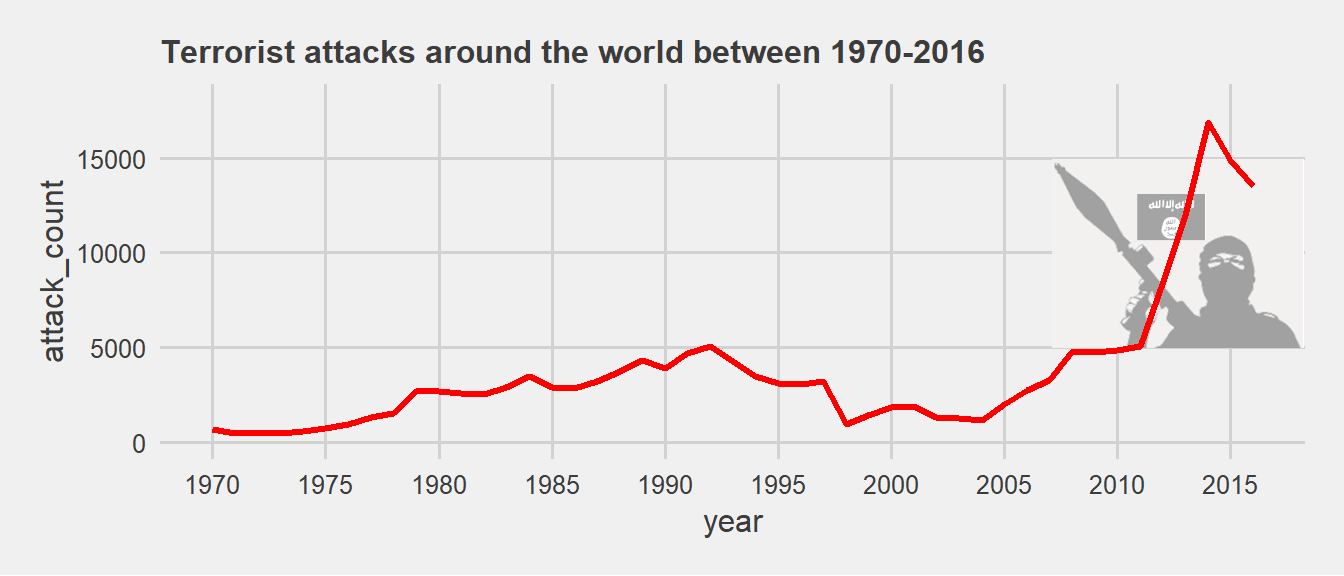
\includegraphics[width=1\linewidth]{thesis_files/figure-latex/unnamed-chunk-1-1} \caption{Terrorist attacks around the world between 1970-2016}\label{fig:unnamed-chunk-1}
\end{figure}
After September 2001 attacks, USA and other powerful nations have
carried out major operations to neutralize the power and spread of known
and most violent terrorist groups within the targeted region such as in
Afghanistan, Iraq and most recently in Syria. It's also worth mentioning
that the United Nations already have ongoing peacekeeping missions in
conflicted regions around the world for a long time. However number of
terror attacks continues to rise and in fact, it is almost on a peak in
the last 5 years. This leads to a question why terrorism is becoming
unstoppable despite the continued efforts. Understanding and
interpreting the attack characteristics of relevant groups in line with
their motivations to do so can reflect the bigger picture. An extensive
research by (Heger, 2010) supports this argument and suggests that a
group's political intentions are revealed when we examine who or what it
chooses to attack.

\hypertarget{research-design-and-data}{\section*{Research design and
data}\label{research-design-and-data}}
\addcontentsline{toc}{section}{Research design and data}

This research employs a mix of qualitative and quantitative research
methodology to achieve the set objective. In total, we evaluate cases of
over 170,000 terrorist attacks. We start with exploratory data analysis
to assess the impact on a global scale and then use a variety of data
mining techniques to determine the most active and violent terrorist
groups. This way, we ensure that the analysis reflects the situation in
present years. We use descriptive statistics to understand the
characteristics of each group over the period of time and locate the
major and minor epicenters (most vulnerable regions) based on threat
level. To examine whether or not chosen groups have a common link with
the number of fatalities, we perform statistical hypothesis test with
ANOVA and PostHoc test.

The research then makes use of a variety of machine learning algorithms
with supervised and unsupervised technique.
\begin{quote}
According to (Samuel, 1959), A well-known researcher in the field of
artificial intelligence who coined the term ``machine learning'',
defines machine learning as a ``field of study that gives computers the
ability to learn without being explicitly programmed''. It is a subset
of artificial intelligence which enables computers to learn from
experience in order to create inference over a possible outcome used
later to take a decision.
\end{quote}
With the Apriori algorithm, we discover interesting patterns through
association rules for individual groups. This way, we can pinpoint the
habits of specific groups. Next, we perform a time-series analysis to
examine seasonal patterns and correlations. To address the broad
question ``when and where'', we use four time-series forecasting models
namely Auto Arima, Neural Network, TBATS, and ETS to predict a future
number of attacks and fatalities. We evaluate and compare the
performance of each model on hold out set and use ensemble approach to
further improve the accuracy of predictions. As illustrated in
\protect\hyperlink{literature-review}{Literature review} section, most
research in time-series forecasting addresses the country and year level
predictions. We extend the previous research in this field with
seasonality component and make forecasts on a monthly frequency.
Similarly, in the classification modeling part, previous research lacks
the use of algorithms that are recently developed and that (practically)
out perform traditional algorithms such as logistic regression, random
forests etc. We extend the previous research in binary classification
context and make use of a cutting-edge LightGBM algorithm to predict the
class probability of an attack involving a suicide attempt. We
illustrate the importance of feature engineering and hyperparameter
optimization for modeling process and describe the reasons why standard
validation techniques such as cross-validation would be a bad choice for
this data. We propose an alternate strategy for validation and use AUC
metric as well as confusion matrix to evaluate model performance on
unseen data. From the trained model, we extract the most important
features and use explainer object to further investigate the
decision-making process behind our model. The scope of analysis can be
further extended with a shiny app which is also an integral part to make
this research handy and interactive.

\textbf{Data}

This research project uses historical data of terrorist attacks that
took place around the world between 1970 to 2016 from open-source
\href{https://www.start.umd.edu/gtd/about/}{Global Terrorism Database
(GTD)} as a main source of data. It is currently the most comprehensive
unclassified database on terrorist events in the world and contains
information on over 170,000 terrorist attacks. It contains information
on the date and location of the incident, the weapons used and the
nature of the target, the number of casualties and the group or
individual responsible if identifiable. The total number of variables is
more than 120 in this data. One of the main reason for choosing this
database is because 4,000,000 news articles and 25,000 news sources were
reviewed to prepare this data from 1998 to 2016 alone (National
Consortium for the Study of Terrorism and Responses to Terrorism
(START), 2016).

Main data is further enriched with country and year wise
socio-economical conditions, arms import/export details and migration
details from World Bank Open Data to get a multi-dimensional view for
some specific analysis. This additional data falls under the category of
early warning indicators (short term and long term) and potentially
linked to the likelihood of violent conflicts as suggested by the
researcher (Walton, 2011) and (Stockholm International Peace Research
Institute, 2017).

An important aspect of this research is a use of open-source data and
open-source software i.e.~R. The reason why media-based data source is
chosen as a primary source of data is that journalists are usually the
first to report and document such incidents and in this regard,
first-hand information plays a significant role in the quantitative
analysis. Since the source of data is from publicly available sources,
the term ``intelligence'' refers to the open-source intelligence (OSINT)
category. Intelligence categories are further explained in the next
chapter.

\section*{Policy and practice
implications}\label{policy-and-practice-implications}
\addcontentsline{toc}{section}{Policy and practice implications}

This research project is an endeavor to achieve actionable intelligence
using a machine learning approach and contributes positively to the
counterterrorism policy. The outcome of this research provides
descriptive findings of most lethal groups, corresponding pattern
discovery through Apriori algorithm and predictive analysis through
time-series forecasting and classification algorithm. Research findings
and insights will be helpful to policy makers or authorities to take
necessary steps in time to prevent future terrorist incidents.

\section*{Deliverables}\label{deliverables}
\addcontentsline{toc}{section}{Deliverables}
\begin{itemize}
\tightlist
\item
  a report in pdf version
\item
  a report in gitbook version
\item
  Shiny app
\item
  R scripts
\end{itemize}
To ensure that the research claims are (easily) reproducible, this
thesis uses rmarkdown and bookdown package which allows code execution
in line with a written report. \textbf{gitbook version} of this report
is highly recommended over pdf version because it allows interactivity
for some specific findings such as network graph in pattern discovery
chapter. In addition, a shiny app in R is developed to make the
practical aspects of this research handy, interactive and easily
accessible. This app also allows to further extending the scope of
analysis. All the scripts will be publicly accessible on my GitHub
profile\footnote{\url{https://github.com/pranavpandya84}} after
submission.

\hypertarget{essentials-counter}{\chapter{Essentials of
Counterterrorism}\label{essentials-counter}}

Terrorism research in broad context suggests that intelligence toward
counterterrorism support comes in many form. The primary objective of
this research is achieve actionable intelligence so it is important
identify the type of intelligence. In this chapter, we distinguish
between intelligence disciplines and then justify the reliability and
relevance of chosen data.

\section{Intelligence disciplines}\label{intelligence-disciplines}

An extensive research by (Tanner, 2014) suggests that establishing
methodologies for collecting intelligence is important for authorities/
policy makers to combat terrorism. The Intelligence Officer's Bookshelf
from CIA\footnote{\url{https://www.cia.gov/library/center-for-the-study-of-intelligence/csi-publications/csi-studies/studies/vol-60-no-1/pdfs/Peake-IO-Bookshelf-March-2016.pdf}}
recognizes Human Intelligence (HUMINT), Signals Intelligence (SIGINT),
Geospatial Intelligence (GEOINT), Measurement and Signature Intelligence
(MASINT) and Open Source Intelligence (OSINT) as five main disciplines
of intelligence collection (Lowenthal \& Clark, 2015).

\textbf{Human Intelligence (HUMINT)}

As the name suggests, HUMINT comes from human sources and remains
identical with espionage and clandestine activities. This is one of the
oldest intelligence techniques which use covert as well as overt
individuals to gather information. Example of such individuals can be
diplomats, special agents, field operatives or captured prisoners (The
Interagency OPSEC Support Staff, 1996). According to (CIA, 2013), human
intelligence plays vital role in developing and implementing U.S.
national security policy and foreign policy to protect U.S. interests.

\textbf{Signals Intelligence (SIGNIT)}

SIGNIT is derived from electronic transmissions such as by intercepting
communications between two channels/ parties. In the US, National
Security Agency (NSA) is primarily responsible for signals intelligence
(Groce, 2018). An example of SIGNIT is NSAs mass surveillance program
PRISM which is widely criticized due to dangers associated with it in
terms of misuse.
\begin{quote}
Edward Snowden, a former NSA contractor and source of the Guardian's
investigation on systematic data trawling by the US government, suggests
that, ``The reality is this: if an NSA, FBI, CIA, DIA {[}Defence
Intelligence Agency{]}, etc analyst has access to query raw SIGINT
{[}signals intelligence{]} databases, they can enter and get results for
anything they want. Phone number, email, user id, cell phone handset id
(IMEI), and so on -- it's all the same. The restrictions against this
are policy based, not technically based, and can change at any time.''
(Siddique, 2013)
\end{quote}
\textbf{Geospatial Intelligence (GEOINT)}

GEOINT makes use of geo-spatial analysis and visual representation of
activities on the earth to examine suspicious activities. This is
usually carried out by observation flights, UAVs, drones and satellites
(Brennan, 2016).

\textbf{Measurement and Signature Intelligence (MASINT)}

MASINT is comparatively less known methodology however it's becoming
extremely important when concerns about WMDs (Weapons of Mass
Destruction) are increasing. This approach peforms analysis of data from
specific sensors for the purpose of identifying any distinctive features
associated with the source emitter or sender. This analysis serves as
scientific and technical intelligence information. An example of MASINT
is FBI's extensive forensic work that helps detecting traces of nuclear
materials, chemical and biological weapons (Groce, 2018).

\textbf{Open Source Intelligence (OSINT)}

OSINT is relatively new approach that focuses on publicly available
information and sources such as newspaper articles, academic records and
open-source data made available to public from government or
researchers. The key advantage of open source intelligence is
accessibility and makes it possible for individual researchers to
contribute toward counter terrorism support as a part of community. It
is important to note that reliability of data source can be complicated
and thus requires review in order to be a use to policy makers (Groce,
2018; Tanner, 2014).

Focus and scope of work for this research is limited to Open Source
Intelligence only.

\section{OSINT and data relevance}\label{osint-and-data-relevance}

Despite the huge (and technically limitless) potential for counter
terrorism support, the reason as to why open source intelligence is
often reviewed and analysed before it can be used by policy makers is
because of complications related to authenticity of data source and
methodology used to compile data for hypothesis testing by a researcher.
In simple words what it means is, it is extremely important for policy
makers to ensure that there is no selection bias or cherry-picking from
a researcher to claim the success of particular theory or results
(Brennan, 2016). A research paper from (Geddes, 1990/ed) namely
``\emph{How the Cases You Choose Affect the Answers You Get: Selection
Bias in Comparative Politics}'' explains the danger of biased
conclusions when the cases that have achieved the outcome of interest
are studied. This clearly forms the need for reproducible research and
allows authorities to set the standard/ mechanism to safe guard against
selection bias. This is particularly important in terrorism research.
This critical issue can be taken care by codes/ scripts shared through
git repositories. Nowadays, making use of tools such as rmarkdown and
bookdown to deliver reproducible research (Bauer, 2018; Xie, 2016) makes
it even easier to identify selection bias.

\subsection{Open-source databases on
terrorism}\label{open-source-databases-on-terrorism}

In the context of terrorism research, there are many databases available
for academic research. Such databases extracts and compile information
from variety of sources (mainly open-source/ publicly available sources
such as news articles) on regular interval and makes it easy to use for
research. Some of the well-known databases that are open-source and
widely used in academic research for counter terrorism support are as
below:

\textbf{1. Global Terrorism Database (GTD)}\footnote{\url{http://www.start.umd.edu/gtd/about/}}
\begin{itemize}
\tightlist
\item
  Currently the most comprehensive unclassified database on terrorist
  events in the world
\item
  maintained by researchers at the National Consortium for the Study of
  Terrorism and Responses to Terrorism (START), headquartered at the
  University of Maryland in the USA
\end{itemize}
\textbf{2. Armed Conflict Location and Event Data Project
(ACLED)}\footnote{\url{https://www.acleddata.com/data/}}
\begin{itemize}
\tightlist
\item
  provides real-time data on all reported political violence and protest
  events however limited to developing countries i.e.~Africa, South
  Asia, South East Asia and the Middle East
\end{itemize}
\textbf{3. UCDP/PRIO Armed Conflict Database}\footnote{\url{https://www.prio.org/Data/Armed-Conflict/UCDP-PRIO/}}
\begin{itemize}
\tightlist
\item
  a joint project between the UCDP and PRIO that records armed conflicts
  from 1946--2016
\item
  maintained by Uppsala University in Sweden
\end{itemize}
\textbf{4. SIPRI Databases}\footnote{\url{https://www.sipri.org/databases}}
\begin{itemize}
\tightlist
\item
  provides databases on military expenditures, arms transfers, arms
  embargoes and peacekeeping operations
\item
  maintained by Stockholm International Peace Research Institute
\end{itemize}
In order to address the research objective, I find the Global Terrorism
Database most relevant and it is the main source of data for this
research. As mentioned in
\protect\hyperlink{research-design-and-data}{Research design and data}
section, main data is further enriched with world development indicators
for each countries by year from World Bank Open Data.\footnote{\url{https://data.worldbank.org/}}

\section{What's important in terrorism
research?}\label{whats-important-in-terrorism-research}

Aim of any research can be seen as an effort toward creating new
knowledge, insights or a perspective. In this regard, careful selection
of data source and corresponding statistical analysis based on research
objective is extremely important. Equally important aspect is to share
the data and codes so that research claims or findings can be
reproduced. This also forms the basis for the trustworthiness and
usefulness of the research outcome.

\subsection{Primary vs secondary
sources}\label{primary-vs-secondary-sources}

The term ``sources'' refers to data or a material used in research and
has two distinct categories. The primary sources provide first hand
information about an incident. Secondary sources are normally based on
primary sources and provide interpretive information about an incident
(Indiana University Libraries, 2007). For example, propaganda video/
speech released by ISIL or any other terrorist group are a primary
source whereas newspaper article that publishes journalist's
interpretation of that speech becomes secondary source. Researcher
(Schuurman, 2018) suggests that, in such scenarios, the difference is
not always distinguishable because it depends on the type of question
being asked. Contrary to popular belief, newspaper or media articles are
considered a secondary source of information about terrorism and
terrorists. However news or media articles can be considered as primary
source of information when the research focuses on how media reports on
terrorism (Schuurman, 2018). In our case, the main source of data is
through news and media articles about reported terrorist incidents and
fits the category of primary source of data based on research objective.

\subsection{Use of statistical
analysis}\label{use-of-statistical-analysis}

In most areas of scientific analysis, statistics is often considered as
an important and accepted way to ensure that claims made by researchers
meet defined quality standards (Ranstorp, 2006). To be specific,
descriptive statistics helps describing variables within data and often
used to perform initial data analysis in most research. On the other
hand, inferential statistics helps drawing conclusions/ decisions based
on observed patterns (Patel, 2009).

A prominent researcher (Andrew Silke, 2004), in his book
``\emph{Research on Terrorism: Trends, Achievements and Failures}'',
explains why inferential statistics is significantly important in
terrorism research context. The author suggests that inferential
statistics is useful to introduce element of control into research. In
an experimental research, control is usually obtained by random
assignment of research subjects to experimental and control groups
however it's difficult achieve in real world research. As a result, lack
of control element raises doubt on any relations between variables which
the research claims to find. As a solution, inferential statistics can
help to introduce recognized control element within research and so that
less doubt and more confidence can be achieved over the veracity of
research outcome.

\hypertarget{literature-review}{\chapter{Literature
Review}\label{literature-review}}

I use a structured approach to narrow down recent and relevant
literature. In this chapter, we take a glimpse of prior research in this
field and review the relevant literature in line with factors identified
in \protect\hyperlink{essentials-counter}{Essentials of
Counterterrorism} chapter. In the last part, we examine the literature
gap and relevance with our research topic.

\section{Overview of prior research}\label{overview-of-prior-research}

Scientific research in the field of terrorism is heavily impacted by
research continuance issue. According to (Gordon, 2007), there is indeed
a growing amount of literature in terrorism field but the majority of
contributors are one-timers who visit and study this field, contribute
few articles, and then move to another field. Researcher (Schuurman,
2018) points out another aspect and suggests that terrorism research has
been criticized for a long time for being unable to overcome
methodological issues such as high dependency on secondary sources,
corresponding literature review methods and relatively insufficient
statistical analyses. This argument is further supported a number of
prominent researchers in this field. Compared to other similar fields
such as criminology, terrorism research suffers a lot due to
complications in data availability, reliability and corresponding
analysis to make the research useful to policymakers (Brennan, 2016).

\subsection{Harsh realities}\label{harsh-realities}

One of the harsh realities in terrorism research is that the use of
statistical analysis is fairly uncommon. In late 80s, (Jongman, 1988) in
his book ``\emph{Political Terrorism: A New Guide To Actors, Authors,
Concepts, Data Bases, Theories, And Literature}'' identified serious
concerns in terrorism research related to methodologies used by the
researcher to prepare data and corresponding level of analysis. (A.
Silke, 2001) reviewed the articles in terrorism research between 1995
and 2000 and suggests that key issues raised by (Jongman, 1988) remains
unchanged in that period as well. Their research findings indicate that
only 3\% of research papers involved the use of inferential analysis in
the major terrorism journals. Similar research was carried out by (Lum,
Kennedy, \& Sherley, 2006) on quality of research articles in terrorism
research and their finding suggests that much has been written on
terrorism between 1971 to 2003 and around 14,006 articles were published
however the research that can help/support counterterrorism strategy was
extremely low. This study also suggests that only 3\% of the articles
were based on some form of empirical analysis, 1\% of articles were
identified as case studies and rest of the articles (96\%) were just
thought pieces.

Very recently, researcher (Schuurman, 2018) also conducted an extensive
research to review all the articles (3442) published from 2007 to 2016
in nine academic journals on terrorism and provides an insight on
whether or not the trend (as mentioned) in terrorism research continues.
Their research outcome suggests an upward trend in on the use of
statistical analysis however major proportion is related to descriptive
analysis only. They selected 2552 articles for analysis and their
findings suggest that:
\begin{itemize}
\tightlist
\item
  only \textbf{1.3\%} articles made use of inferential statistics
\item
  5.8\% articles used mix of descriptive and inferential statistics
\item
  14.7\% articles used descriptive statistics and
\item
  78.1\% articles did not use any kind of statistical analysis
\end{itemize}
\begin{figure}
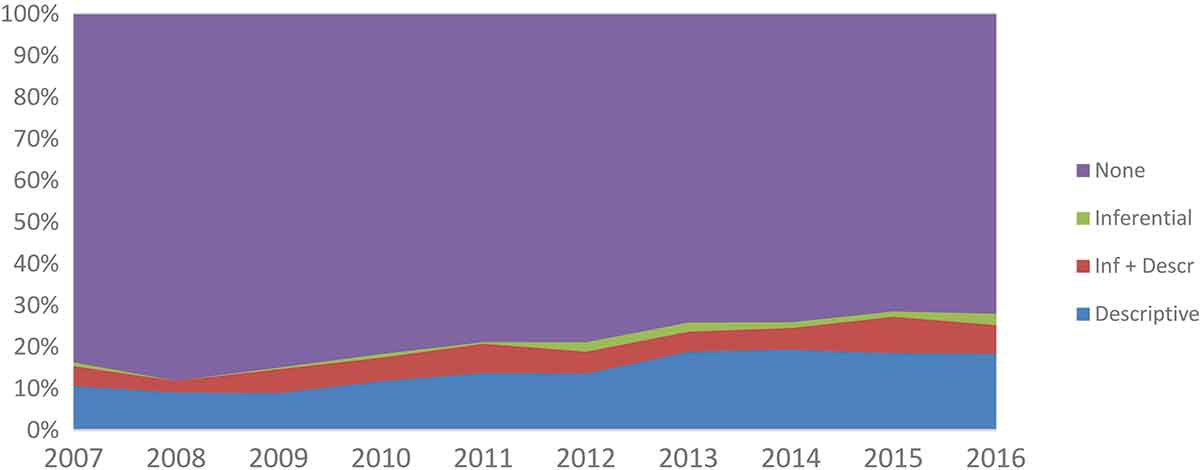
\includegraphics[width=1\linewidth]{figure/research_stats} \caption{Use of statistics in terrorism research from 2007 to 2016}\label{fig:stats1}
\end{figure}
(Schuurman, 2018)

\subsection{Review of relevant
literature}\label{review-of-relevant-literature}

In this section, we take a look at previous research that is intended
toward counterterrorism support while making sure that the chosen
research article/ literature contains at least some form of statistical
modeling.

Simple linear regression was one of the approaches for prediction models
in early days but soon it was realized that such models are weak in
capturing complex interactions. The emergence of machine learning
algorithms and advancement in deep learning made it possible to develop
fairly complex models however country-level analysis with resolution at
year level contributes majority of research work in conflict prediction
(Cederman \& Weidmann, 2017).

(Beck, King, \& Zeng, 2000) carried out a research to stress the
important of the causes of conflict. Researchers claim that empirical
findings in the literature of global conflict are often unsatisfying,
and accurate forecasts are unrealistic despite availability immense data
collections, notable journals, and complex analyses. Their approach uses
a version of a neural network model and argues that their forecasts are
significantly better than previous effort.

In a study to investigate the factors that explain when terrorist groups
are most or least likely to target civilians, researcher (Heger, 2010)
examines why terrorist groups need community support and introduces new
data on terrorist groups. The research then uses logit analysis to test
the relationship between independent variables and civilian attacks
between 1960-2000.

In a unique and interesting approach, a researcher from ETH Zürich
(Chadefaux, 2014) examines a comprehensive dataset of historical
newspaper articles and introduces weekly risk index. This new variable
is then applied to a dataset of all wars reported since 1990. The
outcome of this study suggests that the number of conflict-related news
items increases dramatically prior to the onset of conflict. Researcher
claims that the onset of a war data within the next few months could be
predicted with up to 85\% confidence using only information available at
the time. Another researcher (Cederman \& Weidmann, 2017) supports the
hypothesis and suggests that news reports are capable to capture
political tension at a much higher temporal resolution and so that such
variables have much stronger predictive power on war onset compared to
traditional structural variables.

One of the notable (and publicly known) researches in terrorism
predicted the military coup in Thailand 1 month before its actual
occurrence on 7 May 2014. In a report commissioned by the CIA-funded
Political Instability Task Force, researchers (Ward Lab, 2014)
forecasted irregular regime changes for coups, successful protest
campaigns, and armed rebellions, for 168 countries around the world for
the 6-month period from April to September 2014. Researchers claim that
Thailand was number 4 on their forecast list. They used an ensemble
model that combines seven different split-population duration models.

Researchers (Fujita, Shinomoto, \& Rocha, 2016) use high temporal
resolution data across multiple cities in Syria and time-series
forecasting method to predict future event of deaths in Syrian armed
conflict. Their approach uses day level data on death tolls from
Violations Documentation Centre (VDC) in Syria. Using Auto-regression
(AR) and Vector Auto-regression (VAR) models, their study identifies
strong positive auto-correlations in Syrian cities and non-trivial
cross-correlations across some of them. Researchers suggest that strong
positive auto-correlations possibly reflects a sequence of attacks
within short periods triggered by a single attack, as well as
significant cross-correlation in some of the Syrian cities imply that
deaths in one city were accompanied by deaths at another city.

Within a pattern recognition context, researchers (Klausen, Marks, \&
Zaman, 2016) from MIT Sloan developed a behavioural model to predict
which Twitter users are likely belonged to the Islamic state group.
Using data of approximately 5,000 Twitter users who were linked with
Islamic state group members, they created a dataset of 1.3 million users
by associating friends and followers of target users. At the same time,
they monitored Twitter over few months to identify which profiles are
getting suspended. Researchers claim that they were able to train a
machine learning model that matched suspended accounts with the
specifics of the profile and creating a framework to identify likely
members of ISIL.

A similar research from (Ceron, Curini, \& Iacus, 2018) examines over 25
million tweets in Arabic language when Islamic State was at its peak
strength (between Jan 2014 to Jan 2015) and was expanding regions under
its control. Researchers assessed the share of support from the online
Arab community toward ISIS and investigated time time-granularity of
tweets while linking the tweet opinions with daily events and
geolocation of tweets. The outcome of their research finds a
relationship between foreign fighters joining ISIS and online opinions
across the regions.

One of the researches evaluates the targeting patterns and preferences
of 480 terrorist groups that were operational between 1980 and 2011 in
order to find the impact of longetivity of terrorist groups based on
their lethality. Based on group-specific case studies on the Afghan and
Pakistani Taliban and Harmony Database from Combat Terrorism Centre,
researcher (Nawaz, 2017) uses Bivariate Probit Model to assess the
endogenous relationship and finds significant correlationship between
negative group reputation and group mortality. The researcher also uses
Cox Proportional Hazard Model to estimate longetivity of group.

(Colaresi \& Mahmood, 2017) carried out a research to identify and avoid
the problem of overfitting sample data. Researchers used the models of
civil war onset data and came up with a tool (R package: ModelCriticism)
to illustrate how machine learning based research design can improve out
of fold forecasting performance. Their study recommends making use of
validation split along with train and test split to benefit from
iterative model criticism.

Researchers (Muchlinski, Siroky, He, \& Kocher, 2016/ed) use The Civil
War Data (1945-2000) and compared the performance of Random Forests
model with three different versions of logistic regression. The outcome
of their study suggests that random forest model provides significantly
more accurate predictions on the occurrences of rare events in out of
sample data compared to logistic regression models on a chosen dataset.
However in an experimental research to reproduce this claims,
(Neunhoeffer \& Sternberg, 2018) ran re-analysis and finds problematic
usage of cross-validation strategy. They contest the claim and suggest
that there is no evidence of significant predictive performance of
random forest as claimed by the original authors.

\subsection{GTD and machine learning in previous
research}\label{gtd-and-machine-learning-in-previous-research}

Addressing the issue of rare events, researchers (Clauset \& Woodard,
2013) came up with statistical modelling approach to estimate future
probability of large scale terrorist attack. Using the data from GTD and
RAND-MIPT database between 1968-2007, and three different models
i.e.~power law, exponential distributions and log normal, researchers
estimate the likelihood of observing 9/11 sized attack between 11-35\%.
Using the same procedure, researchers then make a data-driven
statistical forecast of at least one similar event over the next decade.

In a study to identify determinants of variation in country compliance
with financial counterterrorism, researcher (Lula, 2014) uses dataset on
financial counterterrorism for the period 2004-2011 along with Global
Terrorism Database. Researcher employs both quantitative and qualitative
analysis in their approach and uses regression analysis (ordered logit
model) to estimate the statistical significance of independent variables
on target variable i.e.~compliance rates. The outcome of this study
suggests that intensity and magnitude of terror threat, rate of
international terror attacks, rate of suicide (terror) attacks, and
military capability variable does not have a statistically significant
effect on country compliance with financial counterterrorism. Based on
research findings, the author suggests that many of the assumptions made
in the previous study in financial counterterrorism are incorrect.

A research from (Brennan, 2016) uses machine learning based approach to
investigate terrorist incidents by country. This study makes use of
regression techniques, Hidden Markov model, twitter outbreak detection
algorithm, SURUS algorithm, as well as medical syndromic surveillance
algorithms i.e EARSC based method and Farrington's method to detect
change in behaviour (in terms of terrorist incident or fatalities). The
outcome of their study suggests that time-series aberration detection
methods were highly interpretable and generalizable compared to
traditional methods (regression and HMM) for analysing time series data.

Researcher (Block, 2016) carried out a study to identify characteristics
of terrorist events specific to aircrafts and airports and came up with
situation crime prevention framework to minimize such attacks. In
particular, the researcher uses GTD data (2002-2014) specific to attacks
involving airports/ aircraft that contains terrorist events related to
44 nations. In this study, Logistic Regression model is used to evaluate
variables that are significantly associated with such attacks. Their
research findings suggest that the likelihood of attacks against
airports is mostly related to domestic terrorist groups and, explosives
and suicide attacks as a type of attack. In contrast, attacks against
aircraft are more associated with international terrorists groups.

In an effort to improve accuracy of classification algorithms,
researchers (Mo, Meng, Li, \& Zhao, 2017) uses GTD data and employs
feature selection methods such as Minimal-redundancy maximal-relevancy
(mRMR) and Maximal relevance (Max-Relevance). In this study, researchers
use Support Vector Machine, Naive Bayes, and Logistic Regression
algorithms and evaluate the performance of each model through
classification precision and computational time. Their research finding
suggests that feature selection methods improve the accuracy of the
model and comparatively, Logistic Regression model with seven optimal
feature subset achieves a classification precision of 78.41\%.

A research from (Ding, Ge, Jiang, Fu, \& Hao, 07AD--2017) also uses
classification technique to evaluate risk of terrorist incident at
global level using GTD and several other datasets. In particular, data
comprising terror incidents between 1970 to 2015 was used to train and
evaluate neural network (NNET), support vector machine (SVM), and random
forest (RF) models. For performance evaluation, researchers used
three-quarters of the randomly sampled data as a training set, and the
remaining as a test set. The outcome of their study predicted the places
where terror events might occur in 2015, with a success rate of 96.6\%.

In a similar research within classification context and addressing the
issue of class unbalance in order to predict rare events
i.e.~responsible group behind terror attack, researchers (Gundabathula
\& Vaidhehi, 2018) employ various classification algorithms in line with
sampling technique to improve the model accuracy. In particular, this
study was narrowed down to terrorist incidents in India and data used
from GTD was between 1970-2015. Researchers used J48, IBK, Naive Bayes
algorithms and an ensemble approach for the classification task. Finding
from their study indicates the importance of using sampling technique
which improves the accuracy of base models and suggests that an ensemble
approach improves the overall accuracy of base models.

\section{Literature gap and
relevance}\label{literature-gap-and-relevance}

Review of the recent and relevant literature suggests that use of
historical data from open source databases, and statistical modeling
using time-series forecasting algorithms are commonly used approach to
address the research questions related to ``when and where''. A trend
can be seen in the research study with a variety of new approaches such
as feature selection, sampling technique, validation split etc to
achieve better accuracy in classification algorithms. This is one of the
most relevant aspects of this research project.

While some approach argues that prediction is a contentious issue and
focuses on finding causal variables while neglecting model fit, there is
an upward trend in an approach that uses diverse models, and out of fold
method which also allows evaluating and comparing model performance.
Similarly, a single model philosophy based on Occam's razor principle is
visible in some of the research however ensemble philosophy to make use
of weak but diverse models to improve the overall accuracy is gaining
popularity amongst research nowadays.

It is also observed that use of gradient boosting machines is not
popular in scientific research despite the availability and practical
use cases of highly efficient and open-source algorithms such as XGBoost
and LightGBM which are widely used in machine learning competitions such
as Kaggle. In contrast, traditional algorithms such as Random Forest,
Logistic Regression, Naive Bayes, J48 etc. are often used in majority of
research.

One important observation from the literature review is that code
sharing is quite uncommon. Replication crisis is a major issue in
scientific research. Despite the availability of a number of open source
tools for reproducible research such as Jupyter notebook, rmarkdown or
code repositories such as github, the majority of research papers lacks
code sharing aspect.

\hypertarget{impact-analysis}{\chapter{Impact
Analysis}\label{impact-analysis}}

This part of the research uses descriptive statistics to explore and
understand terrorist events from various perspectives. This is essential
to examine characteristics of attacks and responsible groups over the
period of time. Findings and insights from this analysis are eventually
helpful to select appropriate data for the statistical modeling part.

\section{Data preparation}\label{data-preparation}

The primary data file \texttt{globalterrorismdb\_0617dist.xlsx} used in
this research contains over 170,000 terrorist attacks between 1970-2016
(excluding the year 1993). This file can be downloaded by filling up a
form on START Consortium's website.\footnote{Accessing GTD data:
  \url{https://www.start.umd.edu/gtd/contact/}} This file contains a
total of 135 variables categorized by incident ID and date, incident
information, attack information, weapon information, target/victim
information, perpetrator information, casualties and consequences, and
additional information. Out of 135 variables, I have selected a total of
38 variables from each category that are relevant to the research
objective. During the data cleaning process, I have made following
changes (corrective steps) to original data to make it ready for
analysis:
\begin{itemize}
\tightlist
\item
  renaming of some variables (such as \texttt{gname} to
  \texttt{group\_name}, \texttt{INT\_LOG} to
  \texttt{intl\_logistical\_attack}) to keep the analysis and codes
  interpretable to a wider audience.
\item
  replacing 2.7\% NAs in latitude and longitude with country level or
  closest matching geocodes. Note that most NAs refers to either
  disputed territories such as Kosovo or countries that no longer exist
  such as Czechoslovakia.
\item
  5\% NAs in \texttt{nkill} (number of people killed) and 9\% NAs in
  \texttt{nwound} (number of people wounded) variable replaced with 0.
  GTD reference manual suggests that ``Where there is evidence of
  fatalities, but a figure is not reported or it is too vague to be of
  use, this field remains blank.''
\item
  NAs in regional variables i.e \texttt{city} and \texttt{provstate}
  replaced with ``unknown''
\end{itemize}
GTD data is further enriched with country and year wise indicators from
World Bank Open Data to get a multi-dimensional view and for modeling
part. This data is also open-source and can be accessed through R
library \texttt{WDI}.\footnote{Searching and extracting data from the
  World Bank's World Development Indicators. :
  \url{https://cran.r-project.org/web/packages/WDI/WDI.pdf}}

List of all the variable with a short description as well as the script
to implement the aforementioned steps and to prepare clean dataset can
be viewed in \protect\hyperlink{appendix-i}{Appendix I}. Detailed
information and explanation about each variable can be found GTD
codebook\footnote{\url{https://www.start.umd.edu/gtd/downloads/Codebook.pdf}}.

\section{Global overview}\label{global-overview}
\begin{Shaded}
\begin{Highlighting}[]
\NormalTok{tmp <-}\StringTok{ }\NormalTok{df }\OperatorTok\StringTok{ }\KeywordTok{group_by}\NormalTok{(region, year) }\OperatorTok\StringTok{ }\KeywordTok{summarize}\NormalTok{(}\DataTypeTok{attack_count =} \KeywordTok{n}\NormalTok{())}
\end{Highlighting}
\end{Shaded}
A quick look at region level number attacks suggests that situation is
becoming worst in the Middle East \& North Africa followed by South
Asia, Sub-Saharan Africa and Southeast Asia where exponential growth in
a number of attacks can be observed specifically from years 2010 to
2016. Note that the Y-axis is set free to have closer look at trends.
\begin{figure}
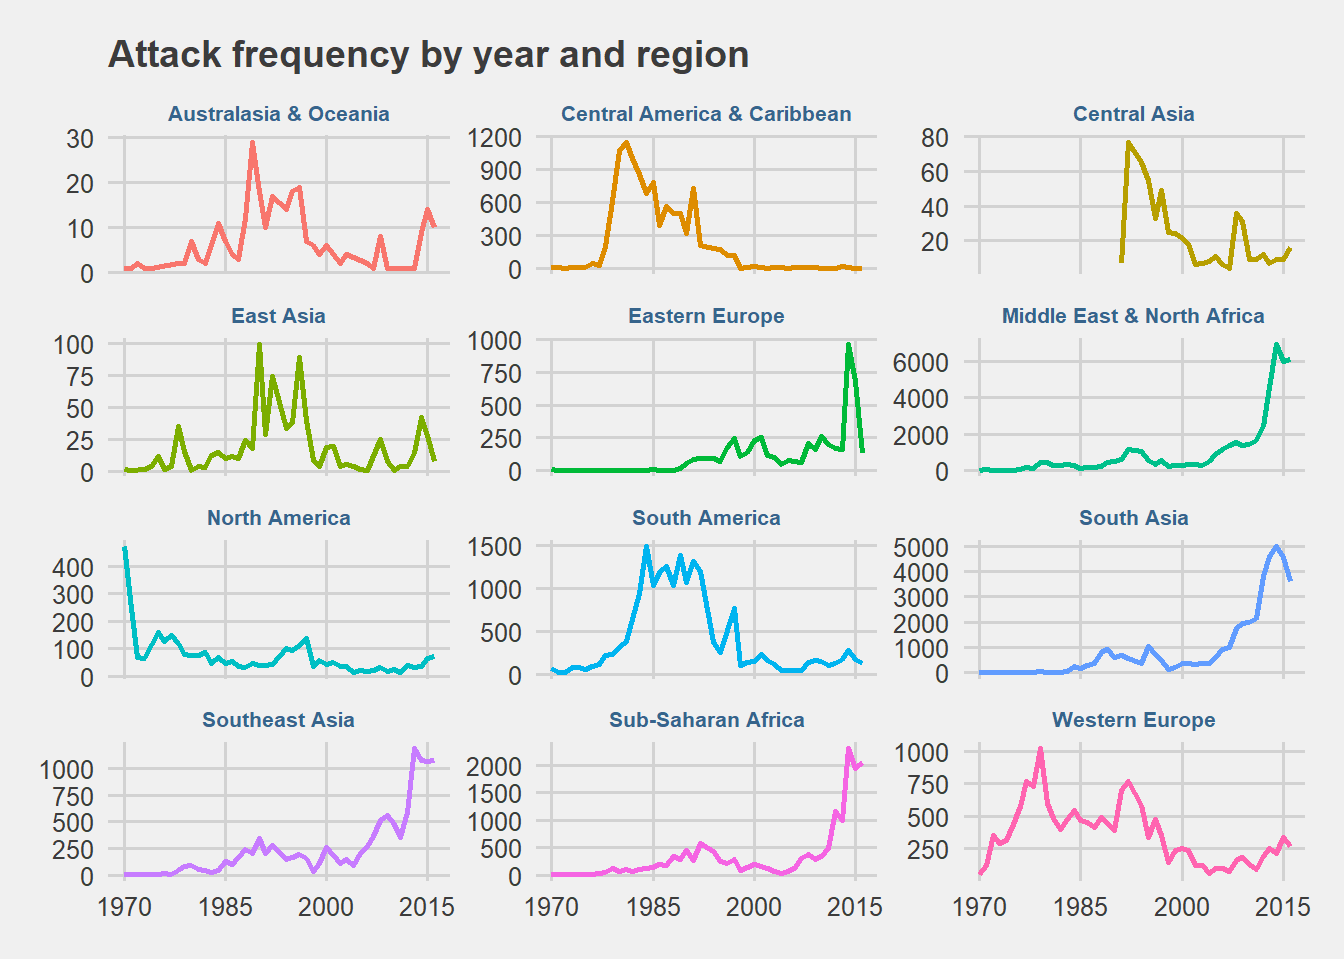
\includegraphics[width=1\linewidth]{thesis_files/figure-latex/unnamed-chunk-3-1} \caption{Attack frequency by year and region}\label{fig:unnamed-chunk-3}
\end{figure}
An interesting observation is in Eastern Europe region where a sudden
increase in a number of attacks can be observed during 2014-2015 and
then a sudden decrease in 2016. Within the most impacted regions, the
nearly similar trend of gradual increase in a number of attacks after
2010 and peak during 2014-2015 is visible. It's worth mentioning that in
June 2014, Islamic State announced the establishment of ``Caliphate''
while declaring Abu Bakr al-Baghdadi as ``leader of Muslims everywhere''
and urging other groups to pledge allegiance (Al Jazeera, 2014). Islamic
State was at its peak strength during Jan 2014 to Jan 2015 (Ceron et
al., 2018).

To understand the attack characteristics, let's take a look at Frequency
of attack type and type of weapon used by terrorist groups.
\begin{Shaded}
\begin{Highlighting}[]
\NormalTok{tmp <-}\StringTok{ }\NormalTok{df }\OperatorTok\StringTok{ }\KeywordTok{group_by}\NormalTok{(attack_type, year) }\OperatorTok\StringTok{ }\KeywordTok{summarise}\NormalTok{(}\DataTypeTok{total_attacks =} \KeywordTok{n}\NormalTok{()) }
\end{Highlighting}
\end{Shaded}
\begin{figure}
\includegraphics[width=1\linewidth]{figure/heatmap_attack} \caption{Trend in type of attack in all incidents globally}\label{fig:unnamed-chunk-5}
\end{figure}
The heat signatures indicate Bombing/Explosive as one of the frequently
used techniques by terrorist groups. Although the pattern in this tactic
is visible throughout all the year, while rising during the late 80s and
early 90s however it has now increased to nearly 7 times since 2006. A
similar pattern (with lower magnitude) can be observed in Armed Assault
followed by Hostage Taking and Assassination technique.
\begin{Shaded}
\begin{Highlighting}[]
\NormalTok{tmp <-}\StringTok{ }\NormalTok{df }\OperatorTok\StringTok{ }\KeywordTok{group_by}\NormalTok{(weapon_type, year) }\OperatorTok\StringTok{ }\KeywordTok{summarise}\NormalTok{(}\DataTypeTok{total_attacks =} \KeywordTok{n}\NormalTok{())}
\end{Highlighting}
\end{Shaded}
\begin{figure}
\includegraphics[width=1\linewidth]{figure/heatmap_weapon} \caption{Trend in type of weapon used in all incidents globally}\label{fig:unnamed-chunk-7}
\end{figure}
Upon examining the trends in the type of weapon used in all terrorist
incidents globally, it is visible that use of Explosives/Bomb/Dynamites
and Firearms is extremely high since 2011 and compared to other weapon
types. Use of vehicles as weapon type was relatively low until 2013,
however, it was on peak in 2015 with total 34 number of attacks.

Observing trends in target type over the period of time is also a useful
way to understand characteristics and ideology among terrorist
incidents. As shown in the plot below, the heat signature indicates the
top five most frequently attacked target types as Private Citizens \&
Property followed by Military, Police, Government, and Business.
\begin{Shaded}
\begin{Highlighting}[]
\NormalTok{tmp <-}\StringTok{ }\NormalTok{df }\OperatorTok\StringTok{ }\KeywordTok{group_by}\NormalTok{(target_type, year) }\OperatorTok\StringTok{ }\KeywordTok{summarise}\NormalTok{(}\DataTypeTok{total_attacks =} \KeywordTok{n}\NormalTok{()) }
\end{Highlighting}
\end{Shaded}
\begin{figure}
\includegraphics[width=1\linewidth]{figure/heatmap_target} \caption{Trend in intended targets in all incidents globally}\label{fig:unnamed-chunk-9}
\end{figure}
According to GTD codebook, Private Citizens \& Property category
includes attack on individuals, public in general or attacks in highly
populated areas such as markets, commercial streets, busy intersections
and pedestrian malls. In a study to investigate when terrorist groups
are most or least likely to attack civilians, researcher (Heger, 2010)
find a relationship with group's political motivation and suggests that
terror groups pursuing a nationalist agenda are more likely to attack
civilians. A relatively lower magnitude trend but with gradual increase
in recent years is also visible on Religious Figures/Institution and
Terrorist/ Non-state Militia category. The inclusion criteria for
Terrorist/ Non-state Militia category refers to terrorists or members of
terrorist groups (that are identified in GTD) and broadly defined as
informants for terrorist groups excluding former or surrendered
terrorists.

\section{The top 10 most active and violent
groups}\label{the-top-10-most-active-and-violent-groups}

Findings from exploratory data analysis at region level indicate that
the number of attacks have increased significantly from the year 2010
and nearly at the same pace in the Middle East \& North Africa, South
Asia, Sub-Saharan Africa and Southeast Asia region. Trends in attack
type, weapon type and target type over the same period of time (from
2010) suggests that bombings and explosions as a choice of attack type
is growing exponentially while the use of explosives \& firearms and
attacks on civilians is at alarming high level.

This part of the research identifies and examines the top ten most
violent and active terrorist groups based on a number of fatalities and
number of people injured. GTD codebook suggests that when an attack is a
part of multiple attacks, sources sometimes provide a cumulative
fatality total for all of the incidents rather than fatality figures for
each incident.

In order to determine top ten most active and violent groups based on
fatalities and injured while preserving statistical accuracy, first I
filter the dataset for the events that took place from 2010 onward and
remove the incidents where group name is not known. The new variable
\texttt{impact} is the sum of fatalities and the number of people
injured. Wherever an attack is observed as a part of multiple attacks,
and reported figures are different, I use the figure which is maximum
among all the reported figures while ensuring that reported incidents
are distinct and grouped by month, year, region and name of the group as
shown in the code below:
\begin{Shaded}
\begin{Highlighting}[]
\NormalTok{by_groups <-}\StringTok{ }\NormalTok{df }\OperatorTok\StringTok{ }
\StringTok{  }\KeywordTok{filter}\NormalTok{(group_name }\OperatorTok{!=}\StringTok{ "Unknown"} \OperatorTok{&}\StringTok{ }\NormalTok{year }\OperatorTok{>=}\StringTok{ }\DecValTok{2010}\NormalTok{) }\OperatorTok\StringTok{ }
\StringTok{  }\KeywordTok{replace_na}\NormalTok{(}\KeywordTok{list}\NormalTok{(}\DataTypeTok{nkill =} \DecValTok{0}\NormalTok{, }\DataTypeTok{nwound =} \DecValTok{0}\NormalTok{)) }\OperatorTok\StringTok{ }
\StringTok{  }\KeywordTok{select}\NormalTok{(group_name, region, year, month, nkill, nwound, }
\NormalTok{         part_of_multiple_attacks) }\OperatorTok\StringTok{ }
\StringTok{  }\KeywordTok{group_by}\NormalTok{(group_name, region, year, month) }\OperatorTok\StringTok{ }
\StringTok{  }\KeywordTok{filter}\NormalTok{(}\KeywordTok{if_else}\NormalTok{(part_of_multiple_attacks }\OperatorTok{==}\StringTok{ }\DecValTok{1}\NormalTok{, }
\NormalTok{                 nkill }\OperatorTok{==}\StringTok{ }\KeywordTok{max}\NormalTok{(nkill) }\OperatorTok{&}\StringTok{ }\NormalTok{nwound }\OperatorTok{==}\StringTok{ }\KeywordTok{max}\NormalTok{(nwound), }
\NormalTok{                 nkill }\OperatorTok{==}\StringTok{ }\NormalTok{nkill }\OperatorTok{&}\StringTok{ }\NormalTok{nwound }\OperatorTok{==}\StringTok{ }\NormalTok{nwound)) }\OperatorTok
\StringTok{  }\KeywordTok{distinct}\NormalTok{(group_name, region, year, month, nkill, nwound, }
\NormalTok{           part_of_multiple_attacks) }\OperatorTok
\StringTok{  }\KeywordTok{mutate}\NormalTok{(}\DataTypeTok{impact =}\NormalTok{ nkill }\OperatorTok{+}\StringTok{ }\NormalTok{nwound) }\OperatorTok
\StringTok{  }\KeywordTok{group_by}\NormalTok{(group_name) }\OperatorTok
\StringTok{  }\KeywordTok{summarise}\NormalTok{(}\DataTypeTok{total =} \KeywordTok{sum}\NormalTok{(impact)) }\OperatorTok\StringTok{ }
\StringTok{  }\KeywordTok{arrange}\NormalTok{(}\KeywordTok{desc}\NormalTok{(total)) }\OperatorTok\StringTok{ }
\StringTok{  }\KeywordTok{head}\NormalTok{(}\DecValTok{10}\NormalTok{)}

\CommentTok{# create a vector of top 10 groups for further analysis}
\NormalTok{top10_groups <-}\StringTok{ }\KeywordTok{as.vector}\NormalTok{(by_groups}\OperatorTok{$}\NormalTok{group_name)}
\end{Highlighting}
\end{Shaded}
\begin{figure}
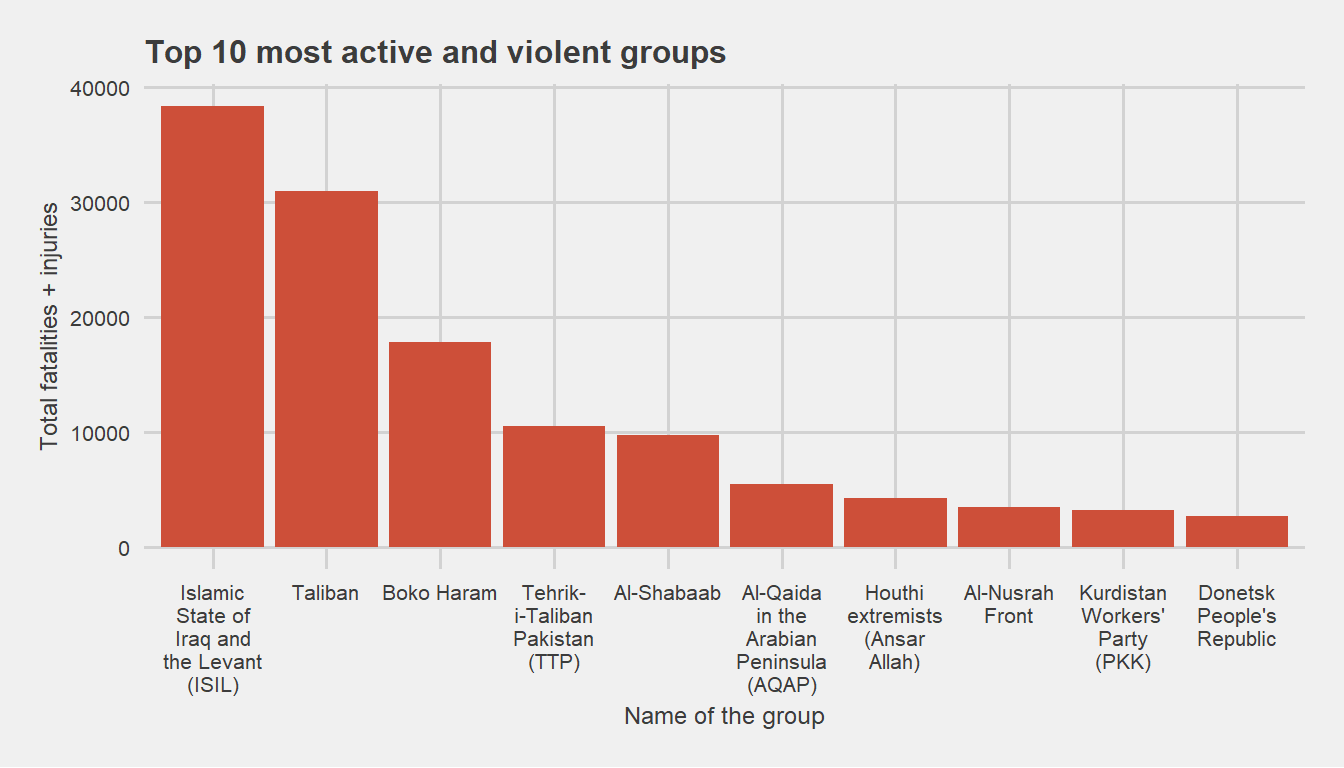
\includegraphics[width=1\linewidth]{thesis_files/figure-latex/unnamed-chunk-11-1} \caption{Top 10 most active and violent groups}\label{fig:unnamed-chunk-11}
\end{figure}
Based on a cumulative number of fatalities and injured people, we can
see that ISIL and Taliban, followed by Boko Haram are the most violent
groups that are currently active.

To better understand their activity over the period of time, we take a
look at attack frequency from each group.
\begin{Shaded}
\begin{Highlighting}[]
\NormalTok{tmp <-}\StringTok{ }\NormalTok{df }\OperatorTok\StringTok{ }
\StringTok{  }\KeywordTok{filter}\NormalTok{(group_name }\OperatorTok\StringTok{ }\NormalTok{top10_groups) }\OperatorTok\StringTok{ }
\StringTok{  }\KeywordTok{group_by}\NormalTok{(group_name, year) }\OperatorTok\StringTok{ }
\StringTok{  }\KeywordTok{summarise}\NormalTok{(}\DataTypeTok{total_attacks =} \KeywordTok{n}\NormalTok{())}
\end{Highlighting}
\end{Shaded}
\begin{figure}
\includegraphics[width=1\linewidth]{figure/heatmap_attack_t10} \caption{Attack frequency by Top 10 groups}\label{fig:unnamed-chunk-13}
\end{figure}
It's interesting to see that the majority of this most violent terrorist
groups (6 out of 10) were formed after 2006 only. Particularly, a number
of attacks from ISIL can be seen increasing rapidly within a shortest
period of time (4 years) and a gradual increase in attacks from Taliban
(reaching a peak at 1249 in the year 2015).

Attack characteristics for all 10 groups (cumulative) indicate Military
as the most frequent target (27.5\%) followed by civilians (27.3\%).
Similarly, Bombing/Explosions and Armed assault as a most frequent
attack tactics account for 70.4\% of all the attacks as shown in the
plots below.
\begin{figure}
\includegraphics[width=1\linewidth]{figure/heatmap_pie} \caption{Characteristics of top 10 groups}\label{fig:unnamed-chunk-14}
\end{figure}
\section{The major and minor
epicenters}\label{the-major-and-minor-epicenters}

The term ``Epicenter'' used here refers to the geographical location
that is impacted by terrorist incidents from top 10 groups as defined.
To examine the threat level from this groups by geographic location, I
use the cumulative sum of the number of people killed and a number of
people wounded as a measurement. Below is the code used to prepare the
data for this analysis.
\begin{Shaded}
\begin{Highlighting}[]
\NormalTok{tmp <-}\StringTok{ }\NormalTok{df }\OperatorTok\StringTok{ }
\StringTok{  }\KeywordTok{filter}\NormalTok{(group_name }\OperatorTok\StringTok{ }\NormalTok{top10_groups) }\OperatorTok
\StringTok{  }\KeywordTok{replace_na}\NormalTok{(}\KeywordTok{list}\NormalTok{(}\DataTypeTok{nkill =} \DecValTok{0}\NormalTok{, }\DataTypeTok{nwound =} \DecValTok{0}\NormalTok{)) }\OperatorTok\StringTok{ }
\StringTok{  }\KeywordTok{group_by}\NormalTok{(group_name, region, year, month) }\OperatorTok\StringTok{ }
\StringTok{  }\KeywordTok{filter}\NormalTok{(}\KeywordTok{if_else}\NormalTok{(part_of_multiple_attacks }\OperatorTok{==}\StringTok{ }\DecValTok{1}\NormalTok{, }
\NormalTok{                 nkill }\OperatorTok{==}\StringTok{ }\KeywordTok{max}\NormalTok{(nkill) }\OperatorTok{&}\StringTok{ }\NormalTok{nwound }\OperatorTok{==}\StringTok{ }\KeywordTok{max}\NormalTok{(nwound), }
\NormalTok{                 nkill }\OperatorTok{==}\StringTok{ }\NormalTok{nkill }\OperatorTok{&}\StringTok{ }\NormalTok{nwound }\OperatorTok{==}\StringTok{ }\NormalTok{nwound)) }\OperatorTok
\StringTok{  }\KeywordTok{ungroup}\NormalTok{() }\OperatorTok
\StringTok{  }\KeywordTok{distinct}\NormalTok{(group_name, region, country, year, month, nkill,}
\NormalTok{           nwound, part_of_multiple_attacks) }\OperatorTok
\StringTok{  }\KeywordTok{group_by}\NormalTok{(country, region) }\OperatorTok
\StringTok{  }\KeywordTok{summarise}\NormalTok{(}\DataTypeTok{attack_count =} \KeywordTok{n}\NormalTok{(), }
            \DataTypeTok{nkill_plus_nwound =} \KeywordTok{sum}\NormalTok{(nkill }\OperatorTok{+}\StringTok{ }\NormalTok{nwound))}
\end{Highlighting}
\end{Shaded}
\begin{Shaded}
\begin{Highlighting}[]
\CommentTok{# Threat level in four regions}
\NormalTok{tbl <-}\StringTok{ }\NormalTok{tmp }\OperatorTok\StringTok{ }
\StringTok{  }\KeywordTok{filter}\NormalTok{(region }\OperatorTok\StringTok{ }\KeywordTok{c}\NormalTok{(}\StringTok{"North America"}\NormalTok{, }\StringTok{"Eastern Europe"}\NormalTok{, }
                       \StringTok{"Central Asia"}\NormalTok{, }\StringTok{"Southeast Asia"}\NormalTok{))}
\end{Highlighting}
\end{Shaded}
\begin{table}[H]

\caption{\label{tab:unnamed-chunk-17}Threat level across regions}
\centering
\fontsize{12}{14}\selectfont
\begin{tabular}[t]{llrr}
\toprule
country & region & attack\_count & nkill\_plus\_nwound\\
\midrule
Georgia & Central Asia & 1 & 1\\
Turkmenistan & Central Asia & 1 & 5\\
Russia & Eastern Europe & 2 & 6\\
Ukraine & Eastern Europe & 170 & 2695\\
United States & North America & 2 & 2\\
\addlinespace
Indonesia & Southeast Asia & 1 & 2\\
Malaysia & Southeast Asia & 1 & 8\\
Philippines & Southeast Asia & 6 & 102\\
\bottomrule
\end{tabular}
\end{table}
We can see minor/ negligible threat level across North America and
Central Asia region, however, Ukraine turns out to be the major
epicenter in Eastern Europe region and poses high threat level.
Similarly, a low number of attacks but the high number of casualties and
injuries make Philippines minor epicenter within the Southeast Asia
region.

In the next plots, we use treemap to get a quick overview of the threat
level by regions. The area represents a number of attacks and color
represents cumulative fatalities and injuries.
\begin{Shaded}
\begin{Highlighting}[]
\NormalTok{tmp1 <-}\StringTok{ }\NormalTok{tmp }\OperatorTok\StringTok{ }
\StringTok{  }\KeywordTok{filter}\NormalTok{(region }\OperatorTok\StringTok{ }\KeywordTok{c}\NormalTok{(}\StringTok{"Western Europe"}\NormalTok{)) }
\end{Highlighting}
\end{Shaded}
\begin{figure}
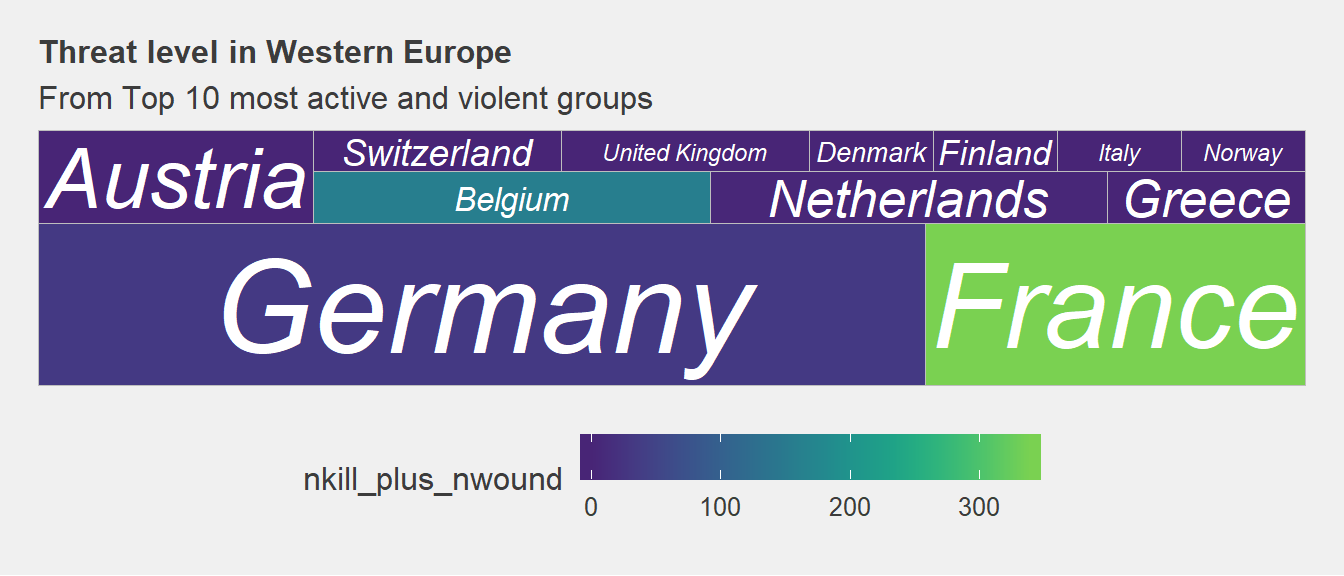
\includegraphics[width=1\linewidth]{thesis_files/figure-latex/unnamed-chunk-19-1} \caption{Threat level in Western Europe}\label{fig:unnamed-chunk-19}
\end{figure}
The situation in Western Europe represents the opposite of what we have
observed in Eastern Europe. Here we can see that terrorism from top ten
groups is spread across most the countries. While France facing the
biggest impact in terms of cumulative fatalities and injuries followed
by Belgium, we can also see that Germany is facing the highest number of
attacks.
\begin{table}[H]

\caption{\label{tab:unnamed-chunk-20}Threat level in Western Europe}
\centering
\fontsize{12}{14}\selectfont
\begin{tabular}[t]{llrr}
\toprule
country & region & attack\_count & nkill\_plus\_nwound\\
\midrule
Austria & Western Europe & 5 & 0\\
Belgium & Western Europe & 4 & 157\\
Denmark & Western Europe & 1 & 0\\
Finland & Western Europe & 1 & 1\\
France & Western Europe & 12 & 338\\
\addlinespace
Germany & Western Europe & 28 & 30\\
Greece & Western Europe & 2 & 0\\
Italy & Western Europe & 1 & 0\\
Netherlands & Western Europe & 4 & 4\\
Norway & Western Europe & 1 & 1\\
\addlinespace
Switzerland & Western Europe & 2 & 0\\
United Kingdom & Western Europe & 2 & 0\\
\bottomrule
\end{tabular}
\end{table}
Based on threat level, we can identify Germany and France as major
epicenters and Belgium as a minor epicenter in the Western Europe
region. It should be noted that the threat level in Ukraine alone is
almost 5 times higher than the threat level in the whole Western Europe
region.
\begin{Shaded}
\begin{Highlighting}[]
\NormalTok{tmp1 <-}\StringTok{ }\NormalTok{tmp }\OperatorTok\StringTok{ }
\StringTok{  }\KeywordTok{filter}\NormalTok{(region }\OperatorTok\StringTok{ }\KeywordTok{c}\NormalTok{(}\StringTok{"Middle East & North Africa"}\NormalTok{, }
                       \StringTok{"Sub-Saharan Africa"}\NormalTok{, }\StringTok{"South Asia"}\NormalTok{))}
\end{Highlighting}
\end{Shaded}
\begin{figure}
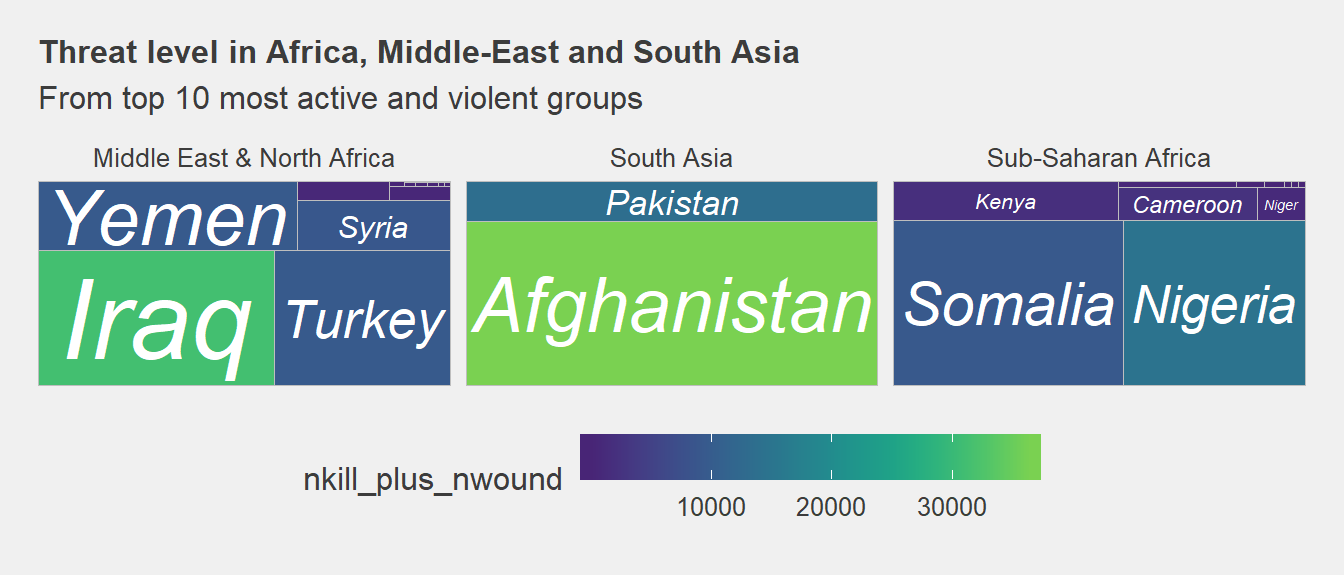
\includegraphics[width=1\linewidth]{thesis_files/figure-latex/unnamed-chunk-22-1} \caption{Threat level in Africa, Middle-East and South Asia}\label{fig:unnamed-chunk-22}
\end{figure}
\begin{table}[H]

\caption{\label{tab:unnamed-chunk-23}Threat level in Africa, Middle-East and South Asia}
\centering
\fontsize{9}{11}\selectfont
\begin{tabular}[t]{llrr}
\toprule
country & region & attack\_count & nkill\_plus\_nwound\\
\midrule
Afghanistan & South Asia & 3199 & 36364\\
Iraq & Middle East \& North Africa & 1480 & 31169\\
Nigeria & Sub-Saharan Africa & 746 & 14540\\
Pakistan & South Asia & 783 & 13192\\
Yemen & Middle East \& North Africa & 825 & 9334\\
\addlinespace
Turkey & Middle East \& North Africa & 1102 & 9259\\
Somalia & Sub-Saharan Africa & 942 & 8963\\
Syria & Middle East \& North Africa & 352 & 8776\\
Cameroon & Sub-Saharan Africa & 111 & 2170\\
Kenya & Sub-Saharan Africa & 213 & 1771\\
\addlinespace
Niger & Sub-Saharan Africa & 39 & 859\\
Saudi Arabia & Middle East \& North Africa & 81 & 509\\
Chad & Sub-Saharan Africa & 17 & 378\\
Lebanon & Middle East \& North Africa & 42 & 377\\
Ethiopia & Sub-Saharan Africa & 4 & 102\\
\addlinespace
Jordan & Middle East \& North Africa & 3 & 58\\
Tunisia & Middle East \& North Africa & 2 & 31\\
Djibouti & Sub-Saharan Africa & 1 & 20\\
Iran & Middle East \& North Africa & 1 & 11\\
Libya & Middle East \& North Africa & 2 & 7\\
\addlinespace
Tanzania & Sub-Saharan Africa & 1 & 7\\
Israel & Middle East \& North Africa & 1 & 4\\
Burkina Faso & Sub-Saharan Africa & 1 & 2\\
Egypt & Middle East \& North Africa & 1 & 2\\
Uganda & Sub-Saharan Africa & 3 & 1\\
West Bank and Gaza Strip & Middle East \& North Africa & 2 & 1\\
\bottomrule
\end{tabular}
\end{table}
From the plot and table above, we can see that all three regions are
heavily impacted. While Afghanistan facing the largest impact in terms
of fatalities and number of people injured followed by Iraq, we can also
see that the spread in Southeast Asia is limited to Pakistan and
Afghanistan only (similar to Eastern Europe).

In the case of Sub-Saharan Africa and the Middle East \& North Africa
region, we can see spread across many countries. We can also see many
countries with a low number of attacks but the relatively large number
of fatalities and injuries such as in Yemen, Niger, Nigeria, and Chad.
In a comparison to other regions, the cumulative sum of a number of
fatalities and injuries in Africa, Middle-East, and South Asia is more
than 9,000 in each of the top five highly impacted countries.

To further identify the epicenters by each group, let us narrow down our
analysis to the city level. For this analysis, I have set the threshold
for a cumulative number of fatalities and injuries to 100 and have
removed observations where the name of the city is unknown as shown in
the code chunk below:
\begin{Shaded}
\begin{Highlighting}[]
\CommentTok{#------------------------------------------}
\CommentTok{#Epicenters at city level per group}
\CommentTok{#------------------------------------------}
\NormalTok{tmp <-}\StringTok{ }\NormalTok{df }\OperatorTok\StringTok{ }
\StringTok{  }\KeywordTok{filter}\NormalTok{(group_name }\OperatorTok\StringTok{ }\NormalTok{top10_groups) }\OperatorTok
\StringTok{  }\KeywordTok{replace_na}\NormalTok{(}\KeywordTok{list}\NormalTok{(}\DataTypeTok{nkill =} \DecValTok{0}\NormalTok{, }\DataTypeTok{nwound =} \DecValTok{0}\NormalTok{)) }\OperatorTok\StringTok{ }
\StringTok{  }\KeywordTok{group_by}\NormalTok{(group_name, region, year, month) }\OperatorTok\StringTok{ }
\StringTok{  }\KeywordTok{filter}\NormalTok{(}\KeywordTok{if_else}\NormalTok{(part_of_multiple_attacks }\OperatorTok{==}\StringTok{ }\DecValTok{1}\NormalTok{, }
\NormalTok{                 nkill }\OperatorTok{==}\StringTok{ }\KeywordTok{max}\NormalTok{(nkill) }\OperatorTok{&}\StringTok{ }\NormalTok{nwound }\OperatorTok{==}\StringTok{ }\KeywordTok{max}\NormalTok{(nwound), }
\NormalTok{                 nkill }\OperatorTok{==}\StringTok{ }\NormalTok{nkill }\OperatorTok{&}\StringTok{ }\NormalTok{nwound }\OperatorTok{==}\StringTok{ }\NormalTok{nwound)) }\OperatorTok
\StringTok{  }\KeywordTok{ungroup}\NormalTok{() }\OperatorTok
\StringTok{  }\KeywordTok{distinct}\NormalTok{(group_name, region, country, city, year, month, }
\NormalTok{           nkill, nwound, part_of_multiple_attacks) }\OperatorTok
\StringTok{  }\KeywordTok{group_by}\NormalTok{(city, group_name) }\OperatorTok\StringTok{ }
\StringTok{  }\KeywordTok{summarise}\NormalTok{(}\DataTypeTok{attack_count =} \KeywordTok{n}\NormalTok{(), }
            \DataTypeTok{nkill_plus_nwound =} \KeywordTok{sum}\NormalTok{(nkill }\OperatorTok{+}\StringTok{ }\NormalTok{nwound)) }\OperatorTok
\StringTok{  }\KeywordTok{filter}\NormalTok{(nkill_plus_nwound }\OperatorTok{>=}\StringTok{ }\DecValTok{100} \OperatorTok{&}\StringTok{ }
\StringTok{         }\NormalTok{city }\OperatorTok{!=}\StringTok{ "Unknown"} \OperatorTok{&}\StringTok{ }
\StringTok{         }\NormalTok{city }\OperatorTok{!=}\StringTok{ "unknown"}\NormalTok{) }\OperatorTok
\StringTok{  }\KeywordTok{as.data.frame}\NormalTok{()}
\end{Highlighting}
\end{Shaded}
\begin{Shaded}
\begin{Highlighting}[]
\KeywordTok{glimpse}\NormalTok{(tmp)}
\end{Highlighting}
\end{Shaded}
\begin{verbatim}
Observations: 284
Variables: 4
$ city              <chr> "Abu Adh Dhuhur", "Abu Ghraib", "Abuja", "Ad...
$ group_name        <chr> "Al-Nusrah Front", "Islamic State of Iraq an...
$ attack_count      <int> 4, 13, 9, 55, 21, 7, 45, 29, 24, 14, 8, 29, ...
$ nkill_plus_nwound <dbl> 132, 103, 444, 261, 346, 110, 164, 383, 592,...
\end{verbatim}
From the prepared data, we can see that 284 cities are impacted by the
top 10 most active and violent groups. Next, we plot this data using
treemap where the size/area represents a number of attacks and color
represents the intensity of the cumulative sum of fatalities and
injuries.
\begin{figure}
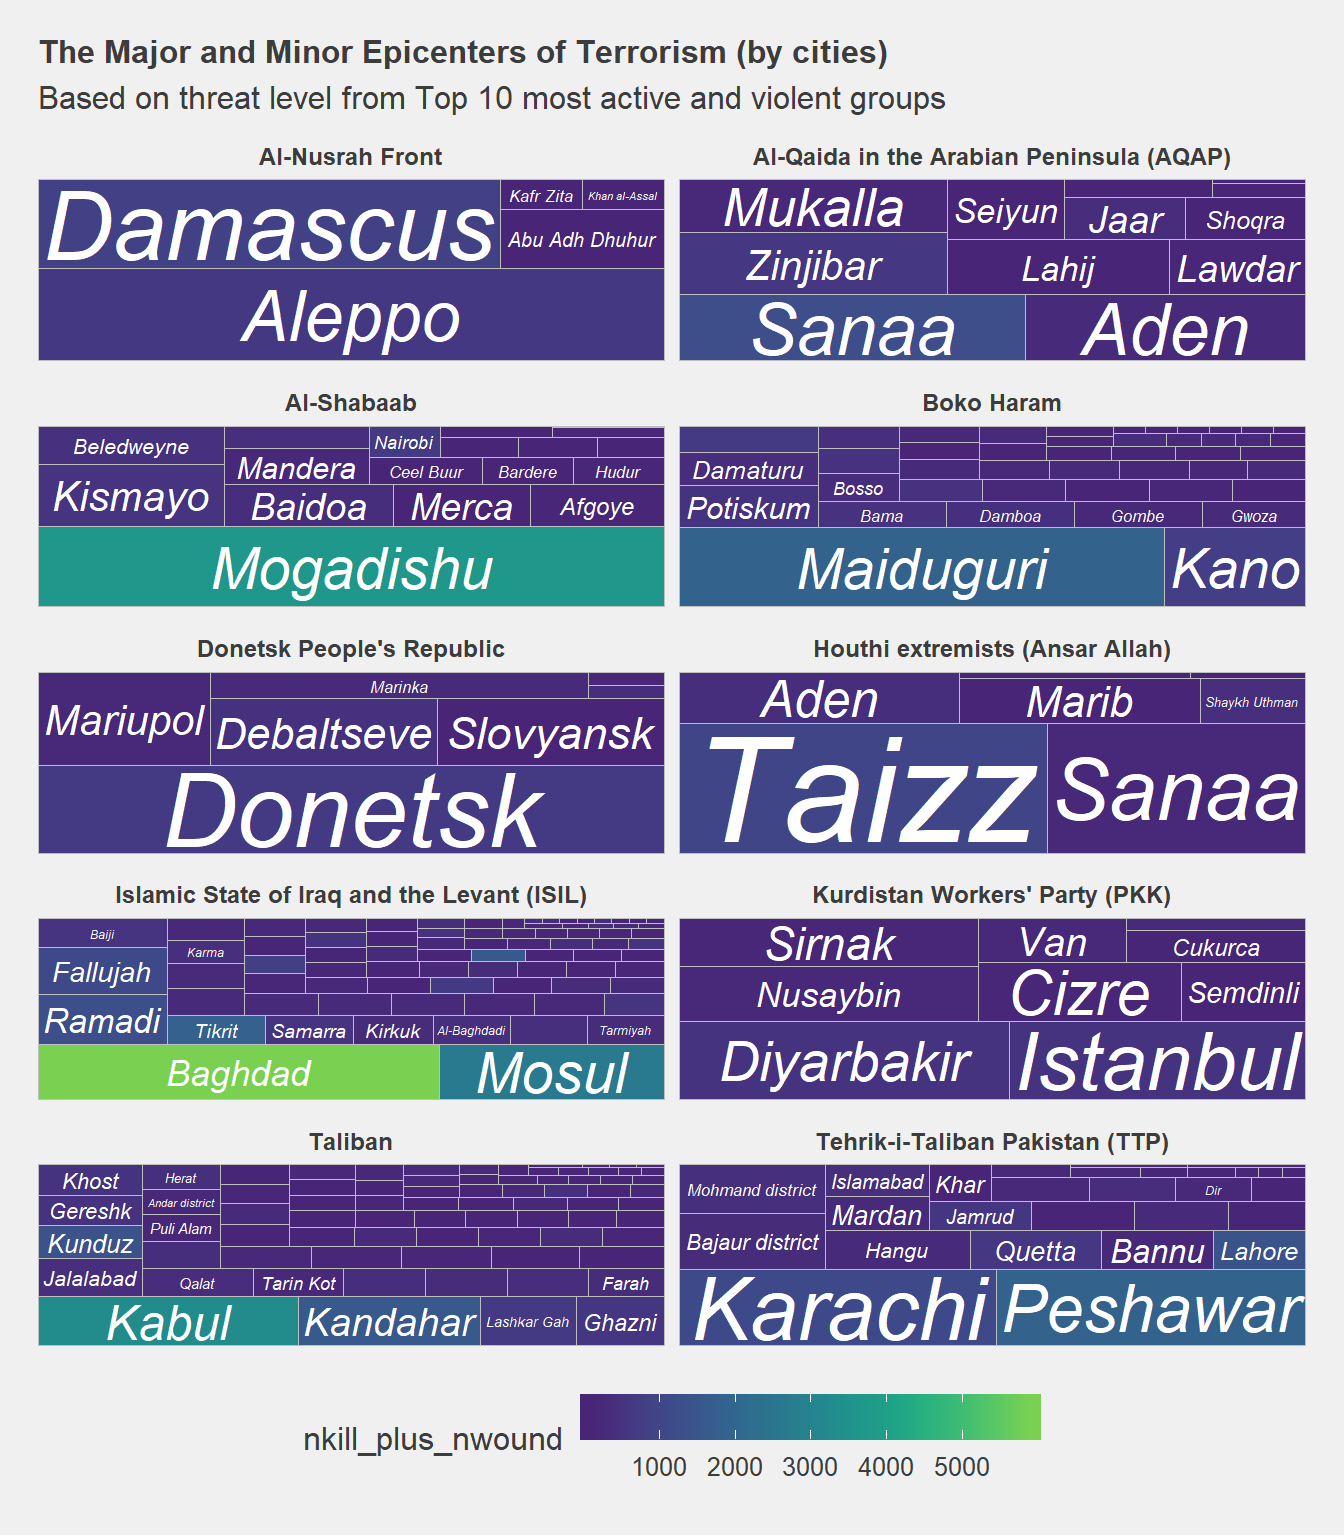
\includegraphics[width=1\linewidth]{thesis_files/figure-latex/unnamed-chunk-26-1} \caption{The Major and Minor Epicenters of Terrorism (by each group)}\label{fig:unnamed-chunk-26}
\end{figure}
We can see distinct characteristic among the groups in terms of spread.
For example, Al-Nusrah Front, Houthi Extremists and Donetsk People's
Republic groups have spread across 5 to 10 cities while having few major
epicenters. Whereas ISIL, Taliban and Boko Haram groups have spread
across many cities. In the case of ISIL, we can also see a relatively
large number of fatalities and injuries with a low number of attacks in
several cities.

To summarize, we identified the top 10 most lethal groups that are
active between 2010 to 2016 and examined their characteristics behind
attacks. We looked at the trend in the type of attack and a
corresponding number of attacks over the period of time, which up to
certain extent, indicates easy access to firearms and explosive devices
either through illegal arms trade or through undisclosed support from
powerful nation/s. We also examined pattern in target type, in which,
46.7\% attacks were targeted at the Military and Police category and
27.3\% attacks were intended toward civilians. Based on the threat level
from the top ten groups, we examined the geographical spread and
identified the hot spots where these groups are highly active.

\chapter{Statistical Hypothesis Testing}\label{hypothesis-testing}

In this chapter, first, we examine the strength of the relationship
between two numerical variables using Pearson correlation coefficient.
This way, we can get an idea of which variables have strong/weak and
positive/negative correlation with each other. In the second part, we
perform a hypothesis test between each of the top ten groups and the
number of fatalities to see which groups represent similarity and
differences. We use the data related to the top ten most active and
violent groups only.

\section{Data preparation}\label{data-preparation-1}
\begin{Shaded}
\begin{Highlighting}[]
\NormalTok{dfh <-}\StringTok{ }\NormalTok{df }\OperatorTok\StringTok{   }
\StringTok{  }\KeywordTok{filter}\NormalTok{(group_name }\OperatorTok\StringTok{ }\NormalTok{top10_groups) }\OperatorTok\StringTok{  }\CommentTok{# filter data by top 10 groups}
\StringTok{  }\KeywordTok{replace_na}\NormalTok{(}\KeywordTok{list}\NormalTok{(}\DataTypeTok{nkill =} \DecValTok{0}\NormalTok{, }\DataTypeTok{nwound =} \DecValTok{0}\NormalTok{))   }\CommentTok{# replace NAs}

\CommentTok{# Shorten lengthy group names}
\NormalTok{dfh}\OperatorTok{$}\NormalTok{group_name[dfh}\OperatorTok{$}\NormalTok{group_name }\OperatorTok{==}\StringTok{ "Kurdistan Workers' Party (PKK)"}\NormalTok{] <-}\StringTok{ "PKK"}
\NormalTok{dfh}\OperatorTok{$}\NormalTok{group_name[dfh}\OperatorTok{$}\NormalTok{group_name }\OperatorTok{==}\StringTok{ "Al-Qaida in the Arabian Peninsula (AQAP)"}\NormalTok{] <-}\StringTok{ "AQAP"}
\NormalTok{dfh}\OperatorTok{$}\NormalTok{group_name[dfh}\OperatorTok{$}\NormalTok{group_name }\OperatorTok{==}\StringTok{ "Houthi extremists (Ansar Allah)"}\NormalTok{] <-}\StringTok{ "Houthi_Extrm"}
\NormalTok{dfh}\OperatorTok{$}\NormalTok{group_name[dfh}\OperatorTok{$}\NormalTok{group_name }\OperatorTok{==}\StringTok{ "Tehrik-i-Taliban Pakistan (TTP)"}\NormalTok{] <-}\StringTok{ "TTP"}
\NormalTok{dfh}\OperatorTok{$}\NormalTok{group_name[dfh}\OperatorTok{$}\NormalTok{group_name }\OperatorTok{==}\StringTok{ "Al-Nusrah Front"}\NormalTok{] <-}\StringTok{ "Al-Nusrah"}
\NormalTok{dfh}\OperatorTok{$}\NormalTok{group_name[dfh}\OperatorTok{$}\NormalTok{group_name }\OperatorTok{==}\StringTok{ "Islamic State of Iraq and the Levant (ISIL)"}\NormalTok{] <-}\StringTok{"ISIL"}
\NormalTok{dfh}\OperatorTok{$}\NormalTok{group_name[dfh}\OperatorTok{$}\NormalTok{group_name }\OperatorTok{==}\StringTok{ "Donetsk People's Republic"}\NormalTok{] <-}\StringTok{ "Donetsk_PR"} 
\end{Highlighting}
\end{Shaded}
\section{Correlation test}\label{correlation-test}

We use pairwise complete observations method to compute correlation
coefficients for each pair of numerical variables.
\begin{Shaded}
\begin{Highlighting}[]
\CommentTok{#Extract numeric variables}
\NormalTok{tmp <-}\StringTok{ }\NormalTok{dfh }\OperatorTok
\StringTok{  }\KeywordTok{select}\NormalTok{(intl_ideological_attack, intl_logistical_attack, }
\NormalTok{         part_of_multiple_attacks, n_peace_keepers, net_migration, }
\NormalTok{         refugee_asylum, refugee_origin, gdp_per_capita, arms_import, }
\NormalTok{         arms_export, conflict_index, population, extended, }
\NormalTok{         nwound, nkill, suicide_attack, attack_success) }

\CommentTok{# get the correlation matrix}
\NormalTok{m <-}\StringTok{ }\KeywordTok{cor}\NormalTok{(tmp, }\DataTypeTok{use=}\StringTok{"pairwise.complete.obs"}\NormalTok{)}
\CommentTok{# Get rid of all non significant correlations}
\NormalTok{ctest <-}\StringTok{ }\KeywordTok{PairApply}\NormalTok{(tmp, }\DataTypeTok{symmetric=}\OtherTok{TRUE}\NormalTok{,}
                   \ControlFlowTok{function}\NormalTok{(x, y) }\KeywordTok{cor.test}\NormalTok{(x, y)}\OperatorTok{$}\NormalTok{p.value)}
\NormalTok{m[ctest }\OperatorTok{>}\StringTok{ }\FloatTok{0.05}\NormalTok{] <-}\StringTok{ }\OtherTok{NA}   \CommentTok{# Replace p value > 0.05 with NAs}
\KeywordTok{PlotWeb}\NormalTok{(m, }\DataTypeTok{lwd =} \KeywordTok{abs}\NormalTok{(m[}\KeywordTok{lower.tri}\NormalTok{(m)] }\OperatorTok{*}\StringTok{ }\DecValTok{10}\NormalTok{), }
        \DataTypeTok{main=}\StringTok{"Correlation Web Plot"}\NormalTok{, }
        \DataTypeTok{cex.lab =} \FloatTok{0.85}\NormalTok{, }\DataTypeTok{pt.bg =} \StringTok{"#f2f2f2"}\NormalTok{,}
        \DataTypeTok{args.legend =} \KeywordTok{list}\NormalTok{(}\DataTypeTok{x =} \StringTok{"bottomright"}\NormalTok{, }\DataTypeTok{cex =} \FloatTok{0.75}\NormalTok{, }\DataTypeTok{bty =} \StringTok{"0"}\NormalTok{, }
                           \DataTypeTok{title =} \StringTok{"Correlation"}\NormalTok{))}
\end{Highlighting}
\end{Shaded}
\begin{figure}
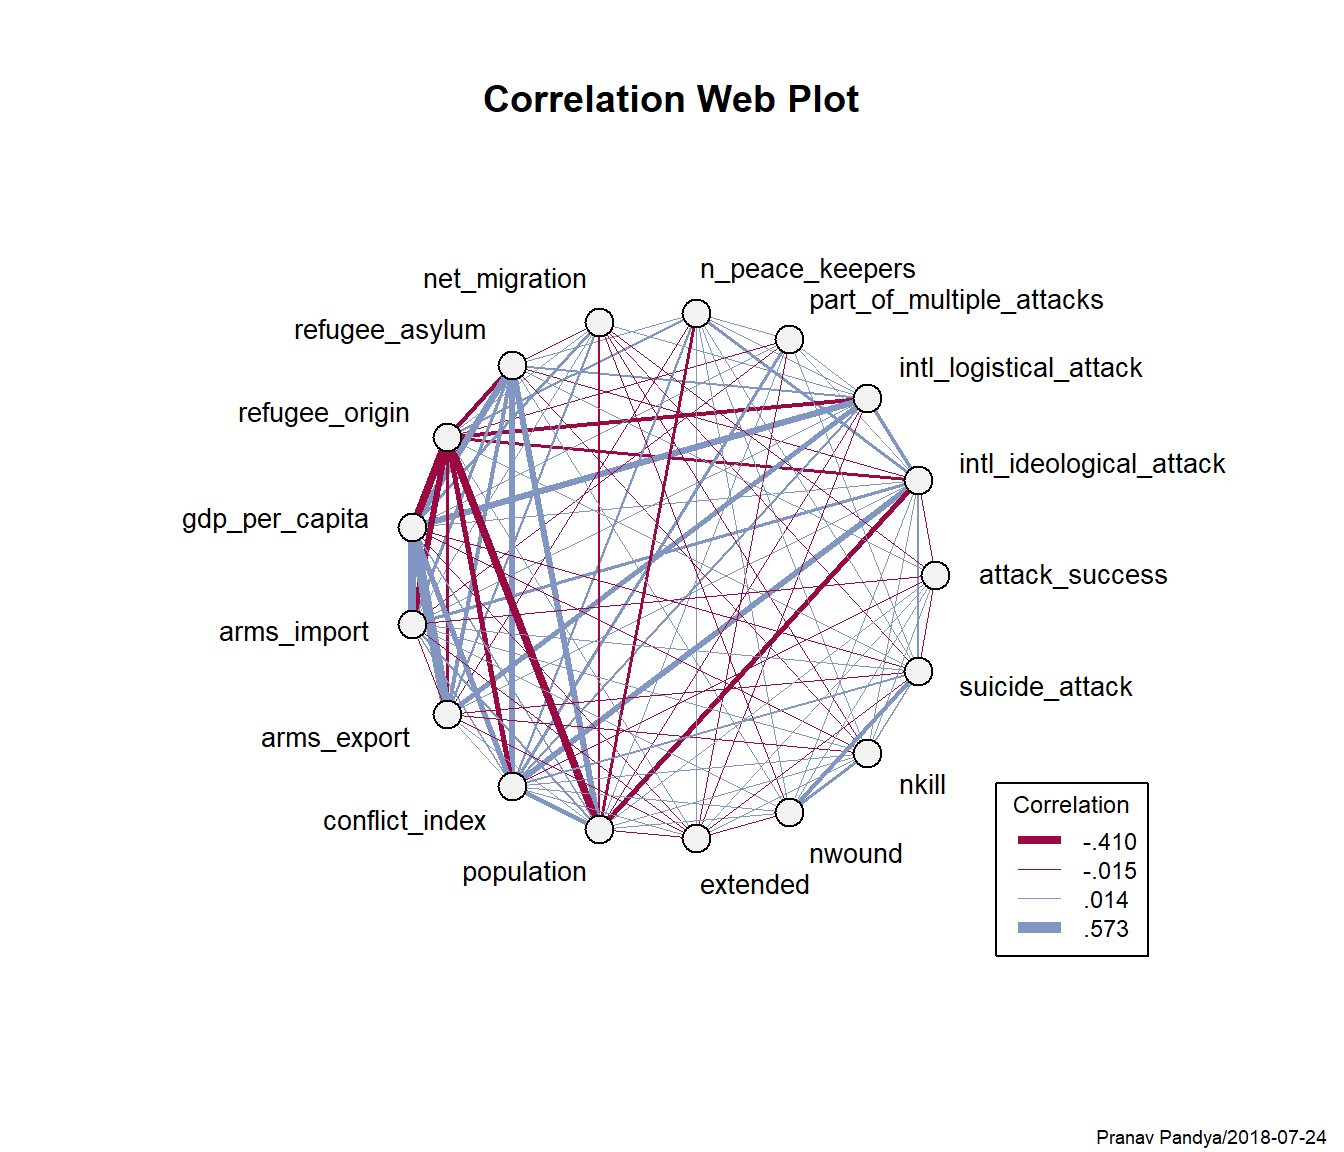
\includegraphics[width=1\linewidth]{thesis_files/figure-latex/unnamed-chunk-28-1} \caption{Correlation web plot}\label{fig:unnamed-chunk-28}
\end{figure}
In the plot above, line width between the nodes is used in proportion to
the correlation of two variables. To focus only on significant
correlations, I have replaced observations with p-value more than 0.05
with NA. Legend on the bottom right represents correlation coefficient
by line width and color depending on positive or negative linear
relationship. The variables on the left-hand side of the plot are
extracted from World Bank data (development indicators) and variables on
the right-hand side are from GTD.

Specifically, we are more interested in the relationship to the
variables on the right-hand side which will be used in time-series
forecasting and classification modeling as the target variable. For
example, a number of people wounded (nwound) variable has a positive
linear relationship with a suicide attack. The conflict index variable
shows a strong positive relationship with international ideological
attacks and minor positive relationship with a part of multiple attacks.
Overall, we can see that the majority of numerical variables shows a
relationship with each other.

\section{Hypothesis test: fatalities vs
groups}\label{hypothesis-test-fatalities-vs-groups}

The objective behind this hypothesis test is to determine whether or not
means of the top 10 groups with respect to average fatalities are same.
If at least one sample mean is different to others then we determine
which pair of groups are different.

\[
\large
\begin{aligned}
{H_0 : } & \text{ The means of the different groups are the same} \\
      &{(ISIL)} = {(Taliban)} = {(AQAP)} = {(PKK)} = \\
      &{(Al-Shabaab)} = {(TTP)} = {(Boko Haram)} =  \\
      &{(Al-Nusrah)} = {(Donetsk_PR)} = {(Houthi_Extrm)} \\ \\
H_a: & \text{ At least one sample mean is not equal to the others} 
\end{aligned}
\]

First, we use a box plot to examine distribution by quartiles for each
group.
\begin{figure}
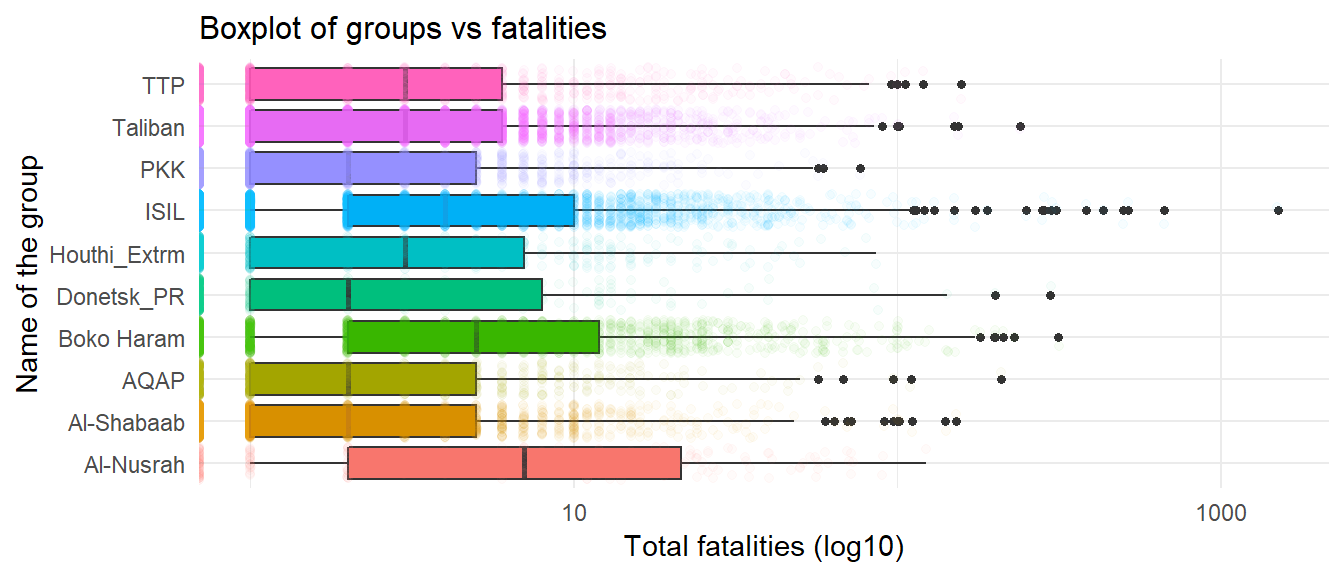
\includegraphics[width=1\linewidth]{thesis_files/figure-latex/unnamed-chunk-29-1} \caption{Boxplot: group vs fatalities}\label{fig:unnamed-chunk-29}
\end{figure}
In statistical terms, we have some extreme outliers i.e.~nkill
\textasciitilde{} 1500 in ISIL group so X axis is log transformed for
visualization purpose.

\subsection{ANOVA test}\label{anova-test}

The ANOVA model computes the residual variance and the variance between
sample means in order to calculate the F-statistic. This is the first
step to determine whether or not means are different in a pair of
groups.

\[
\large
\begin{aligned}
F-statistic = & (S^2_{between}\ / S^2_{within})
\end{aligned}
\]
\begin{Shaded}
\begin{Highlighting}[]
\CommentTok{#------------------------------------------}
\CommentTok{# Compute the analysis of variance (ANOVA)}
\CommentTok{#------------------------------------------}
\NormalTok{r.aov <-}\StringTok{ }\KeywordTok{aov}\NormalTok{(nkill }\OperatorTok{~}\StringTok{ }\NormalTok{group_name , }\DataTypeTok{data =}\NormalTok{ dfh)}

\CommentTok{# display result}
\KeywordTok{summary}\NormalTok{(r.aov)}
\end{Highlighting}
\end{Shaded}
\begin{verbatim}
               Df  Sum Sq Mean Sq F value              Pr(>F)    
group_name      9  111070   12341    40.7 <0.0000000000000002 ***
Residuals   21770 6597154     303                                
---
Signif. codes:  0 '***' 0.001 '**' 0.01 '*' 0.05 '.' 0.1 ' ' 1
\end{verbatim}
The model summary provides us F value and Pr(\textgreater{}F)
corresponding to the p-value of the test. As we can see that the p-value
is \textless{} 0.05, which means there are significant differences
between the groups. In other words, we reject the null hypothesis. From
this test, we identified that some of the group means are different
however we don't know which pair of groups have different means.

\subsection{PostHoc test}\label{posthoc-test}

PostHoc test is useful to determine where the differences occurred
between groups. For this test, we use several different methods for the
comparison purpose. This method can be classified as either conservative
or liberal approach. Conservative methods are considered to be robust
against committing Type I error as they use more stringent criterion for
statistical significance. First, we run the PostHoc test by comparing
results (p-value) from The Fisher LSD (Least Significant Different),
Scheffe and Dunn's (Bonferroni) test.
\begin{Shaded}
\begin{Highlighting}[]
\CommentTok{#------------------------------------------}
\CommentTok{# compare p-values for 3 methods}
\CommentTok{#------------------------------------------}
\NormalTok{posthoc1 <-}\StringTok{ }\KeywordTok{as.data.frame}\NormalTok{(}
  \KeywordTok{cbind}\NormalTok{(}
    \DataTypeTok{lsd=} \KeywordTok{PostHocTest}\NormalTok{(}
\NormalTok{      r.aov, }\DataTypeTok{method=}\StringTok{"lsd"}\NormalTok{)}\OperatorTok{$}\NormalTok{group_name[,}\StringTok{"pval"}\NormalTok{],     }\CommentTok{# The Fisher LSD}
    \DataTypeTok{scheffe=} \KeywordTok{PostHocTest}\NormalTok{(}
\NormalTok{      r.aov, }\DataTypeTok{method=}\StringTok{"scheffe"}\NormalTok{)}\OperatorTok{$}\NormalTok{group_name[,}\StringTok{"pval"}\NormalTok{], }\CommentTok{# Scheffe}
    \DataTypeTok{bonf=}\KeywordTok{PostHocTest}\NormalTok{(}
\NormalTok{      r.aov, }\DataTypeTok{method=}\StringTok{"bonf"}\NormalTok{)}\OperatorTok{$}\NormalTok{group_name[,}\StringTok{"pval"}\NormalTok{])    }\CommentTok{# Bonferroni}
\NormalTok{  ) }
\NormalTok{posthoc1 <-}\StringTok{ }\KeywordTok{rownames_to_column}\NormalTok{(posthoc1, }\DataTypeTok{var =} \StringTok{"Pair of groups"}\NormalTok{) }\OperatorTok\StringTok{ }
\StringTok{  }\KeywordTok{arrange}\NormalTok{(}\KeywordTok{desc}\NormalTok{(scheffe)) }
\end{Highlighting}
\end{Shaded}
\begin{table}[H]

\caption{\label{tab:unnamed-chunk-32}Posthoc test (lsd, scheffe, bonf)}
\centering
\fontsize{10}{12}\selectfont
\begin{tabular}[t]{lrrr}
\toprule
Pair of groups & lsd & scheffe & bonf\\
\midrule
Donetsk\_PR-Al-Shabaab & 0.9191 & 1.0000 & 1.0000\\
Houthi\_Extrm-Al-Shabaab & 0.7934 & 1.0000 & 1.0000\\
Houthi\_Extrm-Donetsk\_PR & 0.7797 & 1.0000 & 1.0000\\
Taliban-AQAP & 0.6811 & 1.0000 & 1.0000\\
PKK-Donetsk\_PR & 0.5800 & 1.0000 & 1.0000\\
\addlinespace
Houthi\_Extrm-AQAP & 0.4850 & 1.0000 & 1.0000\\
Donetsk\_PR-AQAP & 0.3615 & 0.9997 & 1.0000\\
PKK-Houthi\_Extrm & 0.3152 & 0.9994 & 1.0000\\
PKK-Al-Shabaab & 0.3021 & 0.9993 & 1.0000\\
AQAP-Al-Shabaab & 0.2561 & 0.9984 & 1.0000\\
\addlinespace
Taliban-Houthi\_Extrm & 0.1928 & 0.9954 & 1.0000\\
TTP-AQAP & 0.1508 & 0.9904 & 1.0000\\
Taliban-Donetsk\_PR & 0.1476 & 0.9898 & 1.0000\\
TTP-Taliban & 0.1253 & 0.9846 & 1.0000\\
Boko Haram-Al-Nusrah & 0.0851 & 0.9656 & 1.0000\\
\addlinespace
PKK-AQAP & 0.0610 & 0.9406 & 1.0000\\
TTP-Houthi\_Extrm & 0.0324 & 0.8694 & 1.0000\\
TTP-Donetsk\_PR & 0.0278 & 0.8481 & 1.0000\\
Taliban-Al-Shabaab & 0.0135 & 0.7301 & 0.6094\\
TTP-Al-Shabaab & 0.0024 & 0.4187 & 0.1088\\
\addlinespace
ISIL-Al-Nusrah & 0.0008 & 0.2574 & 0.0354\\
Taliban-PKK & 0.0005 & 0.2071 & 0.0226\\
ISIL-Boko Haram & 0.0002 & 0.1338 & 0.0097\\
TTP-PKK & 0.0002 & 0.1172 & 0.0076\\
TTP-ISIL & 0.0000 & 0.0072 & 0.0001\\
\addlinespace
TTP-Al-Nusrah & 0.0000 & 0.0006 & 0.0000\\
ISIL-AQAP & 0.0000 & 0.0000 & 0.0000\\
ISIL-Donetsk\_PR & 0.0000 & 0.0000 & 0.0000\\
AQAP-Al-Nusrah & 0.0000 & 0.0000 & 0.0000\\
Donetsk\_PR-Al-Nusrah & 0.0000 & 0.0000 & 0.0000\\
\addlinespace
Houthi\_Extrm-Al-Nusrah & 0.0000 & 0.0000 & 0.0000\\
Taliban-Al-Nusrah & 0.0000 & 0.0000 & 0.0000\\
ISIL-Houthi\_Extrm & 0.0000 & 0.0000 & 0.0000\\
TTP-Boko Haram & 0.0000 & 0.0000 & 0.0000\\
Al-Shabaab-Al-Nusrah & 0.0000 & 0.0000 & 0.0000\\
\addlinespace
PKK-Al-Nusrah & 0.0000 & 0.0000 & 0.0000\\
Donetsk\_PR-Boko Haram & 0.0000 & 0.0000 & 0.0000\\
Boko Haram-AQAP & 0.0000 & 0.0000 & 0.0000\\
Houthi\_Extrm-Boko Haram & 0.0000 & 0.0000 & 0.0000\\
Taliban-ISIL & 0.0000 & 0.0000 & 0.0000\\
\addlinespace
ISIL-Al-Shabaab & 0.0000 & 0.0000 & 0.0000\\
PKK-ISIL & 0.0000 & 0.0000 & 0.0000\\
Taliban-Boko Haram & 0.0000 & 0.0000 & 0.0000\\
Boko Haram-Al-Shabaab & 0.0000 & 0.0000 & 0.0000\\
PKK-Boko Haram & 0.0000 & 0.0000 & 0.0000\\
\bottomrule
\end{tabular}
\end{table}
The Fisher LSD (Least Significant Different) test is the most liberal in
all the PostHoc tests whereas the Scheffe test is the most conservative
and protects against Type I error. On the other hand, Dunn's
(Bonferroni) test is extremely conservative (Andri Signorell et mult.
al., 2018). Out of all the possible combination of pairs (45), 16 pair
of groups indicates p adj value \textgreater{} 0.9 based on the Scheffe
test. In statistical terms, it means 16 pairs of groups as shown in the
table above have non-significantly different means in a number of
fatalities.

Next, we use Tukey HSD (Honestly Significant Difference) method which is
the most common and preferred method.
\begin{Shaded}
\begin{Highlighting}[]
\CommentTok{#---------------------------------------}
\CommentTok{# PostHoc Test with Tukey HSD method}
\CommentTok{#---------------------------------------}
\CommentTok{#extract only p-values by setting conf.level to NA}
\NormalTok{hsd <-}\StringTok{ }\KeywordTok{PostHocTest}\NormalTok{(r.aov, }\DataTypeTok{method =} \StringTok{"hsd"}\NormalTok{, }\DataTypeTok{conf.level=}\OtherTok{NA}\NormalTok{)}
\CommentTok{# convert to data frame and round off to 3 digits}
\NormalTok{hsd <-}\StringTok{ }\KeywordTok{as.data.frame}\NormalTok{(}\KeywordTok{do.call}\NormalTok{(rbind, hsd)) }\OperatorTok\StringTok{ }\KeywordTok{round}\NormalTok{(}\DecValTok{3}\NormalTok{)}
\end{Highlighting}
\end{Shaded}
\begin{table}[H]

\caption{\label{tab:unnamed-chunk-34}PostHoc test with Tukey HSD for pair of groups}
\centering
\fontsize{7}{9}\selectfont
\begin{tabular}[t]{lrrrrrrrrr}
\toprule
  & Al-Nusrah & Al-Shabaab & AQAP & Boko Haram & Donetsk\_PR & Houthi\_Extrm & ISIL & PKK & Taliban\\
\midrule
Al-Shabaab & 0.000 & NA & NA & NA & NA & NA & NA & NA & NA\\
AQAP & 0.000 & 0.981 & NA & NA & NA & NA & NA & NA & NA\\
Boko Haram & 0.783 & 0.000 & 0.000 & NA & NA & NA & NA & NA & NA\\
Donetsk\_PR & 0.000 & 1.000 & 0.996 & 0.000 & NA & NA & NA & NA & NA\\
Houthi\_Extrm & 0.000 & 1.000 & 1.000 & 0.000 & 1.000 & NA & NA & NA & NA\\
\addlinespace
ISIL & 0.027 & 0.000 & 0.000 & 0.008 & 0.000 & 0.000 & NA & NA & NA\\
PKK & 0.000 & 0.990 & 0.687 & 0.000 & 1.000 & 0.992 & 0 & NA & NA\\
Taliban & 0.000 & 0.285 & 1.000 & 0.000 & 0.912 & 0.953 & 0 & 0.018 & NA\\
TTP & 0.000 & 0.073 & 0.916 & 0.000 & 0.457 & 0.499 & 0 & 0.007 & 0.879\\
\bottomrule
\end{tabular}
\end{table}
\subsection{Interpretation}\label{interpretation}

The pairs of groups with adj p-value near or equals to 1 represents
non-significantly different means in a number of fatalities such as Boko
Haram - Al-Nusrah, Al-Qaida in Arabian Peninsula (AQAP)- Al-Shabaab,
Houthi Extremist- PKK, Taliban- Tehrik-i-Taliban etc.

Similarly, a pair of groups with adjusted p-value near zero indicates
significantly different means in a number of fatalities such as pairs of
ISIL with all the remaining groups, Taliban - Al-Nusrah, PKK - Boko
Haram, Donetsk\_PR - Al-Nusrah etc.

\chapter{Pattern discovery}\label{pattern-discovery}

This part of the analysis is based on unsupervised machine learning
algorithm and makes use of association rules to discover patterns in
terrorist incidents from Islamic State, Taliban and Boko Haram group
that were identified in top ten most active and violent groups.

Mining of association rules is a widely used method in retail and
eCommerce environment and commonly known as Market Basket Analysis using
Apriori algorithm. The logic behind this approach is that if a customer
buys a certain group of products then they are more or less likely to
buy another group of products (Karthiyayini \& Balasubramanian, 2016).

\textbf{Pseudocode of the Apriori algorithm:} (minimal version\footnote{\url{https://en.wikipedia.org/wiki/Apriori_algorithm}})

\[
\begin{aligned}
& \mathrm{Apriori}(T,\epsilon)\\
&\qquad L_1 \gets \{ \mathrm{large~1-item sets} \} \\
&\qquad k \gets 2\\
&\qquad \mathrm{\textbf{while}}~ L_{k-1} \neq \ \emptyset \\
&\qquad \qquad C_k \gets \{ a \cup \{b\} \mid a \in L_{k-1} \land b \not \in a \} - \{ c \mid \{ s \mid s \subseteq c \land |s| = k-1 \} \nsubseteq L_{k-1} \}\\
&\qquad \qquad \mathrm{\textbf{for}~transactions}~t \in T\\
&\qquad \qquad\qquad D_t \gets \{ c \mid c \in C_k \land c \subseteq t \} \\
&\qquad \qquad\qquad \mathrm{\textbf{for}~candidates}~c \in D_t\\
&\qquad \qquad\qquad\qquad \mathit{count}[c] \gets \mathit{count}[c]+1\\
&\qquad \qquad L_k \gets \{ c \mid c \in C_k \land ~ \mathit{count}[c] \geq \epsilon \}\\
&\qquad \qquad k \gets k+1\\
&\qquad \mathrm{\textbf{return}}~\bigcup_k L_k
\end{aligned}
\]

As the goal of this algorithm is to determine the set of frequent items
among the candidates, this methodology can also be applied to discover
patterns within the terrorism context. The idea is to understand attack
habits from terrorist groups by finding association and correlation
between different attacks that were carried out in the past. It's
important to note that output from this algorithm is a list of
association rules (frequent patterns) and provides descriptive analysis
only. The real value of such unsupervised learning is in the insights we
can take away from the algorithm's finding.

\section{Data preparation}\label{data-preparation-2}

For this analysis, I have chosen specific variables that are not highly
correlated with chosen groups i.e.~target type, weapon type, attack
type, suicide attack and a number of fatalities while excluding the
observations where the value is ``Unknown''.
\begin{Shaded}
\begin{Highlighting}[]
\NormalTok{tmp <-}\StringTok{ }\NormalTok{dfh }\OperatorTok
\StringTok{  }\KeywordTok{select}\NormalTok{(group_name, target_type, weapon_type, attack_type, suicide_attack, nkill) }\OperatorTok
\StringTok{  }\KeywordTok{filter}\NormalTok{(target_type }\OperatorTok{!=}\StringTok{ "Unknown"} \OperatorTok{&}\StringTok{ }\NormalTok{target_type }\OperatorTok{!=}\StringTok{ "Other"} \OperatorTok{&}\StringTok{ }
\StringTok{         }\NormalTok{weapon_type }\OperatorTok{!=}\StringTok{ "Unknown"} \OperatorTok{&}\StringTok{ }\NormalTok{attack_type }\OperatorTok{!=}\StringTok{ "Unknown"}\NormalTok{) }\OperatorTok
\StringTok{  }\KeywordTok{mutate}\NormalTok{(}\DataTypeTok{nkill =} \KeywordTok{if_else}\NormalTok{(nkill }\OperatorTok{==}\StringTok{ }\DecValTok{0}\NormalTok{, }\StringTok{"0"}\NormalTok{,}
                 \KeywordTok{if_else}\NormalTok{(nkill }\OperatorTok{>=}\StringTok{ }\DecValTok{1} \OperatorTok{&}\StringTok{ }\NormalTok{nkill }\OperatorTok{<=}\StringTok{ }\DecValTok{5}\NormalTok{, }\StringTok{"1 to 5"}\NormalTok{,}
                 \KeywordTok{if_else}\NormalTok{(nkill }\OperatorTok{>}\StringTok{ }\DecValTok{5} \OperatorTok{&}\StringTok{ }\NormalTok{nkill }\OperatorTok{<=}\StringTok{ }\DecValTok{10}\NormalTok{, }\StringTok{"6 to 10"}\NormalTok{,}
                 \KeywordTok{if_else}\NormalTok{(nkill }\OperatorTok{>}\StringTok{ }\DecValTok{10} \OperatorTok{&}\StringTok{ }\NormalTok{nkill }\OperatorTok{<=}\StringTok{ }\DecValTok{50}\NormalTok{, }\StringTok{"11 to 50"}\NormalTok{,  }\StringTok{"more than 50"}\NormalTok{)))))}

\CommentTok{#shorten lengthy names for visualization purpose}
\NormalTok{tmp}\OperatorTok{$}\NormalTok{weapon_type[}
\NormalTok{  tmp}\OperatorTok{$}\NormalTok{weapon_type }\OperatorTok{==}\StringTok{ "Explosives/Bombs/Dynamite"}\NormalTok{] <-}\StringTok{ "Explosives"}
\NormalTok{tmp}\OperatorTok{$}\NormalTok{attack_type[}
\NormalTok{  tmp}\OperatorTok{$}\NormalTok{attack_type }\OperatorTok{==}\StringTok{ "Facility/Infrastructure Attack"}\NormalTok{] <-}\StringTok{ "Facility/Infra."}
\NormalTok{tmp}\OperatorTok{$}\NormalTok{target_type[}
\NormalTok{  tmp}\OperatorTok{$}\NormalTok{target_type }\OperatorTok{==}\StringTok{ "Private Citizens & Property"}\NormalTok{] <-}\StringTok{ "Civilians"}
\NormalTok{tmp}\OperatorTok{$}\NormalTok{target_type[}
\NormalTok{  tmp}\OperatorTok{$}\NormalTok{target_type }\OperatorTok{==}\StringTok{ "Terrorists/Non-State Militia"}\NormalTok{] <-}\StringTok{ "Non-State Militia"}
\NormalTok{tmp}\OperatorTok{$}\NormalTok{target_type[}
\NormalTok{  tmp}\OperatorTok{$}\NormalTok{target_type }\OperatorTok{==}\StringTok{ "Religious Figures/Institutions"}\NormalTok{] <-}\StringTok{ "Religious Figures"}

\CommentTok{#convert everything to factor}
\NormalTok{tmp[] <-}\StringTok{ }\KeywordTok{lapply}\NormalTok{(tmp, factor)}
\KeywordTok{str}\NormalTok{(tmp)}
\end{Highlighting}
\end{Shaded}
\begin{verbatim}
'data.frame':   18006 obs. of  6 variables:
 $ group_name    : Factor w/ 10 levels "Al-Nusrah","Al-Shabaab",..: 8 8 8 8 8 8 8 8 8 8 ...
 $ target_type   : Factor w/ 19 levels "Airports & Aircraft",..: 10 10 2 3 3 3 3 6 3 3 ...
 $ weapon_type   : Factor w/ 8 levels "Chemical","Explosives",..: 2 3 3 3 3 3 3 3 3 3 ...
 $ attack_type   : Factor w/ 8 levels "Armed Assault",..: 3 3 4 3 3 1 1 2 1 1 ...
 $ suicide_attack: Factor w/ 2 levels "0","1": 1 1 1 1 1 1 1 1 1 1 ...
 $ nkill         : Factor w/ 5 levels "0","1 to 5","11 to 50",..: 2 2 1 3 4 3 2 2 1 4 ...
\end{verbatim}
\section{Explanation of key terms}\label{explanation-of-key-terms}

The Apriori algorithm has three main measures namely support, confidence
and lift. These three measures are used to decide the relative strength
of the rules. In the model parameters, we set RHS to the chosen group
and LHS refers to a frequent pattern that is observed.

\textbf{Support} indicates how interesting a pattern is. In the
algorithm configuration (params), I have set the threshold to 0.001
which means a pattern must have appeared at least 0.001 * nrow(tmp) = 18
times.

\textbf{Confidence} value i.e 0.5 (set as a threshold in model params)
means that in order to be included in the results, the rule has to be
correct at least 50 percent of the time. This is particularly helpful to
eliminate the unreliable rules.

\textbf{Lift} indicates probability (support) of the itemset (pattern)
over the product of the probabilities of all items in the itemset
(Hahsler et al., 2018).

In general, high confidence and good lift are the standard measures to
evaluate the importance of a particular rule/ association however not
all the rules are useful. This rules normally fall into three categories
i.e.~actionable, trivial(useless) and inexplicable (Klimberg \&
McCullough, 2017). Example of the useless rule can be an association
that is obvious and thus not worth mentioning.

\section{Islamic State (ISIL)}\label{islamic-state-isil}

\subsection{Apriori model summary}\label{apriori-model-summary}
\begin{Shaded}
\begin{Highlighting}[]
\CommentTok{# set params}
\NormalTok{params <-}\StringTok{ }\KeywordTok{list}\NormalTok{(}\DataTypeTok{support =} \FloatTok{0.001}\NormalTok{, }\DataTypeTok{confidence =} \FloatTok{0.5}\NormalTok{, }\DataTypeTok{minlen =} \DecValTok{2}\NormalTok{)}
\NormalTok{group_ISIL <-}\StringTok{ }\KeywordTok{list}\NormalTok{(}\DataTypeTok{rhs=}\StringTok{'group_name=ISIL'}\NormalTok{, }\DataTypeTok{default=}\StringTok{"lhs"}\NormalTok{)}

\CommentTok{# apriori model}
\NormalTok{rules <-}\StringTok{ }\KeywordTok{apriori}\NormalTok{(}\DataTypeTok{data =}\NormalTok{ tmp, }\DataTypeTok{parameter=}\NormalTok{ params, }\DataTypeTok{appearance =}\NormalTok{ group_ISIL)}
\end{Highlighting}
\end{Shaded}
\begin{verbatim}
Apriori

Parameter specification:
 confidence minval smax arem  aval originalSupport maxtime support minlen
        0.5    0.1    1 none FALSE            TRUE       5   0.001      2
 maxlen target   ext
     10  rules FALSE

Algorithmic control:
 filter tree heap memopt load sort verbose
    0.1 TRUE TRUE  FALSE TRUE    2    TRUE

Absolute minimum support count: 18 

set item appearances ...[1 item(s)] done [0.00s].
set transactions ...[52 item(s), 18006 transaction(s)] done [0.01s].
sorting and recoding items ... [48 item(s)] done [0.00s].
creating transaction tree ... done [0.00s].
checking subsets of size 1 2 3 4 5 6 done [0.00s].
writing ... [51 rule(s)] done [0.00s].
creating S4 object  ... done [0.00s].
\end{verbatim}
In the model summary, we can see that the Absolute minimum support count
is 18 which means the pattern needs to appear at least 18 times in order
to be included. We have set this threshold with support value as
explained previously. Out of all the patterns, the model is able to find
51 association rules for the ISIL group. We further remove the rules
that may be redundant before starting our analysis.

\subsection{Top 5 patterns (ISIL)}\label{top-5-patterns-isil}
\begin{Shaded}
\begin{Highlighting}[]
\NormalTok{rules <-}\StringTok{ }\NormalTok{rules[}\OperatorTok{!}\KeywordTok{is.redundant}\NormalTok{(rules)] }\CommentTok{# Remove redundant rules if any }
\CommentTok{# Extract top 5 patterns based on confidence}
\NormalTok{subrules <-}\StringTok{ }\KeywordTok{head}\NormalTok{(}\KeywordTok{sort}\NormalTok{(rules, }\DataTypeTok{by=}\StringTok{"confidence"}\NormalTok{), }\DecValTok{5}\NormalTok{)}
\end{Highlighting}
\end{Shaded}
\begin{verbatim}
    lhs                               rhs                support confidence  lift count
[1] {weapon_type=Chemical,                                                             
     attack_type=Bombing/Explosion} : {group_name=ISIL} 0.001055     0.9048 4.869    19
[2] {target_type=Non-State Militia,                                                    
     attack_type=Bombing/Explosion,                                                    
     nkill=6 to 10}                 : {group_name=ISIL} 0.001055     0.7308 3.933    19
[3] {target_type=Non-State Militia,                                                    
     attack_type=Bombing/Explosion,                                                    
     suicide_attack=1}              : {group_name=ISIL} 0.003443     0.6526 3.512    62
[4] {target_type=Military,                                                             
     suicide_attack=1,                                                                 
     nkill=11 to 50}                : {group_name=ISIL} 0.007997     0.6457 3.475   144
[5] {target_type=Non-State Militia,                                                    
     suicide_attack=1}              : {group_name=ISIL} 0.003499     0.6238 3.357    63
\end{verbatim}
From the top five patterns based on confidence, we can see that the use
of chemical weapon turns out to be the most frequent pattern with
relatively high lift value. It is also interesting to see that attacks
on other terrorists (non state militia) are observed in 3 out of top 5
patterns.
\begin{figure}
\includegraphics[width=1\linewidth]{thesis_files/figure-latex/unnamed-chunk-38-1} \caption{Association rules in ISIL group}\label{fig:unnamed-chunk-38}
\end{figure}
The plot shown above represents all the discovered patterns (after
removing redundant rules). We can see that majority of discovered rules
are between 0.5 to 0.7 confidence while two rules with high support and
both indicating an attack on the military with a suicide attack.

\subsection{Network graph (ISIL)}\label{network-graph-isil}

The network graph shown below summarizes how things are related and
interconnected with each other and describes the habits of the ISIL
group.
\begin{figure}
\includegraphics[width=1\linewidth]{thesis_files/figure-latex/unnamed-chunk-40-1} \caption{Network graph of discovered patterns- ISIL group}\label{fig:unnamed-chunk-40}
\end{figure}
\section{Taliban}\label{taliban}

\subsection{Apriori model summary}\label{apriori-model-summary-1}
\begin{Shaded}
\begin{Highlighting}[]
\CommentTok{#---------------------------------------}
\CommentTok{#Apriori model on Taliban group}
\CommentTok{#---------------------------------------}
\NormalTok{params <-}\StringTok{ }\KeywordTok{list}\NormalTok{(}\DataTypeTok{support =} \FloatTok{0.001}\NormalTok{, }\DataTypeTok{confidence =} \FloatTok{0.5}\NormalTok{, }\DataTypeTok{minlen =} \DecValTok{2}\NormalTok{)}
\NormalTok{group_Taliban <-}\StringTok{ }\KeywordTok{list}\NormalTok{(}\DataTypeTok{rhs=}\StringTok{'group_name=Taliban'}\NormalTok{, }\DataTypeTok{default=}\StringTok{"lhs"}\NormalTok{)}
\NormalTok{rules <-}\StringTok{ }\KeywordTok{apriori}\NormalTok{(}\DataTypeTok{data =}\NormalTok{ tmp, }
                 \DataTypeTok{parameter=}\NormalTok{ params, }
                 \DataTypeTok{appearance =}\NormalTok{ group_Taliban)}
\end{Highlighting}
\end{Shaded}
\begin{verbatim}
Apriori

Parameter specification:
 confidence minval smax arem  aval originalSupport maxtime support minlen
        0.5    0.1    1 none FALSE            TRUE       5   0.001      2
 maxlen target   ext
     10  rules FALSE

Algorithmic control:
 filter tree heap memopt load sort verbose
    0.1 TRUE TRUE  FALSE TRUE    2    TRUE

Absolute minimum support count: 18 

set item appearances ...[1 item(s)] done [0.00s].
set transactions ...[52 item(s), 18006 transaction(s)] done [0.00s].
sorting and recoding items ... [48 item(s)] done [0.00s].
creating transaction tree ... done [0.00s].
checking subsets of size 1 2 3 4 5 6 done [0.00s].
writing ... [139 rule(s)] done [0.00s].
creating S4 object  ... done [0.00s].
\end{verbatim}
From the model summary, we can see that the algorithm is able to
identify 139 rules within the set threshold as defined in model
parameters. However, it is possible that many rules may be redundant so
we eliminate those rules.

\subsection{Top 5 patterns (Taliban)}\label{top-5-patterns-taliban}
\begin{Shaded}
\begin{Highlighting}[]
\CommentTok{#---------------------------------------}
\CommentTok{#Remove redundant rules if any}
\CommentTok{#---------------------------------------}
\NormalTok{rules <-}\StringTok{ }\NormalTok{rules[}\OperatorTok{!}\KeywordTok{is.redundant}\NormalTok{(rules)]}

\CommentTok{# Extract top 5 patterns based on confidence}
\NormalTok{subrules <-}\StringTok{ }\KeywordTok{head}\NormalTok{(}\KeywordTok{sort}\NormalTok{(rules, }\DataTypeTok{by=}\StringTok{"confidence"}\NormalTok{), }\DecValTok{5}\NormalTok{)}
\end{Highlighting}
\end{Shaded}
\pagebreak
\begin{verbatim}
    lhs                             rhs                   support confidence  lift count
[1] {weapon_type=Chemical,                                                              
     attack_type=Unarmed Assault} : {group_name=Taliban} 0.001222     0.8800 2.945    22
[2] {target_type=Police,                                                                
     weapon_type=Firearms,                                                              
     attack_type=Armed Assault,                                                         
     nkill=11 to 50}              : {group_name=Taliban} 0.004998     0.8257 2.763    90
[3] {target_type=Police,                                                                
     weapon_type=Firearms,                                                              
     nkill=6 to 10}               : {group_name=Taliban} 0.010163     0.8243 2.759   183
[4] {target_type=Police,                                                                
     weapon_type=Incendiary,                                                            
     attack_type=Facility/Infra.,                                                       
     nkill=0}                     : {group_name=Taliban} 0.001999     0.8000 2.677    36
[5] {target_type=Police,                                                                
     weapon_type=Firearms,                                                              
     nkill=11 to 50}              : {group_name=Taliban} 0.005665     0.7969 2.667   102
\end{verbatim}
From the top five patterns above, we can see that the use of chemical
weapon indicates the highest confidence and lift value. This was also
the case in the ISIL group. It is also observed that police is the most
common target in the incidents involving the use of firearms and
resulting fatalities between 11 to 50.
\begin{figure}
\includegraphics[width=1\linewidth]{thesis_files/figure-latex/unnamed-chunk-44-1} \caption{Association Rules in Taliban group}\label{fig:unnamed-chunk-44}
\end{figure}
From the plot above, we can identify many interesting patterns with
confidence above 0.55 with high support such as attacks on NGO and
government officials however most patterns indicate an attack on police
only. Let us have a detailed look at all the patterns with network
graph.

\subsection{Network graph (Taliban)}\label{network-graph-taliban}
\begin{figure}
\includegraphics[width=1\linewidth]{thesis_files/figure-latex/unnamed-chunk-46-1} \caption{Network graph of discovered patterns- Taliban group}\label{fig:unnamed-chunk-46}
\end{figure}
\section{Boko Haram}\label{boko-haram}

\subsection{Apriori model summary}\label{apriori-model-summary-2}
\begin{Shaded}
\begin{Highlighting}[]
\NormalTok{params <-}\StringTok{ }\KeywordTok{list}\NormalTok{(}\DataTypeTok{support =} \FloatTok{0.001}\NormalTok{, }\DataTypeTok{confidence =} \FloatTok{0.5}\NormalTok{, }\DataTypeTok{minlen =} \DecValTok{2}\NormalTok{)}
\NormalTok{group_Boko_Haram <-}\StringTok{ }\KeywordTok{list}\NormalTok{(}\DataTypeTok{rhs=}\StringTok{'group_name=Boko Haram'}\NormalTok{, }\DataTypeTok{default=}\StringTok{"lhs"}\NormalTok{)}
\NormalTok{rules <-}\StringTok{ }\KeywordTok{apriori}\NormalTok{(}\DataTypeTok{data =}\NormalTok{ tmp, }\DataTypeTok{parameter=}\NormalTok{ params, }\DataTypeTok{appearance =}\NormalTok{ group_Boko_Haram)}
\end{Highlighting}
\end{Shaded}
\begin{verbatim}
Apriori

Parameter specification:
 confidence minval smax arem  aval originalSupport maxtime support minlen
        0.5    0.1    1 none FALSE            TRUE       5   0.001      2
 maxlen target   ext
     10  rules FALSE

Algorithmic control:
 filter tree heap memopt load sort verbose
    0.1 TRUE TRUE  FALSE TRUE    2    TRUE

Absolute minimum support count: 18 

set item appearances ...[1 item(s)] done [0.00s].
set transactions ...[52 item(s), 18006 transaction(s)] done [0.02s].
sorting and recoding items ... [48 item(s)] done [0.00s].
creating transaction tree ... done [0.00s].
checking subsets of size 1 2 3 4 5 6 done [0.00s].
writing ... [63 rule(s)] done [0.00s].
creating S4 object  ... done [0.01s].
\end{verbatim}
\subsection{Top 5 patterns (Boko
Haram)}\label{top-5-patterns-boko-haram}
\begin{Shaded}
\begin{Highlighting}[]
\NormalTok{rules <-}\StringTok{ }\NormalTok{rules[}\OperatorTok{!}\KeywordTok{is.redundant}\NormalTok{(rules)] }\CommentTok{# Remove redundant rules if any }
\CommentTok{# Extract top 5 patterns based on confidence}
\NormalTok{subrules <-}\StringTok{ }\KeywordTok{head}\NormalTok{(}\KeywordTok{sort}\NormalTok{(rules, }\DataTypeTok{by=}\StringTok{"confidence"}\NormalTok{), }\DecValTok{5}\NormalTok{)}
\end{Highlighting}
\end{Shaded}
\begin{verbatim}
    lhs                           rhs                      support confidence  lift count
[1] {target_type=Civilians,                                                              
     weapon_type=Explosives,                                                             
     suicide_attack=0,                                                                   
     nkill=more than 50}        : {group_name=Boko Haram} 0.001111     0.8000 7.728    20
[2] {target_type=Civilians,                                                              
     weapon_type=Explosives,                                                             
     attack_type=Armed Assault,                                                          
     nkill=11 to 50}            : {group_name=Boko Haram} 0.001111     0.7692 7.431    20
[3] {target_type=Civilians,                                                              
     attack_type=Armed Assault,                                                          
     nkill=more than 50}        : {group_name=Boko Haram} 0.001555     0.7568 7.310    28
[4] {target_type=Civilians,                                                              
     weapon_type=Explosives,                                                             
     attack_type=Armed Assault,                                                          
     nkill=6 to 10}             : {group_name=Boko Haram} 0.001388     0.7353 7.103    25
[5] {target_type=Civilians,                                                              
     weapon_type=Incendiary,                                                             
     attack_type=Armed Assault} : {group_name=Boko Haram} 0.001055     0.6786 6.555    19
\end{verbatim}
In the case of Boko Haram, we can see quite different patterns in
comparison to ISIL and Taliban group. All of the top five patterns, as
shown above, indicates attacks on civilians. Specifically, incidents
involving armed assault and use of explosives with resulting fatalities
more than 50 are significant patterns. This also illustrates the
differences in ideology between groups.
\begin{figure}
\includegraphics[width=1\linewidth]{thesis_files/figure-latex/unnamed-chunk-50-1} \caption{Association Rules in Boko Haram group}\label{fig:unnamed-chunk-50}
\end{figure}
From the plot above, we can see many patterns with high support and lift
value with confidence between 0.55 and 0.65. Four patterns with high
support value (on the right-hand side of the plot) corresponds to attack
on civilians using firearms as a weapon type, armed assault as an attack
type resulting fatalities between 6 to 10 and 11 to 50. Religious
figures and Telecommunication as a target is also visible within
confidence value of 0.55 to 0.65 and lift value \textasciitilde{} 6.

In total, 27 rules are identified after removing redundant rules. Let's
have a closer look at all the 27 rules with network graph to visualize
the characteristics and habits of the Boko Haram group.

\subsection{Network graph (Boko Haram)}\label{network-graph-boko-haram}
\begin{figure}
\includegraphics[width=1\linewidth]{thesis_files/figure-latex/unnamed-chunk-52-1} \caption{Network graph of discovered patterns- Boko Haram group}\label{fig:unnamed-chunk-52}
\end{figure}
To summarize this chapter, we identified the most frequent patterns for
ISIL, Taliban and Boko Haram group which indicates distinct nature/
habits among this groups. While use of chemical weapon in both ISIL and
Taliban group turns out to be most frequent pattern, we also discovered
other interesting and significant patterns such as ISIL being more
likely to attack other terrorists (non-state militia) with
bombing/explosion while having resulting fatalities between 6 to 10,
Boko Haram having tendency to target civilians with explosives, without
suicide attack and resulting fatalities more than 50, and Taliban having
frequent target on police with explosives concentrating on resulting
fatalities between 11 to 50.

\chapter{Time-series Forecasting}\label{time-series}

Time-series forecasting is a supervised machine learning approach that
uses historical data to predict future occurrences. This is particularly
helpful in terrorism context for long-term strategic planning. For this
analysis, the forecasting goal and corresponding data are chosen as
below:
\begin{table}[H]

\caption{\label{tab:unnamed-chunk-53}Scope of analaysis}
\centering
\begin{tabular}[t]{lll}
\toprule
Forecasting\_Goal & Frequency & Chosen\_Country\\
\midrule
Predict future number of attacks & By Months & Afghanistan\\
Predict future number of fatalities & By Months & Iraq\\
Predict future number of attacks & By Months & SAHEL region\\
\bottomrule
\end{tabular}
\end{table}
For each analysis, first, we select the appropriate data, examine
seasonal components and then split the data in training and test set to
evaluate the performance of Auto Arima, Neural Network, TBATS and ETS
models with seven different metrics. To examine whether an ensemble
prediction can improve the overall accuracy, we take the average of all
the predictions and compute Theil's U statistic. In the last part of the
analysis, we use all the data points (train + test) to make a forecast
for the chosen future period.

\section{Afghanistan (Predict future
attacks)}\label{afghanistan-predict-future-attacks}

\subsection{Data preparation}\label{data-preparation-3}

Based on exploratory data analysis, it is observed that the number of
attacks with visible pattern began from the year 2000 so the data is
selected between the year 2000 to 2016. To get the time-series frequency
by months for all the years, we use \texttt{complete} function from
tidyr package to turn implicit missing values into explicit missing
values. In other words, we add missing months and assign zero as shown
in the code below:
\begin{Shaded}
\begin{Highlighting}[]
\NormalTok{dft <-}\StringTok{ }\NormalTok{df }\OperatorTok
\StringTok{  }\KeywordTok{filter}\NormalTok{(year }\OperatorTok{>=}\StringTok{ }\DecValTok{2000} \OperatorTok{&}\StringTok{ }\NormalTok{country }\OperatorTok{==}\StringTok{ "Afghanistan"}\NormalTok{) }\OperatorTok
\StringTok{  }\KeywordTok{group_by}\NormalTok{(year, month) }\OperatorTok
\StringTok{  }\KeywordTok{summarise}\NormalTok{(}\DataTypeTok{total_count =} \KeywordTok{n}\NormalTok{()) }\OperatorTok
\StringTok{  }\KeywordTok{ungroup}\NormalTok{() }\OperatorTok
\StringTok{  }\KeywordTok{group_by}\NormalTok{(year) }\OperatorTok
\StringTok{  }\CommentTok{# Add missing months and assign 0 where no occurences}
\StringTok{  }\NormalTok{tidyr}\OperatorTok{::}\KeywordTok{complete}\NormalTok{(}\DataTypeTok{month =} \KeywordTok{full_seq}\NormalTok{(}\KeywordTok{seq}\NormalTok{(}\DecValTok{1}\OperatorTok{:}\DecValTok{12}\NormalTok{), 1L), }
                  \DataTypeTok{fill =} \KeywordTok{list}\NormalTok{(}\DataTypeTok{total_count =} \DecValTok{0}\NormalTok{)) }\OperatorTok
\StringTok{  }\KeywordTok{ungroup}\NormalTok{()}

\NormalTok{dft <-}\StringTok{ }\NormalTok{dft }\OperatorTok
\StringTok{  }\KeywordTok{mutate}\NormalTok{(}\DataTypeTok{month_year =} \KeywordTok{paste}\NormalTok{(year, month, }\DataTypeTok{sep=}\StringTok{"-"}\NormalTok{),}
         \DataTypeTok{month_year =}\NormalTok{ zoo}\OperatorTok{::}\KeywordTok{as.yearmon}\NormalTok{(month_year)) }\OperatorTok
\StringTok{  }\KeywordTok{select}\NormalTok{(month_year, total_count)}

\CommentTok{# Create a ts object}
\NormalTok{dft <-}\StringTok{ }\KeywordTok{ts}\NormalTok{(dft[, }\DecValTok{2}\NormalTok{], }
          \DataTypeTok{start =} \KeywordTok{Year}\NormalTok{(}\KeywordTok{min}\NormalTok{(dft}\OperatorTok{$}\NormalTok{month_year)), }
          \DataTypeTok{frequency =} \DecValTok{12}\NormalTok{) }\CommentTok{# 1=annual, 4=quartly, 12=monthly}

\NormalTok{dft <-}\StringTok{ }\KeywordTok{na.kalman}\NormalTok{(dft)}
\end{Highlighting}
\end{Shaded}
\subsection{Seasonality analysis}\label{seasonality-analysis}

First, we take a look at time plot to get an idea about how a number of
attacks have changed over the period of time. In the plot below,
observations (number of attacks) are plotted against the time of
observation.
\begin{figure}
\includegraphics[width=1\linewidth]{figure/afg_line_plot} \caption{Attack frequency by year- Afghanistan}\label{fig:unnamed-chunk-55}
\end{figure}
The seasonal plot is similar to time plot above with seasonality
component (i.e.~months) in which the number of attacks were observed.
\begin{figure}
\includegraphics[width=1\linewidth]{figure/afg_seasonal} \caption{Seasonal pattern within year- Afghanistan}\label{fig:unnamed-chunk-56}
\end{figure}
From the seasonal patterns within a year, as shown in the plot above, we
can see that year 2015 (followed by 2012) was the deadliest year in
terms of number of terror attacks. In both years, the spike is visible
in May month.
\begin{figure}
\includegraphics[width=1\linewidth]{figure/afg_box} \caption{Seasonal pattern (boxplot)- Afghanistan}\label{fig:unnamed-chunk-57}
\end{figure}
From the boxplot, we can confirm that the May month contributes the most
in terms of terrorist incidents throughout all the years (2000-2016) in
Afghanistan. We can see the upward trend in a number of attacks starting
from February and reaching a peak in May month.

Decomposition by additive and multiplicative time-series is helpful to
describe the trend and seasonal component within data. This also helps
understand anomalies in data as shown in the plot below:
\begin{figure}
\includegraphics[width=1\linewidth]{figure/afg_decompose} \caption{Time-series decomposition- Afghanistan}\label{fig:unnamed-chunk-58}
\end{figure}
Time-series decomposition comprises three components depending on
observed patterns:
\begin{itemize}
\tightlist
\item
  a seasonal component,
\item
  a trend-cycle component and
\item
  a remainder component
\end{itemize}
The seasonal component as shown in the plot above represents a pattern
that occurs frequently within a fixed period of time. Trend-cycle
contains both trend and cycle and a remainder component contains
everything else in the time-series. The remainder component is also
called random component/ noise and it represents residuals of the
original time-series after removing seasonal and trend component
(Anomaly.io, 2015; Hyndman \& Athanasopoulos, 2018).

\subsection{Correlation test}\label{correlation-test-1}

There are several methods to identify a correlation between series and
lags such as ACF, PACF and lag plots. In a lag plot, two variables are
lagged and presented in scatterplot manner. In simple words, lag means a
fixed amount of time from time-series data. We use lag plots method for
this analysis which allows us to quickly visualize three things:
\begin{itemize}
\tightlist
\item
  outliers
\item
  randomness and
\item
  auto-correlation.
\end{itemize}
The plot as shown below represents nine different lags. Although we can
see a few outliers but there is no randomness in data. To further
explain this, we can see the positive linear trend going upward from
left to right in all nine plots. The positive linear trend is an
indication that positive auto-correlation is present in our data.
\begin{figure}
\includegraphics[width=1\linewidth]{figure/afg_lags} \caption{Correlation test}\label{fig:unnamed-chunk-59}
\end{figure}
Specifically, lags 1, 2, 3 and 9 show strong positive auto-correlation.
Presence of auto-correlation can be problematic for some models.

\subsection{Modelling}\label{modelling}

In this part of the analysis, we split the data in training and test set
in order to evaluate the performance of four different models before
making the actual forecasts.

\subsubsection{Train-Test Split}\label{train-test-split}
\begin{Shaded}
\begin{Highlighting}[]
\KeywordTok{set.seed}\NormalTok{(}\DecValTok{84}\NormalTok{)}

\CommentTok{# horizon (look ahead period)}
\NormalTok{horizon <-}\StringTok{ }\DecValTok{12}

\CommentTok{# crete split for train and test set}
\NormalTok{data <-}\StringTok{ }\KeywordTok{ts_split}\NormalTok{(dft, }\DataTypeTok{sample.out =}\NormalTok{ horizon)}

\CommentTok{# Split the data into training and testing sets}
\NormalTok{train <-}\StringTok{ }\NormalTok{data}\OperatorTok{$}\NormalTok{train}
\NormalTok{test  <-}\StringTok{ }\NormalTok{data}\OperatorTok{$}\NormalTok{test}
\end{Highlighting}
\end{Shaded}
We have chosen 12 months look ahead period (horizon) so the test set
contains the last 12 months from our data i.e.~all the months in the
year 2016 on which we will be evaluating the performance of the model.

\pagebreak

\subsubsection{Auto Arima}\label{auto-arima}
\begin{Shaded}
\begin{Highlighting}[]
\NormalTok{fit_arima <-}\StringTok{ }\KeywordTok{auto.arima}\NormalTok{(train)}
\end{Highlighting}
\end{Shaded}
\begin{figure}
\includegraphics[width=1\linewidth]{figure/afg_residuals} \caption{Auto Arima: residuals}\label{fig:unnamed-chunk-62}
\end{figure}
A quick look at residuals from Auto Arima suggests that the mean of
residuals is very close to zero however from the histogram, we can see
that residuals don't follow the normal distribution. What this means is,
forecasts from this method will probably be quite good but prediction
intervals computed assuming a normal distribution may be inaccurate
(Hyndman \& Athanasopoulos, 2018).
\begin{Shaded}
\begin{Highlighting}[]
\CommentTok{# Accuracy check/ Forecast evaluation}
\NormalTok{fc_arima <-}\StringTok{ }\KeywordTok{forecast}\NormalTok{(fit_arima, }\DataTypeTok{h =}\NormalTok{ horizon)}
\end{Highlighting}
\end{Shaded}
\begin{figure}
\includegraphics[width=1\linewidth]{figure/afg_arima_fitted} \caption{Auto Arima: Actual vs Fitted vs Forecasted}\label{fig:unnamed-chunk-64}
\end{figure}
From the plot above, it is observed that the Auto Arima model nearly
captures fitted values based on training data but forecasted values are
a little bit apart from actual values (test data- year 2016).

Next, we examine the pattern in actual vs fitted and forecasted values
for the remaining three models.

\subsubsection{Neural Network}\label{neural-network}
\begin{Shaded}
\begin{Highlighting}[]
\NormalTok{fit_nn <-}\StringTok{ }\KeywordTok{nnetar}\NormalTok{(train, }\DataTypeTok{repeats =} \DecValTok{5}\NormalTok{)}
\CommentTok{# Accuracy check/ Forecast evaluation }
\NormalTok{fc_nn <-}\StringTok{ }\KeywordTok{forecast}\NormalTok{(fit_nn, }\DataTypeTok{h =}\NormalTok{ horizon)}
\end{Highlighting}
\end{Shaded}
\begin{figure}
\includegraphics[width=1\linewidth]{figure/afg_nn_fitted} \caption{Neural Net: Actual vs Fitted vs Forecasted}\label{fig:unnamed-chunk-66}
\end{figure}
\vspace{18pt}

\subsubsection{TBATS}\label{tbats}
\begin{Shaded}
\begin{Highlighting}[]
\NormalTok{fit_tbats <-}\StringTok{ }\KeywordTok{tbats}\NormalTok{(train)}
\CommentTok{# Accuracy check/ Forecast evaluation }
\NormalTok{fc_tbats <-}\StringTok{ }\KeywordTok{forecast}\NormalTok{(fit_tbats, }\DataTypeTok{h =}\NormalTok{ horizon)}
\end{Highlighting}
\end{Shaded}
\begin{figure}
\includegraphics[width=1\linewidth]{figure/afg_tbats_fitted} \caption{TBATS: Actual vs Fitted vs Forecasted}\label{fig:unnamed-chunk-68}
\end{figure}
\vspace{36pt}

\subsubsection{ETS}\label{ets}
\begin{Shaded}
\begin{Highlighting}[]
\NormalTok{fit_ets <-}\StringTok{ }\KeywordTok{ets}\NormalTok{(train)}
\CommentTok{# Accuracy check/ Forecast evaluation }
\NormalTok{fc_ets <-}\StringTok{ }\KeywordTok{forecast}\NormalTok{(fit_ets, }\DataTypeTok{h =}\NormalTok{ horizon)}
\end{Highlighting}
\end{Shaded}
\begin{figure}
\includegraphics[width=1\linewidth]{figure/afg_ets_fitted} \caption{ETS: Actual vs Fitted vs Forecasted}\label{fig:unnamed-chunk-70}
\end{figure}
\subsection{Evaluating models'
Performance}\label{evaluating-models-performance}

To compare the performance of all four models on test data, I have
extracted mean accuracy from each model and have arranged the models by
MAPE metric which is most commonly used. We will also look at six other
metrics to get a better idea of the model's performance.

Out of all the seven metrics, as shown in the table below, ME (Mean
Error), RMSE (Root Mean Squared Error) and MAE (Mean Absolute Error) are
a scale-dependent error. Whereas MPE (Mean Percentage Error) and MAPE
(Mean Absolute Percent Error) are percentage errors and ACF stands for
first-order correlation. Researchers (Hyndman \& Athanasopoulos, 2018)
suggest that percentage errors have the advantage of being unit-free,
and so are frequently used to compare forecast performances between data
sets.
\begin{Shaded}
\begin{Highlighting}[]
\NormalTok{metrics  <-}\StringTok{ }\KeywordTok{rbind}\NormalTok{(}\KeywordTok{as.data.frame}\NormalTok{(}\KeywordTok{round}\NormalTok{(}\KeywordTok{accuracy}\NormalTok{(fc_arima}\OperatorTok{$}\NormalTok{mean, test), }\DecValTok{3}\NormalTok{)),}
                  \KeywordTok{as.data.frame}\NormalTok{(}\KeywordTok{round}\NormalTok{(}\KeywordTok{accuracy}\NormalTok{(fc_nn}\OperatorTok{$}\NormalTok{mean, test), }\DecValTok{3}\NormalTok{)),}
                  \KeywordTok{as.data.frame}\NormalTok{(}\KeywordTok{round}\NormalTok{(}\KeywordTok{accuracy}\NormalTok{(fc_tbats}\OperatorTok{$}\NormalTok{mean, test), }\DecValTok{3}\NormalTok{)),}
                  \KeywordTok{as.data.frame}\NormalTok{(}\KeywordTok{round}\NormalTok{(}\KeywordTok{accuracy}\NormalTok{(fc_ets}\OperatorTok{$}\NormalTok{mean, test), }\DecValTok{3}\NormalTok{))) }\OperatorTok\StringTok{ }
\StringTok{  }\KeywordTok{add_column}\NormalTok{(}\DataTypeTok{models =} \KeywordTok{c}\NormalTok{(}\StringTok{"Auto Arima"}\NormalTok{, }\StringTok{"NeuralNet"}\NormalTok{, }\StringTok{"TBATS"}\NormalTok{, }\StringTok{"ETS"}\NormalTok{), }
             \DataTypeTok{.before =} \StringTok{"ME"}\NormalTok{) }\OperatorTok\StringTok{ }
\StringTok{  }\KeywordTok{arrange}\NormalTok{(MAPE)}
\end{Highlighting}
\end{Shaded}
\begin{table}[H]

\caption{\label{tab:unnamed-chunk-72}Performance comparison of all models (Afghanistan)}
\centering
\fontsize{12}{14}\selectfont
\begin{tabular}[t]{lrrrrrrr}
\toprule
models & ME & RMSE & MAE & MPE & MAPE & ACF1 & Theil's U\\
\midrule
TBATS & -6.374 & 23.34 & 18.93 & -7.424 & 15.29 & -0.303 & 0.645\\
ETS & -6.615 & 24.75 & 19.50 & -7.781 & 15.79 & -0.315 & 0.684\\
NeuralNet & -24.098 & 33.63 & 26.68 & -21.038 & 22.64 & -0.170 & 0.899\\
Auto Arima & -23.698 & 34.26 & 27.21 & -20.991 & 23.22 & -0.064 & 0.953\\
\bottomrule
\end{tabular}
\end{table}
Based on MAPE metrics, we can see that TBATS and ETS models achieve the
higher accuracy (\textasciitilde{} 15) and out performs Auto Arima and
Neural Network models. TBATS (Exponential Smoothing State Space Model
With Box-Cox Transformation) and ETS (Exponential Smoothing State Space
Model) both use exponential smoothing method. Specifically, TBATS
modeling approach offers several key advantages such as handling of
typical nonlinear features and allowing any auto-correlation in the
residuals to be taken into account (Livera, Hyndman, \& Snyder, 2011).

In addition to MAPE metric which is chosen to identify the best model,
we also look at \textbf{Theil's U statistic} to estimate how good or bad
the model is. In simple words, Theil's U-statistic compares the
performance of the model with naïve/ random walk model(U=1). If Theil's
U statistic value equals one, it means that the model forecasting method
is as good as naïve model (guessing). A value greater than one means the
forecasting method is even worst than guessing. Similarly, the value
less than 1 indicates that the forecasting method is better than naïve
model and worth considering (Oracle, n.d.).

From the comparison, we can see that all four models have Theil's U
score less than one while TBATS and ETS models having a comparatively
good score of 0.6 compared to Neural Network at 0.95.

\subsection{Ensemble}\label{ensemble}

As stated in the literature review, many research focuses on a single
model approach or using the best single model out of all the models.
Instead of throwing out weak models, I employ simple ensemble approach
(averaging predictions of all four models) to improve the overall
accuracy on the test set. This is one of the well-known approach used in
machine learning competitions such as on Kaggle (Jacob van Veen, Nguyen,
Dat, \& Segnini, 2015). Following is the code used to extract
predictions from all four models and then new column ``ensemble'' is
added which take the average of all models. Next, we calculate Theil's U
score on ensemble predictions using a simple function in DescTools
package by supplying actual observations and predicted observations as
shown below:
\begin{Shaded}
\begin{Highlighting}[]
\CommentTok{# extract predictions from all four models and get average}
\NormalTok{ensemble <-}\StringTok{ }\KeywordTok{rowMeans}\NormalTok{(}
  \KeywordTok{cbind}\NormalTok{(fc_arima}\OperatorTok{$}\NormalTok{mean, fc_nn}\OperatorTok{$}\NormalTok{mean, fc_tbats}\OperatorTok{$}\NormalTok{mean, fc_ets}\OperatorTok{$}\NormalTok{mean))}

\CommentTok{# Compute Theil's U statistic (a = actual values, p= predicted values)}
\KeywordTok{cat}\NormalTok{(}\KeywordTok{paste}\NormalTok{(}\StringTok{"Theil's U score on Ensemble: "}\NormalTok{, }
          \KeywordTok{round}\NormalTok{(}\KeywordTok{TheilU}\NormalTok{(}\DataTypeTok{a =}\NormalTok{ test, }\DataTypeTok{p =}\NormalTok{ ensemble),}\DecValTok{3}\NormalTok{)))}
\end{Highlighting}
\end{Shaded}
\begin{verbatim}
Theil's U score on Ensemble:  0.204
\end{verbatim}
Although TBATS model is our best single model however ensemble
predictions by averaging forecasts of other weak models is even better.
We can see that the ensemble approach significantly improves the overall
accuracy as measured by Theil's U score of 0.2. The most recent
theoretical framework also supports the ensemble approach in time-series
forecasting. Researchers (Hyndman \& Athanasopoulos, 2018), in their
book ``Forecasting: Principles and Practice'', suggests that using
several different methods on the same time-series data and then
averaging the results of forecast often guarantees better performance
than any single best models.

To summarize, it is possible that TBATS model may not be the best model
on other data, however, use of ensemble approach and corresponding
Theil's U score can be used in time-series forecasting to improve the
accuracy and justify the reliability of final predictions.

\subsection{Forecast future number of
attacks}\label{forecast-future-number-of-attacks}

As we have evaluated the performance of all four models, the next step
of the process is to generate a forecast using all the data points i.e
2000-2016. The forecast horizon can be changed based on business
requirement and by observing the predictions. As shown in the code chunk
below, first we will generate forecasts from all four models and then we
will visualize the results with plots.
\begin{Shaded}
\begin{Highlighting}[]
\NormalTok{f_horizon <-}\StringTok{ }\DecValTok{18}
\CommentTok{# run model on full data}
\NormalTok{fore_arima <-}\StringTok{ }\KeywordTok{forecast}\NormalTok{(}\KeywordTok{auto.arima}\NormalTok{(dft), }\DataTypeTok{h =}\NormalTok{ f_horizon, }\DataTypeTok{level =} \KeywordTok{c}\NormalTok{(}\DecValTok{80}\NormalTok{, }\DecValTok{95}\NormalTok{))}
\NormalTok{fore_nn <-}\StringTok{ }\KeywordTok{forecast}\NormalTok{(}\KeywordTok{nnetar}\NormalTok{(dft, }\DataTypeTok{repeats =} \DecValTok{5}\NormalTok{), }\DataTypeTok{h =}\NormalTok{ f_horizon, }
                    \DataTypeTok{level =} \KeywordTok{c}\NormalTok{(}\DecValTok{80}\NormalTok{, }\DecValTok{95}\NormalTok{), }\DataTypeTok{PI =} \OtherTok{TRUE}\NormalTok{)}
\NormalTok{fore_tbats <-}\StringTok{ }\KeywordTok{forecast}\NormalTok{(}\KeywordTok{tbats}\NormalTok{(dft), }\DataTypeTok{h =}\NormalTok{ f_horizon, }\DataTypeTok{level =} \KeywordTok{c}\NormalTok{(}\DecValTok{80}\NormalTok{, }\DecValTok{95}\NormalTok{))}
\NormalTok{fore_ets <-}\StringTok{ }\KeywordTok{forecast}\NormalTok{(}\KeywordTok{ets}\NormalTok{(dft), }\DataTypeTok{h =}\NormalTok{ f_horizon, }\DataTypeTok{level =} \KeywordTok{c}\NormalTok{(}\DecValTok{80}\NormalTok{, }\DecValTok{95}\NormalTok{))}
\end{Highlighting}
\end{Shaded}
\begin{figure}
\includegraphics[width=1\linewidth]{thesis_files/figure-latex/unnamed-chunk-75-1} \caption{Auto Arima forecast (Afghanistan)}\label{fig:unnamed-chunk-75}
\end{figure}
\begin{figure}
\includegraphics[width=1\linewidth]{thesis_files/figure-latex/unnamed-chunk-76-1} \caption{Neural Network forecast (Afghanistan)}\label{fig:unnamed-chunk-76}
\end{figure}
\begin{figure}
\includegraphics[width=1\linewidth]{thesis_files/figure-latex/unnamed-chunk-77-1} \caption{TBATS forecast (Afghanistan)}\label{fig:unnamed-chunk-77}
\end{figure}
\begin{figure}
\includegraphics[width=1\linewidth]{thesis_files/figure-latex/unnamed-chunk-78-1} \caption{ETS forecast (Afghanistan)}\label{fig:unnamed-chunk-78}
\end{figure}
The forecasting results are often represented by the mean value and by
confidence interval of 80\% and 95\%. The mean value of the forecast is
considered as final forecasting value. Next, we extract forecasts for
the chosen horizon and add the ensembled predictions as predicted future
attacks in Afghanistan.
\begin{Shaded}
\begin{Highlighting}[]
\NormalTok{tbl_arima   <-}\StringTok{ }\NormalTok{timetk}\OperatorTok{::}\KeywordTok{tk_tbl}\NormalTok{(}\KeywordTok{round}\NormalTok{(fore_arima}\OperatorTok{$}\NormalTok{mean)) }
\NormalTok{tbl_nn      <-}\StringTok{ }\NormalTok{timetk}\OperatorTok{::}\KeywordTok{tk_tbl}\NormalTok{(}\KeywordTok{round}\NormalTok{(fore_nn}\OperatorTok{$}\NormalTok{mean))}
\NormalTok{tbl_tbats   <-}\StringTok{ }\NormalTok{timetk}\OperatorTok{::}\KeywordTok{tk_tbl}\NormalTok{(}\KeywordTok{round}\NormalTok{(fore_tbats}\OperatorTok{$}\NormalTok{mean))}
\NormalTok{tbl_ets     <-}\StringTok{ }\NormalTok{timetk}\OperatorTok{::}\KeywordTok{tk_tbl}\NormalTok{(}\KeywordTok{round}\NormalTok{(fore_ets}\OperatorTok{$}\NormalTok{mean))}

\NormalTok{tbl <-}\StringTok{ }\NormalTok{tbl_arima }\OperatorTok\StringTok{ }
\StringTok{    }\KeywordTok{left_join}\NormalTok{(tbl_nn, }\DataTypeTok{by =} \StringTok{"index"}\NormalTok{) }\OperatorTok\StringTok{ }
\StringTok{    }\KeywordTok{left_join}\NormalTok{(tbl_tbats, }\DataTypeTok{by =} \StringTok{"index"}\NormalTok{) }\OperatorTok\StringTok{ }
\StringTok{    }\KeywordTok{left_join}\NormalTok{(tbl_ets, }\DataTypeTok{by =} \StringTok{"index"}\NormalTok{)}

\KeywordTok{names}\NormalTok{(tbl) <-}\StringTok{ }\KeywordTok{c}\NormalTok{(}\StringTok{"Time_period"}\NormalTok{, }\StringTok{"Arima"}\NormalTok{, }\StringTok{"NN"}\NormalTok{, }\StringTok{"TBATS"}\NormalTok{, }\StringTok{"ETS"}\NormalTok{)}
\NormalTok{tbl}\OperatorTok{$}\NormalTok{Ensemble <-}\StringTok{ }\KeywordTok{round}\NormalTok{(}\KeywordTok{rowMeans}\NormalTok{(tbl[,}\DecValTok{2}\OperatorTok{:}\DecValTok{5}\NormalTok{]))}
\end{Highlighting}
\end{Shaded}
\begin{table}[H]

\caption{\label{tab:unnamed-chunk-84}Table of predicted future number of attacks in Afghanistan}
\centering
\begin{tabular}[t]{lrrrrr}
\toprule
Time\_period & Arima & NN & TBATS & ETS & Ensemble\\
\midrule
Jan 2017 & 124 & 125 & 118 & 120 & 122\\
Feb 2017 & 137 & 139 & 117 & 114 & 127\\
Mar 2017 & 136 & 138 & 120 & 121 & 129\\
Apr 2017 & 136 & 139 & 134 & 133 & 136\\
May 2017 & 142 & 143 & 144 & 148 & 144\\
\addlinespace
Jun 2017 & 134 & 138 & 141 & 142 & 139\\
Jul 2017 & 140 & 138 & 133 & 137 & 137\\
Aug 2017 & 149 & 143 & 132 & 134 & 140\\
Sep 2017 & 140 & 138 & 132 & 133 & 136\\
Oct 2017 & 154 & 145 & 124 & 124 & 137\\
\addlinespace
Nov 2017 & 141 & 136 & 116 & 119 & 128\\
Dec 2017 & 147 & 137 & 116 & 115 & 129\\
Jan 2018 & 149 & 137 & 118 & 120 & 131\\
Feb 2018 & 151 & 140 & 117 & 114 & 130\\
Mar 2018 & 152 & 140 & 120 & 121 & 133\\
\addlinespace
Apr 2018 & 154 & 141 & 134 & 133 & 140\\
May 2018 & 155 & 142 & 144 & 148 & 147\\
Jun 2018 & 156 & 142 & 141 & 142 & 145\\
\bottomrule
\end{tabular}
\end{table}
\section{Iraq (Predict future
fatalities)}\label{iraq-predict-future-fatalities}

For this analysis, we use the exact same approach as before to estimate
the number of fatalities in Iraq.

\subsection{Data preparation}\label{data-preparation-4}

I have selected the data from 2004 to 2016 to make it appropriate for
the modeling. Wherever an incident is part of multiple attacks, we have
different reported figures from different sources. To overcome this
issue, I have grouped data on specific variables and then taken the
maximum reported value as shown in the code chunk below:

\vspace{18pt}
\begin{Shaded}
\begin{Highlighting}[]
\NormalTok{dft <-}\StringTok{ }\NormalTok{df }\OperatorTok
\StringTok{  }\KeywordTok{filter}\NormalTok{(year }\OperatorTok{>=}\StringTok{ }\DecValTok{2004} \OperatorTok{&}\StringTok{ }\NormalTok{country }\OperatorTok{==}\StringTok{ "Iraq"}\NormalTok{) }\OperatorTok
\StringTok{  }\KeywordTok{replace_na}\NormalTok{(}\KeywordTok{list}\NormalTok{(}\DataTypeTok{nkill =} \DecValTok{0}\NormalTok{)) }\OperatorTok\StringTok{ }
\StringTok{  }\KeywordTok{group_by}\NormalTok{(group_name, region, year, month) }\OperatorTok\StringTok{ }
\StringTok{  }\KeywordTok{filter}\NormalTok{(}\KeywordTok{if_else}\NormalTok{(part_of_multiple_attacks }\OperatorTok{==}\StringTok{ }\DecValTok{1}\NormalTok{, }
\NormalTok{                 nkill }\OperatorTok{==}\StringTok{ }\KeywordTok{max}\NormalTok{(nkill), nkill }\OperatorTok{==}\StringTok{ }\NormalTok{nkill)) }\OperatorTok
\StringTok{  }\KeywordTok{ungroup}\NormalTok{() }\OperatorTok
\StringTok{  }\KeywordTok{distinct}\NormalTok{(group_name, region, country, year, month, nkill,}
\NormalTok{           nwound, part_of_multiple_attacks) }\OperatorTok
\StringTok{  }\KeywordTok{group_by}\NormalTok{(year, month) }\OperatorTok
\StringTok{  }\KeywordTok{summarise}\NormalTok{(}\DataTypeTok{total_count =} \KeywordTok{sum}\NormalTok{(nkill)) }\OperatorTok
\StringTok{  }\KeywordTok{ungroup}\NormalTok{() }\OperatorTok
\StringTok{  }\KeywordTok{group_by}\NormalTok{(year) }\OperatorTok
\StringTok{  }\CommentTok{# Add missing months and assign 0 where no occurence}
\StringTok{  }\NormalTok{tidyr}\OperatorTok{::}\KeywordTok{complete}\NormalTok{(}\DataTypeTok{month =} \KeywordTok{full_seq}\NormalTok{(}\KeywordTok{seq}\NormalTok{(}\DecValTok{1}\OperatorTok{:}\DecValTok{12}\NormalTok{), 1L), }
                  \DataTypeTok{fill =} \KeywordTok{list}\NormalTok{(}\DataTypeTok{total_count =} \DecValTok{0}\NormalTok{)) }\OperatorTok
\StringTok{  }\KeywordTok{ungroup}\NormalTok{()}

\NormalTok{dft <-}\StringTok{ }\NormalTok{dft }\OperatorTok
\StringTok{  }\KeywordTok{mutate}\NormalTok{(}\DataTypeTok{month_year =} \KeywordTok{paste}\NormalTok{(year, month, }\DataTypeTok{sep=}\StringTok{"-"}\NormalTok{),}
         \DataTypeTok{month_year =}\NormalTok{ zoo}\OperatorTok{::}\KeywordTok{as.yearmon}\NormalTok{(month_year)) }\OperatorTok
\StringTok{  }\KeywordTok{select}\NormalTok{(month_year, total_count)}

\CommentTok{# Create a ts object}
\NormalTok{dft <-}\StringTok{ }\KeywordTok{ts}\NormalTok{(dft[, }\DecValTok{2}\NormalTok{], }
          \DataTypeTok{start =} \KeywordTok{Year}\NormalTok{(}\KeywordTok{min}\NormalTok{(dft}\OperatorTok{$}\NormalTok{month_year)), }
          \DataTypeTok{frequency =} \DecValTok{12}\NormalTok{) }\CommentTok{# 1=annual, 4=quartly, 12=monthly}

\NormalTok{dft <-}\StringTok{ }\KeywordTok{na.kalman}\NormalTok{(dft)}
\end{Highlighting}
\end{Shaded}
\subsection{Seasonality analysis}\label{seasonality-analysis-1}

\vspace{18pt}
\begin{figure}
\includegraphics[width=1\linewidth]{figure/iraq_line_plot} \caption{Fatalities frequency by year- Iraq}\label{fig:unnamed-chunk-86}
\end{figure}
From the time plot above, we can see an unusual spike indicating 2426
deaths in June 2014. This refers to the major incidents from ISIL where
1500 people were reportedly killed in a single incident followed by
another single incident involving 600 deaths.
\begin{figure}
\includegraphics[width=1\linewidth]{figure/iraq_seasonal} \caption{Seasonality Plots - Iraq}\label{fig:unnamed-chunk-87}
\end{figure}
From the seasonal components, we can see that the number of fatalities
is higher during mid-year. Specifically, July month accounts the most
followed by April and May month. An interesting observation from the
second plot above is that the variation in the number of fatalities by
months between the year 2008 and 2013 is quite steady. Whereas in the
years following 2013, we can see an upward trend as well as the
noticeable difference in a number of fatalities by months.

From the boxplot, we can also see extreme outliers (in the statistical
term) in June, August and October month indicating the very high number
of fatalities in single incidents.

\subsection{Correlation test}\label{correlation-test-2}
\begin{figure}
\includegraphics[width=1\linewidth]{figure/iraq_lags} \caption{Correlation test}\label{fig:unnamed-chunk-88}
\end{figure}
From the lag plot, we can see the slightly positive linear pattern as
well as few outliers in all nine lags however there is no randomness in
data. The linear pattern also suggests that auto-correlation is present.
In statistical terms, correlation means the extent of a linear
relationship between two variables. Same way, auto-correlation means the
linear relationship between lagged values of a time series as shown in
the plot above.

\subsection{Modelling}\label{modelling-1}
\begin{Shaded}
\begin{Highlighting}[]
\KeywordTok{set.seed}\NormalTok{(}\DecValTok{84}\NormalTok{)}
\CommentTok{# horizon (look ahead period)}
\NormalTok{horizon <-}\StringTok{ }\DecValTok{18}

\CommentTok{# crete split for train and test set}
\NormalTok{data <-}\StringTok{ }\KeywordTok{ts_split}\NormalTok{(dft, }\DataTypeTok{sample.out =}\NormalTok{ horizon)}
\CommentTok{# Split the data into training and testing sets}
\NormalTok{train <-}\StringTok{ }\NormalTok{data}\OperatorTok{$}\NormalTok{train}
\NormalTok{test  <-}\StringTok{ }\NormalTok{data}\OperatorTok{$}\NormalTok{test}

\CommentTok{# Run models}
\NormalTok{fit_arima <-}\StringTok{ }\KeywordTok{auto.arima}\NormalTok{(train)}
\NormalTok{fit_nn <-}\StringTok{ }\KeywordTok{nnetar}\NormalTok{(train, }\DataTypeTok{repeats =} \DecValTok{5}\NormalTok{)}
\NormalTok{fit_tbats <-}\StringTok{ }\KeywordTok{tbats}\NormalTok{(train)}
\NormalTok{fit_ets <-}\StringTok{ }\KeywordTok{ets}\NormalTok{(train, }\DataTypeTok{lambda =} \KeywordTok{BoxCox.lambda}\NormalTok{(train))}

\CommentTok{#Get validation forecasts}
\NormalTok{fc_arima <-}\StringTok{ }\KeywordTok{forecast}\NormalTok{(fit_arima, }\DataTypeTok{h =}\NormalTok{ horizon)}
\NormalTok{fc_nn <-}\StringTok{ }\KeywordTok{forecast}\NormalTok{(fit_nn, }\DataTypeTok{h =}\NormalTok{ horizon)}
\NormalTok{fc_tbats <-}\StringTok{ }\KeywordTok{forecast}\NormalTok{(fit_tbats, }\DataTypeTok{h =}\NormalTok{ horizon)}
\NormalTok{fc_ets <-}\StringTok{ }\KeywordTok{forecast}\NormalTok{(fit_ets, }\DataTypeTok{h =}\NormalTok{ horizon)}

\NormalTok{metrics  <-}\StringTok{ }\KeywordTok{rbind}\NormalTok{(}\KeywordTok{as.data.frame}\NormalTok{(}\KeywordTok{round}\NormalTok{(}\KeywordTok{accuracy}\NormalTok{(fc_arima}\OperatorTok{$}\NormalTok{mean, test), }\DecValTok{3}\NormalTok{)),}
                  \KeywordTok{as.data.frame}\NormalTok{(}\KeywordTok{round}\NormalTok{(}\KeywordTok{accuracy}\NormalTok{(fc_nn}\OperatorTok{$}\NormalTok{mean, test), }\DecValTok{3}\NormalTok{)),}
                  \KeywordTok{as.data.frame}\NormalTok{(}\KeywordTok{round}\NormalTok{(}\KeywordTok{accuracy}\NormalTok{(fc_tbats}\OperatorTok{$}\NormalTok{mean, test), }\DecValTok{3}\NormalTok{)),}
                  \KeywordTok{as.data.frame}\NormalTok{(}\KeywordTok{round}\NormalTok{(}\KeywordTok{accuracy}\NormalTok{(fc_ets}\OperatorTok{$}\NormalTok{mean, test), }\DecValTok{3}\NormalTok{))) }\OperatorTok\StringTok{ }
\StringTok{  }\KeywordTok{add_column}\NormalTok{(}\DataTypeTok{models =} \KeywordTok{c}\NormalTok{(}\StringTok{"Auto Arima"}\NormalTok{, }\StringTok{"NeuralNet"}\NormalTok{, }\StringTok{"TBATS"}\NormalTok{, }\StringTok{"ETS"}\NormalTok{), }
             \DataTypeTok{.before =} \StringTok{"ME"}\NormalTok{) }\OperatorTok\StringTok{ }
\StringTok{  }\KeywordTok{arrange}\NormalTok{(MAPE)}
\end{Highlighting}
\end{Shaded}
\begin{table}[H]

\caption{\label{tab:unnamed-chunk-90}Performance comparison of all models (Iraq)}
\centering
\fontsize{12}{14}\selectfont
\begin{tabular}[t]{lrrrrrrr}
\toprule
models & ME & RMSE & MAE & MPE & MAPE & ACF1 & Theil's U\\
\midrule
Auto Arima & 116.42 & 271.3 & 201.8 & 5.843 & 31.34 & 0.054 & 0.822\\
ETS & 103.37 & 266.5 & 201.7 & 3.261 & 32.16 & 0.052 & 0.810\\
TBATS & 102.52 & 266.1 & 201.7 & 3.096 & 32.21 & 0.052 & 0.809\\
NeuralNet & -10.82 & 255.1 & 195.8 & -18.967 & 38.47 & -0.018 & 0.817\\
\bottomrule
\end{tabular}
\end{table}
From the model comparison based on MAPE metric, we can see that Auto
Arima model performs better on this data. The corresponding Theil's U
score is \textasciitilde{} 0.8 for all the models which mean forecasts
from the chosen model are better than random guessing.

Next, we calculate Theil's U score on ensembled predictions to see how
much improvement can be achieved compared to the best single model.

\subsection{Ensemble}\label{ensemble-1}
\begin{Shaded}
\begin{Highlighting}[]
\CommentTok{# extract predictions from all four models and create ensemble}
\NormalTok{preds <-}\StringTok{ }\KeywordTok{as.data.frame}\NormalTok{(}
  \KeywordTok{cbind}\NormalTok{(fc_arima}\OperatorTok{$}\NormalTok{mean, fc_nn}\OperatorTok{$}\NormalTok{mean, fc_tbats}\OperatorTok{$}\NormalTok{mean, fc_ets}\OperatorTok{$}\NormalTok{mean))}
\NormalTok{preds}\OperatorTok{$}\NormalTok{ensemble <-}\StringTok{ }\KeywordTok{rowMeans}\NormalTok{(preds)}

\CommentTok{# Compute Theil's U statistic (a = actual values, p= predicted values)}
\KeywordTok{cat}\NormalTok{(}\KeywordTok{paste}\NormalTok{(}\StringTok{"Theil's U score on Ensemble: "}\NormalTok{, }
          \KeywordTok{round}\NormalTok{(}\KeywordTok{TheilU}\NormalTok{(}\DataTypeTok{a =}\NormalTok{ test, }\DataTypeTok{p =}\NormalTok{ preds}\OperatorTok{$}\NormalTok{ensemble),}\DecValTok{3}\NormalTok{)))}
\end{Highlighting}
\end{Shaded}
\begin{verbatim}
Theil's U score on Ensemble:  0.399
\end{verbatim}
As expected, we can see the significant improvement in forecasting
accuracy by averaging predictions from all four models. Just to
re-iterate, Theil's U score less than 1 means predictions are better
than a random guess (naive model).

\subsection{Forecast future
fatalities}\label{forecast-future-fatalities}

In the validation part, data was into train and test in order to
evaluate the performance of different models. For the forecast, we run
the models all the data points.
\begin{Shaded}
\begin{Highlighting}[]
\CommentTok{# look ahead period }
\NormalTok{f_horizon <-}\StringTok{ }\DecValTok{12}
\CommentTok{# run model on full data}
\NormalTok{fore_arima <-}\StringTok{ }\KeywordTok{forecast}\NormalTok{(}\KeywordTok{auto.arima}\NormalTok{(dft), }\DataTypeTok{h =}\NormalTok{ f_horizon, }\DataTypeTok{level =} \KeywordTok{c}\NormalTok{(}\DecValTok{80}\NormalTok{, }\DecValTok{95}\NormalTok{))}
\NormalTok{fore_nn <-}\StringTok{ }\KeywordTok{forecast}\NormalTok{(}\KeywordTok{nnetar}\NormalTok{(dft, }\DataTypeTok{repeats =} \DecValTok{5}\NormalTok{), }\DataTypeTok{h =}\NormalTok{ f_horizon, }
                    \DataTypeTok{level =} \KeywordTok{c}\NormalTok{(}\DecValTok{80}\NormalTok{, }\DecValTok{95}\NormalTok{), }\DataTypeTok{PI =} \OtherTok{TRUE}\NormalTok{)}
\NormalTok{fore_tbats <-}\StringTok{ }\KeywordTok{forecast}\NormalTok{(}\KeywordTok{tbats}\NormalTok{(dft), }\DataTypeTok{h =}\NormalTok{ f_horizon, }\DataTypeTok{level =} \KeywordTok{c}\NormalTok{(}\DecValTok{80}\NormalTok{, }\DecValTok{95}\NormalTok{))}
\NormalTok{fore_ets <-}\StringTok{ }\KeywordTok{forecast}\NormalTok{(}\KeywordTok{ets}\NormalTok{(dft, }\DataTypeTok{lambda =} \KeywordTok{BoxCox.lambda}\NormalTok{(dft)), }
                     \DataTypeTok{h =}\NormalTok{ f_horizon, }\DataTypeTok{level =} \KeywordTok{c}\NormalTok{(}\DecValTok{80}\NormalTok{, }\DecValTok{95}\NormalTok{))}
\end{Highlighting}
\end{Shaded}
\begin{figure}
\includegraphics[width=1\linewidth]{thesis_files/figure-latex/unnamed-chunk-93-1} \caption{Auto Arima forecast (Iraq)}\label{fig:unnamed-chunk-93}
\end{figure}
\begin{figure}
\includegraphics[width=1\linewidth]{thesis_files/figure-latex/unnamed-chunk-94-1} \caption{Neural Network forecast (Iraq)}\label{fig:unnamed-chunk-94}
\end{figure}
\begin{figure}
\includegraphics[width=1\linewidth]{thesis_files/figure-latex/unnamed-chunk-95-1} \caption{TBATS forecast (Iraq)}\label{fig:unnamed-chunk-95}
\end{figure}
\begin{figure}
\includegraphics[width=1\linewidth]{thesis_files/figure-latex/unnamed-chunk-96-1} \caption{ETS forecast (Iraq)}\label{fig:unnamed-chunk-96}
\end{figure}
\begin{Shaded}
\begin{Highlighting}[]
\NormalTok{tbl_arima   <-}\StringTok{ }\NormalTok{timetk}\OperatorTok{::}\KeywordTok{tk_tbl}\NormalTok{(}\KeywordTok{round}\NormalTok{(fore_arima}\OperatorTok{$}\NormalTok{mean)) }
\NormalTok{tbl_nn      <-}\StringTok{ }\NormalTok{timetk}\OperatorTok{::}\KeywordTok{tk_tbl}\NormalTok{(}\KeywordTok{round}\NormalTok{(fore_nn}\OperatorTok{$}\NormalTok{mean))}
\NormalTok{tbl_tbats   <-}\StringTok{ }\NormalTok{timetk}\OperatorTok{::}\KeywordTok{tk_tbl}\NormalTok{(}\KeywordTok{round}\NormalTok{(fore_tbats}\OperatorTok{$}\NormalTok{mean))}
\NormalTok{tbl_ets     <-}\StringTok{ }\NormalTok{timetk}\OperatorTok{::}\KeywordTok{tk_tbl}\NormalTok{(}\KeywordTok{round}\NormalTok{(fore_ets}\OperatorTok{$}\NormalTok{mean))}

\NormalTok{tbl <-}\StringTok{ }\NormalTok{tbl_arima }\OperatorTok\StringTok{ }
\StringTok{    }\KeywordTok{left_join}\NormalTok{(tbl_nn, }\DataTypeTok{by =} \StringTok{"index"}\NormalTok{) }\OperatorTok\StringTok{ }
\StringTok{    }\KeywordTok{left_join}\NormalTok{(tbl_tbats, }\DataTypeTok{by =} \StringTok{"index"}\NormalTok{) }\OperatorTok\StringTok{ }
\StringTok{    }\KeywordTok{left_join}\NormalTok{(tbl_ets, }\DataTypeTok{by =} \StringTok{"index"}\NormalTok{)}

\KeywordTok{names}\NormalTok{(tbl) <-}\StringTok{ }\KeywordTok{c}\NormalTok{(}\StringTok{"Time_period"}\NormalTok{, }\StringTok{"Arima"}\NormalTok{, }\StringTok{"NN"}\NormalTok{, }\StringTok{"TBATS"}\NormalTok{, }\StringTok{"ETS"}\NormalTok{)}
\NormalTok{tbl}\OperatorTok{$}\NormalTok{Ensemble <-}\StringTok{ }\KeywordTok{round}\NormalTok{(}\KeywordTok{rowMeans}\NormalTok{(tbl[,}\DecValTok{2}\OperatorTok{:}\DecValTok{5}\NormalTok{]))}
\end{Highlighting}
\end{Shaded}
\begin{table}[H]

\caption{\label{tab:unnamed-chunk-102}Table of predicted future fatalities in Iraq}
\centering
\fontsize{12}{14}\selectfont
\begin{tabular}[t]{lrrrrr}
\toprule
Time\_period & Arima & NN & TBATS & ETS & Ensemble\\
\midrule
Jan 2017 & 722 & 878 & 605 & 597 & 700\\
Feb 2017 & 647 & 559 & 605 & 597 & 602\\
Mar 2017 & 668 & 521 & 605 & 597 & 598\\
Apr 2017 & 662 & 900 & 605 & 597 & 691\\
May 2017 & 664 & 527 & 605 & 597 & 598\\
\addlinespace
Jun 2017 & 663 & 521 & 605 & 597 & 596\\
Jul 2017 & 663 & 900 & 605 & 597 & 691\\
Aug 2017 & 663 & 521 & 605 & 597 & 596\\
Sep 2017 & 663 & 521 & 605 & 597 & 596\\
Oct 2017 & 663 & 592 & 605 & 597 & 614\\
\addlinespace
Nov 2017 & 663 & 484 & 605 & 597 & 587\\
Dec 2017 & 663 & 521 & 605 & 597 & 596\\
\bottomrule
\end{tabular}
\end{table}
We can see flat forecast in ETS and TBATS model on this data which means
that the trend and seasonality are insufficient to allow the future
observations to have different conditional means for that model. In that
case, both models return the last observed value. We also computed the
Theil's U score for ensemble on test set which is \textasciitilde{}
0.39. By using the ensembled approach and corresponding Theil's U score
during model evaluation, we can ensure the reliability of forecasted
values on unseen data.

\section{SAHEL Region (Predict future
attacks)}\label{sahel-region-predict-future-attacks}

The Sahel region in Africa stretches from east to west across the
African continent. At present, this region draws huge political
attention due to the indications of possible geographical expansion of
ISIL (Liautaud, 2018). To estimate the future number of attacks in this
region, I have selected data from the year 2000 and filtered by eight
countries that fall within the sahel region as shown in the data
preparation step.

\subsection{Data preparation}\label{data-preparation-5}
\begin{Shaded}
\begin{Highlighting}[]
\NormalTok{sahel_region <-}\StringTok{ }\KeywordTok{c}\NormalTok{(}\StringTok{"Mauritania"}\NormalTok{, }\StringTok{"Mali"}\NormalTok{, }\StringTok{"Burkina Faso"}\NormalTok{, }
                  \StringTok{"Niger"}\NormalTok{, }\StringTok{"Nigeria"}\NormalTok{, }\StringTok{"Chad"}\NormalTok{, }\StringTok{"Sudan"}\NormalTok{, }\StringTok{"Eritrea"}\NormalTok{)}

\NormalTok{dft <-}\StringTok{ }\NormalTok{df }\OperatorTok
\StringTok{  }\KeywordTok{filter}\NormalTok{(year }\OperatorTok{>=}\StringTok{ }\DecValTok{2000} \OperatorTok{&}\StringTok{ }\NormalTok{country }\OperatorTok\StringTok{ }\NormalTok{sahel_region) }\OperatorTok
\StringTok{  }\KeywordTok{group_by}\NormalTok{(year, month) }\OperatorTok
\StringTok{  }\KeywordTok{summarise}\NormalTok{(}\DataTypeTok{total_count =} \KeywordTok{n}\NormalTok{()) }\OperatorTok
\StringTok{  }\KeywordTok{ungroup}\NormalTok{() }\OperatorTok
\StringTok{  }\KeywordTok{group_by}\NormalTok{(year) }\OperatorTok
\StringTok{  }\NormalTok{tidyr}\OperatorTok{::}\KeywordTok{complete}\NormalTok{(}\DataTypeTok{month =} \KeywordTok{full_seq}\NormalTok{(}\KeywordTok{seq}\NormalTok{(}\DecValTok{1}\OperatorTok{:}\DecValTok{12}\NormalTok{), 1L), }\DataTypeTok{fill =} \KeywordTok{list}\NormalTok{(}\DataTypeTok{total_count =} \DecValTok{0}\NormalTok{)) }\OperatorTok
\StringTok{  }\KeywordTok{ungroup}\NormalTok{()}

\NormalTok{dft <-}\StringTok{ }\NormalTok{dft }\OperatorTok
\StringTok{  }\KeywordTok{mutate}\NormalTok{(}\DataTypeTok{month_year =} \KeywordTok{paste}\NormalTok{(year, month, }\DataTypeTok{sep=}\StringTok{"-"}\NormalTok{),}
  \DataTypeTok{month_year =}\NormalTok{ zoo}\OperatorTok{::}\KeywordTok{as.yearmon}\NormalTok{(month_year)) }\OperatorTok
\StringTok{  }\KeywordTok{select}\NormalTok{(month_year, total_count)}

\CommentTok{# Create a ts object}
\NormalTok{dft <-}\StringTok{ }\KeywordTok{ts}\NormalTok{(dft[, }\DecValTok{2}\NormalTok{], }\DataTypeTok{start =} \KeywordTok{Year}\NormalTok{(}\KeywordTok{min}\NormalTok{(dft}\OperatorTok{$}\NormalTok{month_year)), }
          \DataTypeTok{frequency =} \DecValTok{12}\NormalTok{) }\CommentTok{# 1=annual, 4=quartly, 12=monthly}
\NormalTok{dft <-}\StringTok{ }\KeywordTok{na.kalman}\NormalTok{(dft)}
\end{Highlighting}
\end{Shaded}
\subsection{Seasonality analysis}\label{seasonality-analysis-2}
\begin{figure}
\includegraphics[width=1\linewidth]{figure/sahel_line_plot} \caption{Attack frequency by year- SAHEL Region}\label{fig:unnamed-chunk-104}
\end{figure}
From the attack frequency by year, it is observed that the number of
attacks have increased exponentially in the last decade and reaching a
peak during the year 2014-2015. Several researchers (Crone, 2017; Onuoha
\& Oyewole, 2018) have indicated that Boko Haram affiliated itself with
Islamic State in 2015 as well as a large number of small groups from the
entire region have also declared their affiliation with Islamic State.
\begin{figure}
\includegraphics[width=1\linewidth]{figure/sahel_heatmap} \caption{Seasonal pattern (heatmap) - SAHEL Region}\label{fig:unnamed-chunk-105}
\end{figure}
From the heatmap above, we can see a sudden increase in a number of
attacks from the year 2012 and more than 50 attacks a month on average.
Let's have a look at seasonal components to see if there is any pattern
by cycles.
\begin{figure}
\includegraphics[width=1\linewidth]{figure/sahel_boxplot} \caption{Seasonality pattern (boxplot) - SAHEL Region}\label{fig:unnamed-chunk-106}
\end{figure}
In a comparison to a number of attacks in Afghanistan and number of
fatalities in Iraq, we can see opposite trend in SAHEL region where
months in the beginning and end of the year (Jan to Mar and Oct to Dec)
indicates a higher number of attacks through the period (2000-2016). In
the case of Afghanistan and Iraq, it was mostly observed in the months
middle of the year.

\subsection{Correlation test}\label{correlation-test-3}
\begin{figure}
\includegraphics[width=1\linewidth]{figure/sahel_lags} \caption{Correlation test}\label{fig:unnamed-chunk-107}
\end{figure}
Similar to correlation tests in Iraq and Afghanistan, a positive linear
trend is visible in all nine lags while lag 1 and 2 suggesting strong
auto-correlation.

\subsection{Modelling}\label{modelling-2}
\begin{Shaded}
\begin{Highlighting}[]
\KeywordTok{set.seed}\NormalTok{(}\DecValTok{84}\NormalTok{)}
\CommentTok{# horizon (look ahead period)}
\NormalTok{horizon <-}\StringTok{  }\DecValTok{18}

\CommentTok{# crete split for train and test set}
\NormalTok{data <-}\StringTok{ }\KeywordTok{ts_split}\NormalTok{(dft, }\DataTypeTok{sample.out =}\NormalTok{ horizon)}
\CommentTok{# Split the data into training and testing sets}
\NormalTok{train <-}\StringTok{ }\NormalTok{data}\OperatorTok{$}\NormalTok{train}
\NormalTok{test  <-}\StringTok{ }\NormalTok{data}\OperatorTok{$}\NormalTok{test}

\CommentTok{# Run models}
\NormalTok{fit_arima <-}\StringTok{ }\KeywordTok{auto.arima}\NormalTok{(train)}
\NormalTok{fit_nn <-}\StringTok{ }\KeywordTok{nnetar}\NormalTok{(train, }\DataTypeTok{repeats =} \DecValTok{5}\NormalTok{)}
\NormalTok{fit_tbats <-}\StringTok{ }\KeywordTok{tbats}\NormalTok{(train)}
\NormalTok{fit_ets <-}\StringTok{ }\KeywordTok{ets}\NormalTok{(train)}
\end{Highlighting}
\end{Shaded}
\begin{table}[H]

\caption{\label{tab:unnamed-chunk-110}Performance comparison of all models (SAHEL Regioin)}
\centering
\fontsize{12}{14}\selectfont
\begin{tabular}[t]{lrrrrrrr}
\toprule
models & ME & RMSE & MAE & MPE & MAPE & ACF1 & Theil's U\\
\midrule
Auto Arima & -2.010 & 19.89 & 17.61 & -10.75 & 26.46 & -0.143 & 0.733\\
NeuralNet & -4.881 & 22.28 & 19.73 & -16.01 & 30.62 & -0.117 & 0.811\\
TBATS & -9.321 & 22.66 & 19.82 & -22.25 & 32.11 & -0.198 & 0.809\\
ETS & -11.439 & 23.67 & 21.11 & -25.90 & 34.97 & -0.178 & 0.901\\
\bottomrule
\end{tabular}
\end{table}
From the model comparison based on MAPE metric, we can see that Auto
Arima followed by Neural Network performs better on this data and all
four models having Theil's U score below 1.

\subsection{Ensemble}\label{ensemble-2}
\begin{Shaded}
\begin{Highlighting}[]
\CommentTok{# extract predictions from all four models and get average}
\NormalTok{ensemble <-}\StringTok{ }\KeywordTok{rowMeans}\NormalTok{(}\KeywordTok{cbind}\NormalTok{(fc_arima}\OperatorTok{$}\NormalTok{mean, fc_nn}\OperatorTok{$}\NormalTok{mean, fc_tbats}\OperatorTok{$}\NormalTok{mean, fc_ets}\OperatorTok{$}\NormalTok{mean))}
\CommentTok{# Compute Theil's U statistic (a = actual values, p= predicted values)}
\KeywordTok{cat}\NormalTok{(}\KeywordTok{paste}\NormalTok{(}\StringTok{"Theil's U score on Ensemble: "}\NormalTok{, }
          \KeywordTok{round}\NormalTok{(}\KeywordTok{TheilU}\NormalTok{(}\DataTypeTok{a =}\NormalTok{ test, }\DataTypeTok{p =}\NormalTok{ ensemble),}\DecValTok{3}\NormalTok{)))}
\end{Highlighting}
\end{Shaded}
\begin{verbatim}
Theil's U score on Ensemble:  0.3
\end{verbatim}
An ensemble prediction further improves the prediction accuracy as
measured by Theil's U score.

\subsection{Forecast future attacks}\label{forecast-future-attacks}
\begin{Shaded}
\begin{Highlighting}[]
\CommentTok{# look ahead period }
\NormalTok{f_horizon <-}\StringTok{ }\DecValTok{18}
\CommentTok{# run model on full data}
\NormalTok{fore_arima <-}\StringTok{ }\KeywordTok{forecast}\NormalTok{(}\KeywordTok{auto.arima}\NormalTok{(dft), }\DataTypeTok{h =}\NormalTok{ f_horizon, }\DataTypeTok{level =} \KeywordTok{c}\NormalTok{(}\DecValTok{80}\NormalTok{, }\DecValTok{95}\NormalTok{))}
\NormalTok{fore_nn <-}\StringTok{ }\KeywordTok{forecast}\NormalTok{(}\KeywordTok{nnetar}\NormalTok{(dft, }\DataTypeTok{repeats =} \DecValTok{5}\NormalTok{), }\DataTypeTok{h =}\NormalTok{ f_horizon, }
                    \DataTypeTok{level =} \KeywordTok{c}\NormalTok{(}\DecValTok{80}\NormalTok{, }\DecValTok{95}\NormalTok{), }\DataTypeTok{PI =} \OtherTok{TRUE}\NormalTok{)}
\NormalTok{fore_tbats <-}\StringTok{ }\KeywordTok{forecast}\NormalTok{(}\KeywordTok{tbats}\NormalTok{(dft), }\DataTypeTok{h =}\NormalTok{ f_horizon, }\DataTypeTok{level =} \KeywordTok{c}\NormalTok{(}\DecValTok{80}\NormalTok{, }\DecValTok{95}\NormalTok{))}
\NormalTok{fore_ets <-}\StringTok{ }\KeywordTok{forecast}\NormalTok{(}\KeywordTok{ets}\NormalTok{(dft), }\DataTypeTok{h =}\NormalTok{ f_horizon, }\DataTypeTok{level =} \KeywordTok{c}\NormalTok{(}\DecValTok{80}\NormalTok{, }\DecValTok{95}\NormalTok{))}
\end{Highlighting}
\end{Shaded}
\begin{figure}
\includegraphics[width=1\linewidth]{thesis_files/figure-latex/unnamed-chunk-113-1} \caption{Auto Arima forecast (SAHEL Region)}\label{fig:unnamed-chunk-113}
\end{figure}
\begin{figure}
\includegraphics[width=1\linewidth]{thesis_files/figure-latex/unnamed-chunk-114-1} \caption{Neural Network forecast (SAHEL Region)}\label{fig:unnamed-chunk-114}
\end{figure}
\begin{figure}
\includegraphics[width=1\linewidth]{thesis_files/figure-latex/unnamed-chunk-115-1} \caption{TBATS forecast (SAHEL Region)}\label{fig:unnamed-chunk-115}
\end{figure}
\begin{figure}
\includegraphics[width=1\linewidth]{thesis_files/figure-latex/unnamed-chunk-116-1} \caption{ETS forecast (SAHEL Region)}\label{fig:unnamed-chunk-116}
\end{figure}
From the plots above, we can see that Auto Arima, Neural Network, and
TBATS model are able to capture observed trend whereas the ETS model
fails and generates flat predictions. However, the ensemble approach
will compensate for the loss from any weak models as computed before.
\begin{Shaded}
\begin{Highlighting}[]
\NormalTok{tbl_arima   <-}\StringTok{ }\NormalTok{timetk}\OperatorTok{::}\KeywordTok{tk_tbl}\NormalTok{(}\KeywordTok{round}\NormalTok{(fore_arima}\OperatorTok{$}\NormalTok{mean)) }
\NormalTok{tbl_nn      <-}\StringTok{ }\NormalTok{timetk}\OperatorTok{::}\KeywordTok{tk_tbl}\NormalTok{(}\KeywordTok{round}\NormalTok{(fore_nn}\OperatorTok{$}\NormalTok{mean))}
\NormalTok{tbl_tbats   <-}\StringTok{ }\NormalTok{timetk}\OperatorTok{::}\KeywordTok{tk_tbl}\NormalTok{(}\KeywordTok{round}\NormalTok{(fore_tbats}\OperatorTok{$}\NormalTok{mean))}
\NormalTok{tbl_ets     <-}\StringTok{ }\NormalTok{timetk}\OperatorTok{::}\KeywordTok{tk_tbl}\NormalTok{(}\KeywordTok{round}\NormalTok{(fore_ets}\OperatorTok{$}\NormalTok{mean))}

\NormalTok{tbl <-}\StringTok{ }\NormalTok{tbl_arima }\OperatorTok\StringTok{ }
\StringTok{    }\KeywordTok{left_join}\NormalTok{(tbl_nn, }\DataTypeTok{by =} \StringTok{"index"}\NormalTok{) }\OperatorTok\StringTok{ }
\StringTok{    }\KeywordTok{left_join}\NormalTok{(tbl_tbats, }\DataTypeTok{by =} \StringTok{"index"}\NormalTok{) }\OperatorTok\StringTok{ }
\StringTok{    }\KeywordTok{left_join}\NormalTok{(tbl_ets, }\DataTypeTok{by =} \StringTok{"index"}\NormalTok{)}

\KeywordTok{names}\NormalTok{(tbl) <-}\StringTok{ }\KeywordTok{c}\NormalTok{(}\StringTok{"Time_period"}\NormalTok{, }\StringTok{"Arima"}\NormalTok{, }\StringTok{"NN"}\NormalTok{, }\StringTok{"TBATS"}\NormalTok{, }\StringTok{"ETS"}\NormalTok{)}
\NormalTok{tbl}\OperatorTok{$}\NormalTok{Ensemble <-}\StringTok{ }\KeywordTok{round}\NormalTok{(}\KeywordTok{rowMeans}\NormalTok{(tbl[,}\DecValTok{2}\OperatorTok{:}\DecValTok{5}\NormalTok{]))}
\end{Highlighting}
\end{Shaded}
\begin{table}[H]

\caption{\label{tab:unnamed-chunk-122}Table of predicted future number of attacks in SAHEL Region}
\centering
\fontsize{12}{14}\selectfont
\begin{tabular}[t]{lrrrrr}
\toprule
Time\_period & Arima & NN & TBATS & ETS & Ensemble\\
\midrule
Jan 2017 & 88 & 80 & 73 & 67 & 77\\
Feb 2017 & 73 & 71 & 76 & 67 & 72\\
Mar 2017 & 79 & 82 & 77 & 67 & 76\\
Apr 2017 & 78 & 63 & 76 & 67 & 71\\
May 2017 & 80 & 85 & 74 & 67 & 76\\
\addlinespace
Jun 2017 & 73 & 80 & 71 & 67 & 73\\
Jul 2017 & 85 & 89 & 67 & 67 & 77\\
Aug 2017 & 72 & 62 & 64 & 67 & 66\\
Sep 2017 & 74 & 90 & 63 & 67 & 74\\
Oct 2017 & 75 & 86 & 64 & 67 & 73\\
\addlinespace
Nov 2017 & 74 & 90 & 66 & 67 & 74\\
Dec 2017 & 77 & 63 & 70 & 67 & 69\\
Jan 2018 & 77 & 83 & 73 & 67 & 75\\
Feb 2018 & 76 & 81 & 76 & 67 & 75\\
Mar 2018 & 80 & 92 & 77 & 67 & 79\\
\addlinespace
Apr 2018 & 75 & 64 & 76 & 67 & 70\\
May 2018 & 82 & 92 & 74 & 67 & 79\\
Jun 2018 & 80 & 80 & 71 & 67 & 74\\
\bottomrule
\end{tabular}
\end{table}
\par

\textbf{Summary}

To summarize this chapter, we analyzed the seasonality components within
time-series at the monthly frequency for Afghanistan, Iraq and SAHEL
region. We found an upward trend in a number of attacks starting from
February to May month in Afghanistan throughout all the years.
Similarly, in Iraq, we found higher fatalities during July month
followed by April and May month. Whereas in the SAHEL region, this
pattern is completely the opposite.

From the time-series forecasting models, we estimated the future number
of attacks and fatalities using four different models at a monthly
frequency. We also illustrated the importance of using ensemble method
and evaluated predicted vs actual values using Theil's U statistic which
indicates a significant improvement in forecasting accuracy than the
best single model. Comparing the same models on different time-series
data indicates that the best single model in one time-series data may
not be the best single model in another time-series data.

Apart from prediction at a monthly frequency, and forecasting number of
attacks and fatalities, the scope of this analysis can be further
extended predict number of injuries, quarterly frequency and for any
country using the shiny app which is also an integral part of this
research.

\chapter{Predicting Class Probabilities}\label{classification}

In our dataset, we have several categorical variables such as suicide
attack, attack success, extended attack, part of multiple attacks etc
with qualitative value i.e.~Yes/ No (1 or 0). In the previous chapter,
we have predicted a number of attacks and fatalities for Afghanistan,
Iraq and SAHEL region. In this chapter, we choose data from all the
countries that are impacted by top 10 most active and violent groups and
make use of a cutting-edge LightGBM algorithm to predict the category of
target variable which will be helpful to identify and understand the
causal variables behind such attacks. This is a supervised machine
learning approach, which means our dataset has labeled observations and
the objective is to find a function that can be used to assign a class
to unseen observations.

\section{Evolution of Gradient Boosting
Machines}\label{evolution-of-gradient-boosting-machines}

In supervised learning, boosting is a commonly used machine learning
algorithm due to its accuracy and efficiency. It is an ensemble model of
decision trees where trees are grown sequentially i.e.~each decision
tree grown using the information from previously grown trees (James,
Witten, Hastie, \& Tibshirani, 2013). In other words, boosting overcomes
the deficiencies in the decision trees by sequentially fitting the
negative gradients to each new decision tree in the ensemble. Boosting
method was further enhanced with optimization and as a result, Gradient
Boosting Machine (GBM) came out a new approach to efficiently implement
boosting method as proposed by the researcher (Friedman, 2001) in his
paper ``Greedy Function Approximation: A Gradient Boosting Machine''.
GBM is also known as GBDT (Gradient Boosting Decision Tree). This
approach has shown significant improvement in accuracy compared to
traditional models. Although, this technique is quite effective but for
every variable, boosting needs to scan all the data instances in order
to estimate the information gain for all the possible splits.
Eventually, this leads to increased computational complexities depending
on a number of features and number of data instances (Ke et al., 2017).

To further explain this, finding optimal splits during the learning
process is the most time-consuming part of traditional GBDT. The GBM
package in R and XGBoost implements GBDT using pre-sorted algorithm to
find optimal splits (T. Chen \& Guestrin, 2016; Ridgeway, 2007). This
approach requires scanning all the instances and then sorting them by
feature gains. Another approach uses a histogram-based algorithm to
bucket continuous variables into discrete bins. This approach focuses on
constructing feature histograms through discrete bins during training
process instead of finding splits based on sorted feature values (Ke et
al., 2017). XGBoost supports both histogram-based and pre-sorted
algorithm. Comparatively, the histogram-based approach is the most
efficient in terms of training speed and RAM usage. From the year 2015,
XGBoost has been widely recognized in many machine learning competitions
(such as on Kaggle) as one of the best gradient boosting algorithm (T.
Chen \& Guestrin, 2016; Nielsen, 2016).

\subsection{LightGBM}\label{lightgbm}

LightGBM is a fairly recent implementation of parallel GBDT process
which uses histogram-based approach and offers significant improvement
in training time and memory usage. The winning solutions from recent
machine learning challenges on Kaggle and benchmarking of various GBM
from the researcher (Pafka, 2018) indicate that LightGBM outperforms
XGBoost and other traditional algorithms in terms of accuracy as well.
LightGBM was developed by Microsoft researchers in October 2016 and it
is an open-source library available in R and Python both.

\subsection{The mechanism behind the improvised
accuracy}\label{the-mechanism-behind-the-improvised-accuracy}

The key difference between traditional algorithms and LightGBM algorithm
is how trees are grown. Most decision tree learning algorithms controls
the model complexity by depth and grow trees by level (depth-wise) as
shown in the image below (image source\footnote{\url{https://github.com/Microsoft/LightGBM/blob/master/docs/Features.rst\#references}}):
\begin{figure}

{\centering 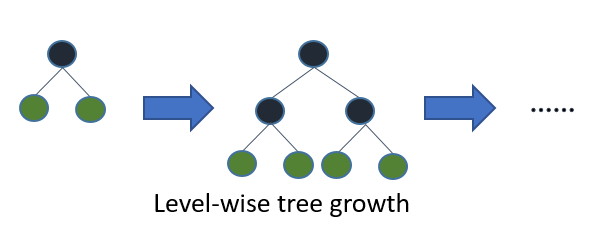
\includegraphics[width=0.65\linewidth]{figure/depthwise} 

}

\caption{Level-wise tree growth in most GBDT algorithms}\label{fig:depthwise}
\end{figure}
In contrast, the LightGBM algorithm uses a best-first approach and grows
tree leaf-wise. As a result, the tree will choose the leaf with max
delta loss to grow. According to (Microsoft Corporation, 2018), holding
the leaf fixed, leaf-wise algorithms are able to achieve better accuracy
i.e.~lower loss compared to level-wise algorithms.
\begin{figure}
\includegraphics[width=1\linewidth]{figure/leafwise} \caption{Leaf-wise tree growth in LightGBM algorithm}\label{fig:leafwise}
\end{figure}
(image source\footnote{\url{https://github.com/Microsoft/LightGBM/blob/master/docs/Features.rst\#references}})

Researcher (Shi, 2007) further explains the phenomena behind tree growth
in best-first and depth-first approach and suggests that most decision
tree learners expand nodes in depth-first order whereas best-first tree
learners expand the best node whose split achieves maximum reduction of
impurity among all the nodes available for splitting. Although the
resulting tree will be the same as a depth-wise tree, the difference is
in the order in which it grown.

One of the key advantages of using LightGBM algorithm is that it offers
good accuracy with label encoded categorical features instead of one hot
encoded features. This eventually leads to faster training time.
According to LightGBM documentation (Microsoft Corporation, 2018), the
tree built on one-hot encoded features tends to be unbalanced and needs
higher depth in order to achieve good accuracy in the case of
categorical features with high-cardinality. LightGBM implements
Exclusive Feature Bundling (EFB) technique, which is based on research
by (D. Fisher, 1958) to find the optimal split over categories and often
performs better than one-hot encoding.

One disadvantage of the leaf-wise approach is that it may cause over
fitting when data is small. To overcome this issue, LightGBM includes
the \texttt{max\_depth} parameter to control model complexity, however,
trees still grow leaf-wise even when \texttt{max\_depth} is specified
(Microsoft Corporation, 2018).

\section{Data preparation}\label{data-preparation-6}

To understand the characteristics of the top 10 most active and violent
terrorist groups, we filter the data and include all the countries that
are impacted by this groups as shown in the code chunk below:
\begin{Shaded}
\begin{Highlighting}[]
\NormalTok{df_class <-}\StringTok{ }\NormalTok{df }\OperatorTok\StringTok{ }
\StringTok{  }\KeywordTok{filter}\NormalTok{(group_name }\OperatorTok\StringTok{ }\NormalTok{top10_groups) }\OperatorTok
\StringTok{  }\KeywordTok{select}\NormalTok{(suicide_attack, year, month, day, region, country, }
\NormalTok{         provstate, city, attack_type, target_type, weapon_type, }
\NormalTok{         target_nalty, group_name, crit1_pol_eco_rel_soc, crit2_publicize, }
\NormalTok{         crit3_os_intl_hmn_law, part_of_multiple_attacks, }
\NormalTok{         individual_attack, attack_success, extended, }
\NormalTok{         intl_logistical_attack, intl_ideological_attack, }
\NormalTok{         nkill, nwound, arms_export, arms_import, population, }
\NormalTok{         gdp_per_capita, refugee_asylum, refugee_origin, }
\NormalTok{         net_migration, n_peace_keepers, conflict_index) }\OperatorTok
\StringTok{  }\KeywordTok{replace_na}\NormalTok{(}\KeywordTok{list}\NormalTok{(}\DataTypeTok{nkill =} \DecValTok{0}\NormalTok{, }\DataTypeTok{nwound =} \DecValTok{0}\NormalTok{)) }\OperatorTok
\StringTok{  }\KeywordTok{na.omit}\NormalTok{()}
\end{Highlighting}
\end{Shaded}
\section{Overview of the target
variable}\label{overview-of-the-target-variable}

For this analysis, I have selected \texttt{suicide\_attack} as a target
variable. According to GTD codebook, this variable is coded ``Yes'' in
those cases where there is evidence that the perpetrator did not intend
to escape from the attack alive.
\begin{table}[H]

\caption{\label{tab:unnamed-chunk-123}Frequency table: suicide attack variable}
\centering
\begin{tabular}[t]{lrrrr}
\toprule
level & freq & perc & cumfreq & cumperc\\
\midrule
No & 19319 & 0.887 & 19319 & 0.887\\
Yes & 2461 & 0.113 & 21780 & 1.000\\
\bottomrule
\end{tabular}
\end{table}
From the frequency table, we can see that 11.3\% of incidents were
observed as suicide attacks out of total 21,780 observations. Our
objective is to train the classifier on training data (up to 2015) and
correctly classify the instances of ``Yes'' in suicide attack variable
in test data (the year 2016).

\subsection{Dealing with class
imbalance}\label{dealing-with-class-imbalance}
\begin{figure}
\centering
\includegraphics{thesis_files/figure-latex/unnamed-chunk-124-1.pdf}
\caption{\label{fig:unnamed-chunk-124}Overview of target variable: Suicide
Attack}
\end{figure}
From the frequency table and the plot above, we can see that the target
variable has a severe class imbalance where positive cases are present
in only 11.3\% observations. For the classification modeling, the class
imbalance is a major issue and there are several techniques to deal with
it such as down sampling, up sampling, SMOTE (Synthetic Minority
Over-sampling Technique).

We use \texttt{scale\_pos\_weight} argument in the model building
process which controls the weights of the positive observations.
According to LightGBM documentation (Microsoft Corporation, 2018),
default value for \texttt{scale\_pos\_weight} is 1.0 and it represents
weight of positive class in binary classification task. We calculate
this value as a number of negative samples/number of positive samples.

\section{Feature engineering}\label{feature-engineering}

Feature engineering is a process of creating representations of data
that increase the effectiveness of a model (M. K. and K. Johnson, 2018).
This is one of the most important aspects in machine learning that
requires careful transformations and widening the feature space in order
to improve the performance of the model. During the data cleaning
process, we have already taken care of missing values and NAs. With
regard to LightGBM model, the primary requirement is to have all the
variables in numeric. As discussed earlier, LightGBM offers good
accuracy with label encoded categorical features compared to the one-hot
encoding method used in most algorithms. In this regard, we label encode
all the categorical variables and specify them as a vector in model
parameters. We also have numeric variables with extreme values such as
arms\_import, arms\_export, nkill, nwound etc. For the modeling purpose,
we use log transformation for such features. Last but not the least, we
add frequency count features to widen the feature space. Frequency count
features is a known technique in machine learning competitions to
improve the accuracy of the model. An example of the feature with
frequency is a number of attacks by the group, year and region. Use of
frequency count features adds more context to data and will be helpful
to improve the performance of the model.
\begin{Shaded}
\begin{Highlighting}[]
\CommentTok{#-------------------------------------------------------------}
\CommentTok{# Step 1: log transformation}
\CommentTok{#-------------------------------------------------------------}
\NormalTok{data <-}\StringTok{ }\NormalTok{df_class }\OperatorTok\StringTok{  }
\StringTok{  }\KeywordTok{mutate}\NormalTok{(}\DataTypeTok{nkill =} \KeywordTok{log1p}\NormalTok{(nkill }\OperatorTok{+}\StringTok{ }\FloatTok{0.01}\NormalTok{), }
         \DataTypeTok{nwound=} \KeywordTok{log1p}\NormalTok{(nwound }\OperatorTok{+}\StringTok{ }\FloatTok{0.01}\NormalTok{),}
         \DataTypeTok{arms_export =} \KeywordTok{log1p}\NormalTok{(arms_export }\OperatorTok{+}\StringTok{ }\FloatTok{0.01}\NormalTok{),}
         \DataTypeTok{arms_import =} \KeywordTok{log1p}\NormalTok{(arms_import }\OperatorTok{+}\StringTok{ }\FloatTok{0.01}\NormalTok{),}
         \DataTypeTok{population =} \KeywordTok{log1p}\NormalTok{(population }\OperatorTok{+}\StringTok{ }\FloatTok{0.01}\NormalTok{))}

\CommentTok{#--------------------------------------------------------------}
\CommentTok{# Step 2: Add frequency count features}
\CommentTok{#--------------------------------------------------------------}
\NormalTok{data <-}\StringTok{ }\KeywordTok{as.data.table}\NormalTok{(data)}
\NormalTok{data[, n_group_year}\OperatorTok{:}\ErrorTok{=}\NormalTok{.N,        by=}\KeywordTok{list}\NormalTok{(group_name, year)]}
\NormalTok{data[, n_region_year}\OperatorTok{:}\ErrorTok{=}\NormalTok{.N,       by=}\KeywordTok{list}\NormalTok{(region, year)]}
\NormalTok{data[, n_city_year}\OperatorTok{:}\ErrorTok{=}\NormalTok{.N,         by=}\KeywordTok{list}\NormalTok{(city, year)]}
\NormalTok{data[, n_attack_year}\OperatorTok{:}\ErrorTok{=}\NormalTok{.N,       by=}\KeywordTok{list}\NormalTok{(attack_type, year)]}
\NormalTok{data[, n_target_year}\OperatorTok{:}\ErrorTok{=}\NormalTok{.N,       by=}\KeywordTok{list}\NormalTok{(target_type, year)]}
\NormalTok{data[, n_weapon_year}\OperatorTok{:}\ErrorTok{=}\NormalTok{.N,       by=}\KeywordTok{list}\NormalTok{(weapon_type, year)]}
\NormalTok{data[, n_group_region_year}\OperatorTok{:}\ErrorTok{=}\NormalTok{.N, by=}\KeywordTok{list}\NormalTok{(group_name, region, year)]}
\NormalTok{data[, n_group}\OperatorTok{:}\ErrorTok{=}\NormalTok{.N,             by=}\KeywordTok{list}\NormalTok{(group_name)]}
\NormalTok{data[, n_provstate}\OperatorTok{:}\ErrorTok{=}\NormalTok{.N,         by=}\KeywordTok{list}\NormalTok{(provstate)]}
\NormalTok{data[, n_city}\OperatorTok{:}\ErrorTok{=}\NormalTok{.N,              by=}\KeywordTok{list}\NormalTok{(city)]}
\NormalTok{data <-}\StringTok{ }\KeywordTok{as.data.frame}\NormalTok{(data)}

\CommentTok{#--------------------------------------------------------------}
\CommentTok{# Step 3: label encode categorical data (lightgbm requirement)}
\CommentTok{#--------------------------------------------------------------}

\NormalTok{features=}\StringTok{ }\KeywordTok{names}\NormalTok{(data)}
\ControlFlowTok{for}\NormalTok{ (f }\ControlFlowTok{in}\NormalTok{ features) \{}
  \ControlFlowTok{if}\NormalTok{ (}\KeywordTok{class}\NormalTok{(data[[f]])}\OperatorTok{==}\StringTok{"character"}\NormalTok{) \{}
\NormalTok{    levels <-}\StringTok{ }\KeywordTok{unique}\NormalTok{(}\KeywordTok{c}\NormalTok{(data[[f]]))}
\NormalTok{    data[[f]] <-}\StringTok{ }\KeywordTok{as.integer}\NormalTok{(}\KeywordTok{factor}\NormalTok{(data[[f]], }\DataTypeTok{levels=}\NormalTok{levels))}
\NormalTok{  \}}
\NormalTok{\}}

\CommentTok{#--------------------------------------------------------------}
\CommentTok{# Step 4: Covert all the variable to numeric}
\CommentTok{#--------------------------------------------------------------}
\NormalTok{data[] <-}\StringTok{ }\KeywordTok{lapply}\NormalTok{(data, as.numeric)}
\CommentTok{#str(data)}
\end{Highlighting}
\end{Shaded}
At this point, all of our variables are numeric and there are no missing
values or NAs in this prepared data.

\section{Validation strategy}\label{validation-strategy}

In general, cross-validation is the widely used approach to estimate
performance of the model. In this approach, training data is split into
equal sized (k) folds. The model is then trained on k-1 folds and
performance is measured on the remaining fold (M. K. and K. Johnson,
2018). However, this approach is not suitable for our data. To further
explain this, the observations in our dataset are time-based so training
the model on recent years (for example 2000- 2010) and evaluating the
performance on previous years (for example 1980- 1990) would not be
meaningful. To overcome this issue, we use a time-based split to
evaluate the performance of our model. In other words, we use the
observations in the year 2016 as the test set and the remaining
observations as our training set.

This way we can be ensured that the model we have trained is capable of
classifying target variable in current context. Following is the code
used to implement validation strategy:
\begin{Shaded}
\begin{Highlighting}[]
\CommentTok{#--------------------------------------}
\CommentTok{# validation split}
\CommentTok{#--------------------------------------}
\NormalTok{train <-}\StringTok{ }\NormalTok{data }\OperatorTok\StringTok{ }\KeywordTok{filter}\NormalTok{(year }\OperatorTok{<=}\StringTok{ }\DecValTok{2015}\NormalTok{)}
\NormalTok{test  <-}\StringTok{ }\NormalTok{data }\OperatorTok\StringTok{ }\KeywordTok{filter}\NormalTok{(year }\OperatorTok{==}\StringTok{ }\DecValTok{2016}\NormalTok{)}
\end{Highlighting}
\end{Shaded}
The next stage of the process is to convert our data into lgb.Dataset
format. During this process, we create a vector containing names of all
our categorical variables and specify it while constructing lgb.Dataset
as shown in the code below:
\begin{Shaded}
\begin{Highlighting}[]
\CommentTok{#--------------------------------------}
\CommentTok{# define all categorical features}
\CommentTok{#--------------------------------------}
\NormalTok{cat_vars <-}\StringTok{ }\NormalTok{df }\OperatorTok\StringTok{ }
\StringTok{  }\KeywordTok{select}\NormalTok{(year, month, day, region, country, }
\NormalTok{         provstate, city, attack_type, target_type, weapon_type, }
\NormalTok{         target_nalty, group_name, crit1_pol_eco_rel_soc, crit2_publicize, }
\NormalTok{         crit3_os_intl_hmn_law, part_of_multiple_attacks, }
\NormalTok{         individual_attack, attack_success, extended, }
\NormalTok{         intl_logistical_attack, intl_ideological_attack, }
\NormalTok{         conflict_index) }\OperatorTok\StringTok{ }
\StringTok{  }\KeywordTok{names}\NormalTok{()}

\CommentTok{#----------------------------------------------------------------------------}
\CommentTok{# construct lgb.Dataset, and specify target variable and categorical features}
\CommentTok{#----------------------------------------------------------------------------}
\NormalTok{dtrain =}\StringTok{ }\KeywordTok{lgb.Dataset}\NormalTok{(}
  \DataTypeTok{data =} \KeywordTok{as.matrix}\NormalTok{(train[, }\KeywordTok{colnames}\NormalTok{(train) }\OperatorTok{!=}\StringTok{ "suicide_attack"}\NormalTok{]), }
  \DataTypeTok{label =}\NormalTok{ train}\OperatorTok{$}\NormalTok{suicide_attack, }
  \DataTypeTok{categorical_feature =}\NormalTok{ cat_vars}
\NormalTok{  )}

\NormalTok{dtest =}\StringTok{ }\KeywordTok{lgb.Dataset}\NormalTok{(}
  \DataTypeTok{data =} \KeywordTok{as.matrix}\NormalTok{(test[, }\KeywordTok{colnames}\NormalTok{(test) }\OperatorTok{!=}\StringTok{ "suicide_attack"}\NormalTok{]), }
  \DataTypeTok{label =}\NormalTok{ test}\OperatorTok{$}\NormalTok{suicide_attack, }
  \DataTypeTok{categorical_feature =}\NormalTok{ cat_vars}
\NormalTok{  )}
\end{Highlighting}
\end{Shaded}
Notice that we have assigned labels separately to training and test
data. To summarize the process, we will train the model on training data
(dtrain), evaluate performance on test data (dtest).

\section{Hyperparameter optimization}\label{hyperparameter-optimization}

Hyperparameter tuning is a process of finding the optimal value for the
chosen model parameter. According to (M. K. and K. Johnson, 2018),
parameter tuning is an important aspect of modeling because they control
the model complexity. And so that, it also affects any variance-base
trade-off that can be made. There are several approaches for
hyperparameter tuning such as Bayesian optimization, grid-search, and
randomized search. For this analysis, we used random grid-search
approach for hyperparameter optimization. In simple words, Randomized
grid-search means we concentrate on the hyperparameter space that looks
promising. This judgment often comes with the prior experience of
working with similar data. Several researchers (Bergstra \& Bengio,
2012; Bergstra, Bardenet, Bengio, \& Kégl, 2011) have also supported the
randomized grid-search approach and have claimed that random search is
much more efficient than any other approaches for optimizing the
parameters.

For this analysis, we choose number of leaves, max depth, bagging
fraction, feature fraction and scale positive weight which are the most
important parameters to control the complexity of the model. As shown in
the code chunk below, first we define a grid by specifying parameter and
iterate over a number of models in grids to find the optimal parameter
values.
\begin{Shaded}
\begin{Highlighting}[]
\KeywordTok{set.seed}\NormalTok{(}\DecValTok{84}\NormalTok{)}
\CommentTok{#--------------------------------------}
\CommentTok{# define grid in hyperparameter space}
\CommentTok{#--------------------------------------}
\NormalTok{grid <-}\StringTok{ }\KeywordTok{expand.grid}\NormalTok{(}
  \DataTypeTok{num_leaves        =} \KeywordTok{c}\NormalTok{(}\DecValTok{5}\NormalTok{,}\DecValTok{7}\NormalTok{,}\DecValTok{9}\NormalTok{),}
  \DataTypeTok{max_depth         =} \KeywordTok{c}\NormalTok{(}\DecValTok{4}\NormalTok{,}\DecValTok{6}\NormalTok{),}
  \DataTypeTok{bagging_fraction  =} \KeywordTok{c}\NormalTok{(}\FloatTok{0.7}\NormalTok{,}\FloatTok{0.8}\NormalTok{,}\FloatTok{0.9}\NormalTok{),}
  \DataTypeTok{feature_fraction  =} \KeywordTok{c}\NormalTok{(}\FloatTok{0.7}\NormalTok{,}\FloatTok{0.8}\NormalTok{,}\FloatTok{0.9}\NormalTok{),}
  \DataTypeTok{scale_pos_weight  =} \KeywordTok{c}\NormalTok{(}\DecValTok{4}\NormalTok{,}\DecValTok{7}\NormalTok{) }
\NormalTok{)}

\CommentTok{#--------------------------------------}
\CommentTok{# Iterate model over set grid}
\CommentTok{#--------------------------------------}
\NormalTok{model <-}\StringTok{ }\KeywordTok{list}\NormalTok{()}
\NormalTok{perf <-}\StringTok{ }\KeywordTok{numeric}\NormalTok{(}\KeywordTok{nrow}\NormalTok{(grid))}

\ControlFlowTok{for}\NormalTok{ (i }\ControlFlowTok{in} \DecValTok{1}\OperatorTok{:}\KeywordTok{nrow}\NormalTok{(grid)) \{}
  \CommentTok{# cat("Model ***", i , "*** of ", nrow(grid), "\textbackslash{}n")}
\NormalTok{  model[[i]] <-}\StringTok{ }\KeywordTok{lgb.train}\NormalTok{(}
      \KeywordTok{list}\NormalTok{(}\DataTypeTok{objective         =} \StringTok{"binary"}\NormalTok{,}
           \DataTypeTok{metric            =} \StringTok{"auc"}\NormalTok{,}
           \DataTypeTok{learning_rate     =} \FloatTok{0.01}\NormalTok{,}
           \DataTypeTok{num_leaves        =}\NormalTok{ grid[i, }\StringTok{"num_leaves"}\NormalTok{],}
           \DataTypeTok{max_depth         =}\NormalTok{ grid[i, }\StringTok{"max_depth"}\NormalTok{],}
           \DataTypeTok{bagging_fraction  =}\NormalTok{ grid[i, }\StringTok{"bagging_fraction"}\NormalTok{],}
           \DataTypeTok{feature_fraction  =}\NormalTok{ grid[i, }\StringTok{"feature_fraction"}\NormalTok{],}
           \DataTypeTok{scale_pos_weight  =}\NormalTok{ grid[i, }\StringTok{"scale_pos_weight"}\NormalTok{]),}
\NormalTok{      dtrain,}
      \DataTypeTok{valids =} \KeywordTok{list}\NormalTok{(}\DataTypeTok{validation =}\NormalTok{ dtest),}
      \DataTypeTok{nthread =} \DecValTok{4}\NormalTok{, }
      \DataTypeTok{nrounds =} \DecValTok{5}\NormalTok{,}
      \DataTypeTok{verbose=} \DecValTok{0}\NormalTok{, }
      \DataTypeTok{early_stopping_rounds =} \DecValTok{3}
\NormalTok{    )}
\NormalTok{  perf[i] <-}\StringTok{ }\KeywordTok{max}\NormalTok{(}\KeywordTok{unlist}\NormalTok{(model[[i]]}\OperatorTok{$}\NormalTok{record_evals[[}\StringTok{"validation"}\NormalTok{]][[}\StringTok{"auc"}\NormalTok{]][[}\StringTok{"eval"}\NormalTok{]]))}
  \KeywordTok{invisible}\NormalTok{(}\KeywordTok{gc}\NormalTok{()) }\CommentTok{# free up memory after each model run}
\NormalTok{\}}
\end{Highlighting}
\end{Shaded}
\begin{Shaded}
\begin{Highlighting}[]
\CommentTok{#--------------------------------------}
\CommentTok{#Extract results}
\CommentTok{#--------------------------------------}
\KeywordTok{cat}\NormalTok{(}\StringTok{"Model "}\NormalTok{, }\KeywordTok{which.max}\NormalTok{(perf), }\StringTok{" is with max AUC: "}\NormalTok{, }\KeywordTok{max}\NormalTok{(perf), }\DataTypeTok{sep =} \StringTok{""}\NormalTok{,}\StringTok{"}\CharTok{\textbackslash{}n}\StringTok{"}\NormalTok{)}
\end{Highlighting}
\end{Shaded}
\begin{verbatim}
Model 42 is with max AUC: 0.9538
\end{verbatim}
\begin{Shaded}
\begin{Highlighting}[]
\NormalTok{best_params =}\StringTok{ }\NormalTok{grid[}\KeywordTok{which.max}\NormalTok{(perf), ]}
\end{Highlighting}
\end{Shaded}
\begin{table}[H]

\caption{\label{tab:unnamed-chunk-130}Hyperparameter tuning result}
\centering
\fontsize{12}{14}\selectfont
\begin{tabular}[t]{lrrrrr}
\toprule
  & num\_leaves & max\_depth & bagging\_fraction & feature\_fraction & scale\_pos\_weight\\
\midrule
42 & 9 & 6 & 0.7 & 0.9 & 4\\
\bottomrule
\end{tabular}
\end{table}
From the hyperparameter tuning, we have extracted the optimized values
based on AUC. Next, we use these parameters in the model building
process.

\section{Modelling}\label{modelling-3}
\begin{Shaded}
\begin{Highlighting}[]
\CommentTok{# assign params from hyperparameter tuning result}
\NormalTok{params <-}\StringTok{ }\KeywordTok{list}\NormalTok{(}\DataTypeTok{objective =} \StringTok{"binary"}\NormalTok{, }
               \DataTypeTok{metric =} \StringTok{"auc"}\NormalTok{, }
               \DataTypeTok{num_leaves =}\NormalTok{ best_params}\OperatorTok{$}\NormalTok{num_leaves,}
               \DataTypeTok{max_depth =}\NormalTok{ best_params}\OperatorTok{$}\NormalTok{max_depth,}
               \DataTypeTok{bagging_fraction =}\NormalTok{ best_params}\OperatorTok{$}\NormalTok{bagging_fraction,}
               \DataTypeTok{feature_fraction =}\NormalTok{ best_params}\OperatorTok{$}\NormalTok{feature_fraction,}
               \DataTypeTok{scale_pos_weight=}\NormalTok{ best_params}\OperatorTok{$}\NormalTok{scale_pos_weight,}
               \DataTypeTok{bagging_freq =} \DecValTok{1}\NormalTok{,}
               \DataTypeTok{learning_rate =} \FloatTok{0.01}\NormalTok{)}

\NormalTok{model <-}\StringTok{ }\KeywordTok{lgb.train}\NormalTok{(params, }
\NormalTok{                   dtrain, }
                   \DataTypeTok{valids =} \KeywordTok{list}\NormalTok{(}\DataTypeTok{validation =}\NormalTok{ dtest), }
                   \DataTypeTok{nrounds =} \DecValTok{1000}\NormalTok{, }
                   \DataTypeTok{early_stopping_rounds =} \DecValTok{50}\NormalTok{,}
                   \DataTypeTok{eval_freq =} \DecValTok{100}\NormalTok{)}
\end{Highlighting}
\end{Shaded}
\begin{verbatim}
[1]:    validation's auc:0.937756 
[101]:  validation's auc:0.961098 
[201]:  validation's auc:0.962072 
[301]:  validation's auc:0.963493 
\end{verbatim}
\subsection{Model evaluation}\label{model-evaluation}

In order to evaluate the performance of our model on test data, we have
used AUC metric which is commonly used in binary classification problem.
From the trained model, we extract AUC score on test data from the best
iteration with the code as shown below:
\begin{Shaded}
\begin{Highlighting}[]
\KeywordTok{cat}\NormalTok{(}\StringTok{"Best iteration: "}\NormalTok{, model}\OperatorTok{$}\NormalTok{best_iter, }\StringTok{"}\CharTok{\textbackslash{}n}\StringTok{"}\NormalTok{)}
\end{Highlighting}
\end{Shaded}
\begin{verbatim}
Best iteration:  288 
\end{verbatim}
\begin{Shaded}
\begin{Highlighting}[]
\KeywordTok{cat}\NormalTok{(}\StringTok{"Validation AUC @ best iter: "}\NormalTok{, }
    \KeywordTok{max}\NormalTok{(}\KeywordTok{unlist}\NormalTok{(model}\OperatorTok{$}\NormalTok{record_evals[[}\StringTok{"validation"}\NormalTok{]][[}\StringTok{"auc"}\NormalTok{]][[}\StringTok{"eval"}\NormalTok{]])), }\StringTok{"}\CharTok{\textbackslash{}n}\StringTok{"}\NormalTok{)}
\end{Highlighting}
\end{Shaded}
\begin{verbatim}
Validation AUC @ best iter:  0.9636 
\end{verbatim}
To deal with overfitting, we have specified early stopping criteria
which stops the model training if no improvement is observed within
specified rounds. At the best iteration, our model achieves 96.36\%
accuracy on validation data. To further investigate the error rate, we
use the confusion matrix.

\subsection{Confusion Matrix}\label{confusion-matrix}

A confusion matrix is an another way to evaluate performance of binary
classification model.
\begin{Shaded}
\begin{Highlighting}[]
\CommentTok{# get predictions on validation data}
\NormalTok{test_matrix <-}\StringTok{ }\KeywordTok{as.matrix}\NormalTok{(test[, }\KeywordTok{colnames}\NormalTok{(test) }\OperatorTok{!=}\StringTok{ "suicide_attack"}\NormalTok{])}
\NormalTok{test_preds =}\StringTok{ }\KeywordTok{predict}\NormalTok{(model, }\DataTypeTok{data =}\NormalTok{ test_matrix, }\DataTypeTok{n =}\NormalTok{ model}\OperatorTok{$}\NormalTok{best_iter)}

\KeywordTok{confusionMatrix}\NormalTok{(}
  \DataTypeTok{data =} \KeywordTok{as.factor}\NormalTok{(}\KeywordTok{ifelse}\NormalTok{(test_preds }\OperatorTok{>}\StringTok{ }\FloatTok{0.5}\NormalTok{, }\DecValTok{1}\NormalTok{, }\DecValTok{0}\NormalTok{)), }
  \DataTypeTok{reference =} \KeywordTok{as.factor}\NormalTok{(test}\OperatorTok{$}\NormalTok{suicide_attack)}
\NormalTok{  )}
\end{Highlighting}
\end{Shaded}
\begin{verbatim}
Confusion Matrix and Statistics

          Reference
Prediction    0    1
         0 3339   91
         1  249  582
                                             
               Accuracy : 0.92               
                 95% CI : (0.912, 0.928)     
    No Information Rate : 0.842              
    P-Value [Acc > NIR] : <0.0000000000000002
                                             
                  Kappa : 0.726              
 Mcnemar's Test P-Value : <0.0000000000000002
                                             
            Sensitivity : 0.931              
            Specificity : 0.865              
         Pos Pred Value : 0.973              
         Neg Pred Value : 0.700              
             Prevalence : 0.842              
         Detection Rate : 0.784              
   Detection Prevalence : 0.805              
      Balanced Accuracy : 0.898              
                                             
       'Positive' Class : 0                  
                                             
\end{verbatim}
The accuracy of 0.92 indicates that our model is 92\% accurate. Out of
all the metrics, the one we are most interested in is specificity. We
want our classifier to predict the ``Yes''/ ``1'' instances of suicide
attack with higher accuracy. From the contingency table, we can see that
our model has correctly predicted 582 out of 673 instances of ``1''/
``Yes'' in suicide attacks and achieves an accuracy of 86.5\%.

\subsection{Feature importance}\label{feature-importance}
\begin{Shaded}
\begin{Highlighting}[]
\CommentTok{# get feature importance}
\NormalTok{fi =}\StringTok{ }\KeywordTok{lgb.importance}\NormalTok{(model, }\DataTypeTok{percentage =} \OtherTok{TRUE}\NormalTok{)}
\end{Highlighting}
\end{Shaded}
\begin{table}[H]

\caption{\label{tab:unnamed-chunk-135}Feature importance matrix (Top 15)}
\centering
\fontsize{13}{15}\selectfont
\begin{tabular}[t]{lrrr}
\toprule
Feature & Gain & Cover & Frequency\\
\midrule
weapon\_type & 0.4447 & 0.2088 & 0.0773\\
nkill & 0.1883 & 0.1298 & 0.1389\\
provstate & 0.1285 & 0.2174 & 0.2370\\
attack\_type & 0.0781 & 0.1080 & 0.0616\\
target\_type & 0.0353 & 0.0618 & 0.0964\\
\addlinespace
nwound & 0.0291 & 0.0591 & 0.0820\\
attack\_success & 0.0229 & 0.0244 & 0.0464\\
city & 0.0221 & 0.0979 & 0.0543\\
day & 0.0110 & 0.0279 & 0.0699\\
n\_attack\_year & 0.0069 & 0.0095 & 0.0195\\
\addlinespace
group\_name & 0.0067 & 0.0081 & 0.0165\\
n\_peace\_keepers & 0.0052 & 0.0049 & 0.0143\\
refugee\_origin & 0.0048 & 0.0048 & 0.0130\\
target\_nalty & 0.0033 & 0.0121 & 0.0156\\
n\_city\_year & 0.0018 & 0.0019 & 0.0043\\
\bottomrule
\end{tabular}
\end{table}
Gain is the most important measure for predictions and represents
feature contribution to the model. This is calculated by comparing the
contribution of each feature for each tree in the model. The Cover
metric indicates a number of observations related to the particular
feature. The Frequency measure is the percentage representing the
relative number of times a particular feature occurs in the trees of the
model. In simple words, it tells us how often the feature is used in the
model (T. Chen, Tong, Benesty, \& Tang, 2018; Pandya, 2018).

From the feature importance matrix, we can see that type of weapon
contributes the most in terms of gain followed by number of people
killed, province state, type of attack and type of target. In order to
allow the model to decide whether an attack will be a suicide attack or
not, these features are the most important compared to others.

\section{Model interpretation}\label{model-interpretation}

To further analyze the reasoning behind the model's decision-making
process, we randomly select one observation from test data and compare
it with the predicted value based on features contribution. With the
code chunk as shown below, we have extracted the predicted value from
our trained model for the second observation in the test data.
\begin{Shaded}
\begin{Highlighting}[]
\KeywordTok{cat}\NormalTok{(}\KeywordTok{paste}\NormalTok{(}\StringTok{"predicted value from model: "}\NormalTok{, test_preds[[}\DecValTok{2}\NormalTok{]]))}
\end{Highlighting}
\end{Shaded}
\begin{verbatim}
predicted value from model:  0.854690873381908
\end{verbatim}
The predicted value is 0.85 (i.e. \textgreater{} 0.5) which means our
model indicates that the incident likely to be a suicide attack (i.e.
``Yes'' instance in suicide attack variable). Next, we use
\texttt{lgb.interpret} function to compute feature contribution
components of raw score prediction for this observation.
\begin{Shaded}
\begin{Highlighting}[]
\CommentTok{#extract interpretation for 2nd observation in (transformed) test data}
\NormalTok{test_matrix <-}\StringTok{ }\KeywordTok{as.matrix}\NormalTok{(test[, }\KeywordTok{colnames}\NormalTok{(test)])}
\NormalTok{tree_interpretation <-}\StringTok{ }\KeywordTok{lgb.interprete}\NormalTok{(model, }\DataTypeTok{data =}\NormalTok{ test_matrix, }\DataTypeTok{idxset =} \DecValTok{2}\NormalTok{)}
\end{Highlighting}
\end{Shaded}
\begin{figure}
\includegraphics[width=1\linewidth]{thesis_files/figure-latex/unnamed-chunk-138-1} \caption{Model interpretation for 2nd observation}\label{fig:unnamed-chunk-138}
\end{figure}
In the plot above, ten most important features (with higher
contribution) are shown on the Y axis and their contribution value is on
the X-axis. The negative value indicates contradiction and a positive
value represents support. Our trained model has taken the decision to
predict 0.85 for the second observation based on the contribution level
of the above-mentioned features. Although nkill and weapon\_type
variables are one of most important features based on gain however their
contribution toward prediction is negative. On the other hand, province,
city, attack type and attack success features have a positive value
which indicates support.

In our model, we have transformed the data to numeric. However, we can
extract the raw test data (before transformation) and specific columns
to compare the actual values with feature contribution plot above.
\begin{Shaded}
\begin{Highlighting}[]
\CommentTok{# extract raw test data}
\NormalTok{tmp_test <-}\StringTok{ }\NormalTok{df_class }\OperatorTok\StringTok{ }
\StringTok{  }\KeywordTok{filter}\NormalTok{(year }\OperatorTok{==}\StringTok{ }\DecValTok{2016}\NormalTok{) }\OperatorTok
\StringTok{  }\KeywordTok{select}\NormalTok{(suicide_attack, nkill, provstate, weapon_type, }
\NormalTok{         attack_type, city, attack_success, target_type, }
\NormalTok{         refugee_origin, n_peace_keepers)}

\CommentTok{# Extract second observation}
\NormalTok{tmp_test <-}\StringTok{ }\KeywordTok{as.data.frame}\NormalTok{(}\KeywordTok{t}\NormalTok{(tmp_test[}\DecValTok{2}\NormalTok{, ]))}

\CommentTok{# display result}
\NormalTok{knitr}\OperatorTok{::}\KeywordTok{kable}\NormalTok{(tmp_test, }\DataTypeTok{booktabs=} \OtherTok{TRUE}\NormalTok{,}
             \DataTypeTok{caption =} \StringTok{"Actual values in 2nd observation in test set"}\NormalTok{) }\OperatorTok
\StringTok{  }\KeywordTok{kable_styling}\NormalTok{(}\DataTypeTok{latex_options =} \StringTok{"HOLD_position"}\NormalTok{, }\DataTypeTok{font_size =} \DecValTok{12}\NormalTok{, }\DataTypeTok{full_width =}\NormalTok{ F)}
\end{Highlighting}
\end{Shaded}
\begin{table}[H]

\caption{\label{tab:unnamed-chunk-139}Actual values in 2nd observation in test set}
\centering
\fontsize{12}{14}\selectfont
\begin{tabular}[t]{ll}
\toprule
  & 2\\
\midrule
suicide\_attack & 1\\
nkill & 3\\
provstate & Kabul\\
weapon\_type & Explosives/Bombs/Dynamite\\
attack\_type & Bombing/Explosion\\
\addlinespace
city & Kabul\\
attack\_success & 1\\
target\_type & Business\\
refugee\_origin & 2501410\\
n\_peace\_keepers & 14\\
\bottomrule
\end{tabular}
\end{table}
The predicted value from our model for the second observation is 0.85
and comparing it with actual value suggests that the incident was, in
fact, a suicide attack as shown in the table above where the value is
``1'' in suicide attack variable. For this specific observation, our
model suggests that Kabul as a city and provstate, Bombing/Explosion as
attack type and attack being successful contributes positively toward
prediction. In contrast, 3 fatalities, business as a target type and
explosives as a weapon type contributes negatively to the prediction.
Our trained model has correctly predicted 582 out of 673 instances of
``1''/ ``Yes'' in suicide attacks and achieves an accuracy of 86.5\%
with this decision making process.

\chapter{Discussion and Conclusion}\label{conclusion}

This thesis research set out to gain a better understanding about threat
level and characteristics of most lethal terrorist groups that are
currently active and responsible for the sudden increase in violent
terrorism around the world in present years. The outcome of this study
provides descriptive and predictive analysis and serves as an actionable
intelligence toward counterterrorism support.

We analyzed the real-world dataset of global terrorist incidents and
during exploratory data analysis, we found a nearly same trend in the
increased number of attacks from the year 2010 in the Middle East \&
North Africa, South Asia, Sub-Saharan Africa and Southeast Asia region.
Ensuring the implications in the present context, we determined the top
10 most active and violent terrorist groups and examined their
characteristics based on past incidents. We found that most of these
groups (6 out of 10) were formed after 2006 only. Upon analyzing their
attack tactics, we found that bombing/explosions account the most in
terms of attack type as well as the significantly increased use of
explosives. For example, more than 2300 incidents each year (from 2014
to 2016) involved the use of explosives. Up to a certain extent, this
indicates an easy access to sophisticated weapons, explosive devices,
and DIY material online. The double-edged sword of information age
further fuels the upward trend in use of explosives. For example, ISIL
which is one of the deadliest groups in our top ten list makes use of
social media such as Twitter and YouTube to spread the ideology through
propaganda videos and materials. Although algorithms can detect and
remove such materials from the web but the burning question we ask is
how fast? An easy access to such materials on the web, specifically
involving tutorial on making bombs and DIY kits makes terrorism the most
preferred means of waging war in present years. It is needless to
mention that increased radicalized attacks around the world are an
indication that terrorism transitioning from a place to an idea.

Within \protect\hyperlink{impact-analysis}{Impact Analysis} chapter, we
examined the threat level from these groups and identified major and
minor epicenters geographically based on a number of attacks, and
corresponding cumulative fatalities and injuries. Based on findings, we
conclude that 7 out of 10 groups (i.e.~ISIL and Taliban) are operating
decentralized and have their activity/ spread across many cities with
the varying threat level. This strategy makes them difficult to chase in
terms of combat, however, remaining three groups (Al-Nusrah Front,
Houthi Extremists and Donetsk People's Republic) have major epicenters
based on threat level in just a few cities. To understand the political
intentions behind attacks from all 10 groups, we analyzed the pattern by
targets and found that 46.7\% attacks were targeted at military and
police followed by 27.3\% attacks on civilians. To investigate
similarity and differences between each of these groups with respect to
fatalities, we performed statistical analysis. Results from our
experiment suggest non-significantly different means in Boko Haram - Al
Nusrah, Al Qaida in Arabian Peninsula (AQAP)- Al Shabaab, Houthi
Extremist- PKK etc. Similarly, pairs of ISIL with all the remaining
groups, Taliban - Al Nusrah, PKK - Boko Haram etc. suggests
significantly different means with respect to fatalities.

One of the key findings from this research is pattern discovery within
the individual group to describe how things are related and
interconnected with each other. Using Apriori algorithm, an unsupervised
machine learning technique, this research discovers 20 frequent patterns
(association rules) in ISIL group, 61 patterns in Taliban group and 27
patterns in Boko Haram group with confidence value greater than 0.5. The
confidence of 0.5 means the rule is correct at least 50\% of the time.
Results from our experiment suggest that use of a chemical weapon (with
unarmed assault or with bombings/explosion) from ISIL (0.9 confidence)
and Taliban (0.88 confidence) has maximum likelihood among all the
discovered patterns. Some other interesting patterns we find is that
ISIL is more likely to attack other terrorists/ informants for terrorist
groups (non-state militia) with bombing/explosion while having resulting
fatalities between 6 to 10 whereas Boko Haram is more likely to attack
civilians with explosives, without suicide attack and while having
resulting fatalities more than 50 in a single incident. In case of
Taliban, we find that police is the likely target with an incident
involving the use of firearms and resulting fatalities between 11 to 50.

This research also contributes positively to existing literature in
terrorism research within supervised machine learning context. Previous
research in time-series forecasting is limited to country and year level
resolution. In this research, we have extended the previous study with
seasonality components and have achieved resolution at a monthly
frequency. Using Auto Arima, Neural Network, TBATS and ETS model, we
have forecasted a number of attacks in Afghanistan and SAHEL region, and
number of fatalities in Iraq. We have evaluated and compared the
performance of each model on hold out set using several metrics before
making an actual forecast. Our findings suggest that the model that
works best in one time-series data may not be the best in another
time-series data. We also illustrated the importance of using ensemble
method and evaluated predicted vs actual values using Theil's U
statistic. Our experiment on three different time-series data using an
ensemble approach shows significant improvement in forecasting accuracy
when compared to best single models.

Similarly, in the classification task, previous research lacks the use
of algorithms that are recently developed and that (practically) out
perform traditional algorithms such as random forests, logistic
regression or J48. We have extended the previous research in binary
classification context involving severe class imbalance and have made
use of a cutting-edge LightGBM algorithm to predict the class
probability of an attack involving a suicide attempt. We have also
proposed an alternate strategy for model evaluation and have described
the reasons why standard validation techniques such as cross-validation
would be a bad choice for this data. Using the explainer object, we have
also investigated the decision-making process for each prediction from
our trained model. Our model achieves 96\% accuracy in terms of AUC
metric and 86.5\% accuracy in terms of specificity by correctly
classifying 582 out of 673 instances of actual suicide attacks in
Afghanistan.

\section{Research limitations and future
work}\label{research-limitations-and-future-work}

This research uses the most recently published (June 2017 release) data
of the Global Terrorism Database which includes incidents up to the year
2016 only. Future work in this direction can be carried out depending on
availability of new data. Within the pattern discovery part, this
research is focused on the top ten groups. Possible future work could be
to discover patterns by geographical location (i.e.~city/ state) or by
years to add more contexts in pattern discovery. Within time-series
forecasting part, possible future work can be carried out by adding some
other diverse models and using different techniques within ensemble
approach such as weighted average to evaluate improvement in accuracy.

Although machine learning works the best on structured data however
recent developments in deep learning framework for tabular data is
drawing a lot of attention nowadays. Possible Future work to investigate
threat level and characteristics of most violent terrorist groups and
corresponding forecasting can be carried out using \emph{embeddings for
the categorical variables} approach in deep learning.

\appendix

\hypertarget{appendix-i}{\chapter{Appendix I}\label{appendix-i}}

\section{Initial data preparation
script}\label{initial-data-preparation-script}
\begin{Shaded}
\begin{Highlighting}[]
\ControlFlowTok{if}\NormalTok{ (}\OperatorTok{!}\KeywordTok{require}\NormalTok{(}\StringTok{"pacman"}\NormalTok{)) }\KeywordTok{install.packages}\NormalTok{(}\StringTok{"pacman"}\NormalTok{)}
\NormalTok{pacman}\OperatorTok{::}\KeywordTok{p_load}\NormalTok{(knitr, pryr, openxlsx, tidyverse, }
\NormalTok{               data.table, DT, DescTools, RCurl, countrycode)}
\KeywordTok{options}\NormalTok{(}\DataTypeTok{warn =} \OperatorTok{-}\DecValTok{1}\NormalTok{, }\DataTypeTok{digits =} \DecValTok{4}\NormalTok{, }\DataTypeTok{scipen =} \DecValTok{999}\NormalTok{)}
\CommentTok{#------------------------------------------------------------}
\CommentTok{#External data (country geocodes to replace missing lat lons)}
\CommentTok{#------------------------------------------------------------}
\NormalTok{geocodes <-}\KeywordTok{fread}\NormalTok{(}\StringTok{"https://github.com/oughton/geocode/raw/master/example/result.csv"}\NormalTok{)}\OperatorTok
\StringTok{  }\KeywordTok{select}\NormalTok{(}\DataTypeTok{country =}\NormalTok{ V1, }\DataTypeTok{country_latitude =}\NormalTok{ V2, }\DataTypeTok{country_longitude =}\NormalTok{ V3) }\OperatorTok
\StringTok{  }\KeywordTok{mutate}\NormalTok{(}\DataTypeTok{ISO =} \KeywordTok{countrycode}\NormalTok{(country, }\StringTok{'country.name'}\NormalTok{, }\StringTok{'iso3c'}\NormalTok{)) }\OperatorTok
\StringTok{  }\KeywordTok{filter}\NormalTok{(}\OperatorTok{!}\KeywordTok{is.na}\NormalTok{(ISO)) }\OperatorTok
\StringTok{  }\KeywordTok{select}\NormalTok{(ISO, country_latitude, country_longitude)}

\KeywordTok{saveRDS}\NormalTok{(geocodes, }\StringTok{"country_geocodes.rds"}\NormalTok{)  }
\NormalTok{country_geocodes <-}\StringTok{ }\KeywordTok{readRDS}\NormalTok{(}\StringTok{"country_geocodes.rds"}\NormalTok{)}

\CommentTok{#---------------------------------------}
\CommentTok{#data preparation (GTD)}
\CommentTok{#---------------------------------------}
\NormalTok{tmp <-}\StringTok{ }\KeywordTok{read.xlsx}\NormalTok{(}\StringTok{"data/data_preparation/globalterrorismdb_0617dist.xlsx"}\NormalTok{, }
                 \DataTypeTok{sheet =} \DecValTok{1}\NormalTok{, }\DataTypeTok{colNames =} \OtherTok{TRUE}\NormalTok{) }\OperatorTok\StringTok{ }
\StringTok{  }\KeywordTok{select}\NormalTok{(eventid, }
         \DataTypeTok{year =}\NormalTok{ iyear, }
         \DataTypeTok{month =}\NormalTok{ imonth, }
         \DataTypeTok{day =}\NormalTok{ iday, }
         \DataTypeTok{country =}\NormalTok{ country_txt, }
         \DataTypeTok{region =}\NormalTok{ region_txt, }
\NormalTok{         provstate, }
\NormalTok{         city, }
\NormalTok{         latitude, }\CommentTok{# 2.7% NAs will be replaced with country level geocodes}
\NormalTok{         longitude,}
         \DataTypeTok{attack_type =}\NormalTok{ attacktype1_txt, }
         \DataTypeTok{weapon_type =}\NormalTok{ weaptype1_txt, }
         \DataTypeTok{target_type =}\NormalTok{ targtype1_txt, }
         \DataTypeTok{target_nalty=}\NormalTok{ natlty1_txt, }
         \DataTypeTok{group_name  =}\NormalTok{ gname, }
\NormalTok{         nkill,   }\CommentTok{# 5% NAs}
\NormalTok{         nwound,  }\CommentTok{# 9% NAs}
\NormalTok{         extended, }
         \DataTypeTok{crit1_pol_eco_rel_soc =}\NormalTok{ crit1, }
         \DataTypeTok{crit2_publicize =}\NormalTok{ crit2, }
         \DataTypeTok{crit3_os_intl_hmn_law =}\NormalTok{ crit3, }
         \DataTypeTok{part_of_multiple_attacks =}\NormalTok{ multiple, }
         \DataTypeTok{attack_success =}\NormalTok{ success, }
         \DataTypeTok{suicide_attack =}\NormalTok{ suicide, }
         \DataTypeTok{individual_attack =}\NormalTok{ individual,}
         \DataTypeTok{intl_logistical_attack =}\NormalTok{ INT_LOG, }
         \DataTypeTok{intl_ideological_attack =}\NormalTok{ INT_IDEO }
\NormalTok{         ) }\OperatorTok
\StringTok{  }\KeywordTok{replace_na}\NormalTok{(}\KeywordTok{list}\NormalTok{(}\DataTypeTok{provstate =} \StringTok{"unknown"}\NormalTok{,       }\CommentTok{# replace nas with unknown}
                  \DataTypeTok{city =}  \StringTok{"unknown"}\NormalTok{,}
                  \DataTypeTok{target_nalty =} \StringTok{"unknown"}\NormalTok{)) }\OperatorTok
\StringTok{  }\KeywordTok{mutate}\NormalTok{(}\DataTypeTok{ISO =} \KeywordTok{countrycode}\NormalTok{(country, }\StringTok{'country.name'}\NormalTok{, }\StringTok{'iso3c'}\NormalTok{), }\CommentTok{#standardize country name}
         \DataTypeTok{month =} \KeywordTok{if_else}\NormalTok{(month }\OperatorTok{==}\StringTok{ }\DecValTok{0}\NormalTok{, }\DecValTok{1}\NormalTok{, month),}\CommentTok{#replace unknown month to 1 in 20 occurences }
         \DataTypeTok{day =} \KeywordTok{if_else}\NormalTok{(day }\OperatorTok{==}\StringTok{ }\DecValTok{0}\NormalTok{, }\DecValTok{1}\NormalTok{, day), }\CommentTok{#replace unknown day to 1 in 891 occurences}
         \DataTypeTok{date =} \KeywordTok{paste}\NormalTok{(year, month, day, }\DataTypeTok{sep=}\StringTok{"-"}\NormalTok{),}
         \DataTypeTok{date =} \KeywordTok{as.Date}\NormalTok{(date, }\DataTypeTok{format =} \StringTok{"%Y-%m-%d"}\NormalTok{),}
         \DataTypeTok{weapon_type =} \KeywordTok{if_else}\NormalTok{(}
\NormalTok{           weapon_type }\OperatorTok{==}\StringTok{ "Vehicle (not to include vehicle-borne}
\StringTok{                           explosives, i.e., car or truck bombs)"}\NormalTok{, }
                          \StringTok{"Vehicle"}\NormalTok{, weapon_type)) }\OperatorTok\StringTok{ }\CommentTok{# shorten lengthy name}
\StringTok{  }\KeywordTok{left_join}\NormalTok{(country_geocodes) }\OperatorTok\StringTok{ }
\StringTok{  }\KeywordTok{mutate}\NormalTok{(}\DataTypeTok{latitude =} \KeywordTok{ifelse}\NormalTok{(}\KeywordTok{is.na}\NormalTok{(latitude), country_latitude, }
\NormalTok{                           latitude), }\CommentTok{# replace missing lat lons with country lat lons}
         \DataTypeTok{longitude =} \KeywordTok{ifelse}\NormalTok{(}\KeywordTok{is.na}\NormalTok{(longitude), country_longitude, longitude)) }\OperatorTok
\StringTok{  }\KeywordTok{select}\NormalTok{(}\OperatorTok{-}\KeywordTok{c}\NormalTok{(country_latitude, country_longitude)) }\OperatorTok
\StringTok{  }\CommentTok{# replace missing lat lons in remaining (~14) disputed/dissolved countries }
\StringTok{  }\CommentTok{# with country level lat long from prev obs}
\StringTok{  }\KeywordTok{mutate}\NormalTok{(}
    \DataTypeTok{latitude =} \KeywordTok{if_else}\NormalTok{(}\KeywordTok{is.na}\NormalTok{(latitude) }\OperatorTok{&}\StringTok{ }\NormalTok{country }\OperatorTok{==}\StringTok{ }
\StringTok{                          "People's Republic of the Congo"}\NormalTok{, }\OperatorTok{-}\FloatTok{0.2}\NormalTok{, latitude),}
     \DataTypeTok{longitude =} \KeywordTok{if_else}\NormalTok{(}\KeywordTok{is.na}\NormalTok{(longitude) }\OperatorTok{&}\StringTok{ }\NormalTok{country }\OperatorTok{==}\StringTok{ }
\StringTok{                           "People's Republic of the Congo"}\NormalTok{, }\FloatTok{15.8}\NormalTok{, longitude),}
     \DataTypeTok{latitude =} \KeywordTok{if_else}\NormalTok{(}\KeywordTok{is.na}\NormalTok{(latitude) }\OperatorTok{&}\StringTok{ }\NormalTok{country }\OperatorTok{==}\StringTok{ }
\StringTok{                          "Democratic Republic of the Congo"}\NormalTok{, }\OperatorTok{-}\FloatTok{4.0}\NormalTok{, latitude),}
     \DataTypeTok{longitude =} \KeywordTok{if_else}\NormalTok{(}\KeywordTok{is.na}\NormalTok{(longitude) }\OperatorTok{&}\StringTok{ }\NormalTok{country }\OperatorTok{==}\StringTok{ }
\StringTok{                           "Democratic Republic of the Congo"}\NormalTok{, }\FloatTok{21.7}\NormalTok{, longitude),}
     \DataTypeTok{latitude =} \KeywordTok{if_else}\NormalTok{(}\KeywordTok{is.na}\NormalTok{(latitude) }\OperatorTok{&}\StringTok{ }\NormalTok{country }\OperatorTok{==}\StringTok{ }
\StringTok{                          "North Yemen"}\NormalTok{, }\FloatTok{15.5}\NormalTok{, latitude),}
     \DataTypeTok{longitude =} \KeywordTok{if_else}\NormalTok{(}\KeywordTok{is.na}\NormalTok{(longitude) }\OperatorTok{&}\StringTok{ }\NormalTok{country }\OperatorTok{==}\StringTok{ }
\StringTok{                           "North Yemen"}\NormalTok{, }\FloatTok{48.5}\NormalTok{, longitude),}
     \DataTypeTok{latitude =} \KeywordTok{if_else}\NormalTok{(}\KeywordTok{is.na}\NormalTok{(latitude) }\OperatorTok{&}\StringTok{ }\NormalTok{country }\OperatorTok{==}\StringTok{ }
\StringTok{                          "South Yemen"}\NormalTok{, }\FloatTok{12.8}\NormalTok{, latitude),}
     \DataTypeTok{longitude =} \KeywordTok{if_else}\NormalTok{(}\KeywordTok{is.na}\NormalTok{(longitude) }\OperatorTok{&}\StringTok{ }\NormalTok{country }\OperatorTok{==}\StringTok{ }
\StringTok{                           "South Yemen"}\NormalTok{, }\FloatTok{45.0}\NormalTok{, longitude),}
     \DataTypeTok{latitude =} \KeywordTok{if_else}\NormalTok{(}\KeywordTok{is.na}\NormalTok{(latitude) }\OperatorTok{&}\StringTok{ }\NormalTok{country }\OperatorTok{==}\StringTok{ }
\StringTok{                          "Western Sahara"}\NormalTok{, }\FloatTok{27.4}\NormalTok{, latitude),}
     \DataTypeTok{longitude =} \KeywordTok{if_else}\NormalTok{(}\KeywordTok{is.na}\NormalTok{(longitude) }\OperatorTok{&}\StringTok{ }\NormalTok{country }\OperatorTok{==}\StringTok{ }
\StringTok{                           "Western Sahara"}\NormalTok{, }\OperatorTok{-}\FloatTok{9.0}\NormalTok{, longitude),}
     \DataTypeTok{latitude =} \KeywordTok{if_else}\NormalTok{(}\KeywordTok{is.na}\NormalTok{(latitude) }\OperatorTok{&}\StringTok{ }\NormalTok{country }\OperatorTok{==}\StringTok{ }
\StringTok{                          "Guadeloupe"}\NormalTok{, }\FloatTok{16.2}\NormalTok{, latitude),}
     \DataTypeTok{longitude =} \KeywordTok{if_else}\NormalTok{(}\KeywordTok{is.na}\NormalTok{(longitude) }\OperatorTok{&}\StringTok{ }\NormalTok{country }\OperatorTok{==}\StringTok{ }
\StringTok{                           "Guadeloupe"}\NormalTok{, }\OperatorTok{-}\FloatTok{61.5}\NormalTok{, longitude),}
     \DataTypeTok{latitude =} \KeywordTok{if_else}\NormalTok{(}\KeywordTok{is.na}\NormalTok{(latitude) }\OperatorTok{&}\StringTok{ }\NormalTok{country }\OperatorTok{==}\StringTok{ }
\StringTok{                          "New Caledonia"}\NormalTok{, }\OperatorTok{-}\FloatTok{20.9}\NormalTok{, latitude),}
     \DataTypeTok{longitude =} \KeywordTok{if_else}\NormalTok{(}\KeywordTok{is.na}\NormalTok{(longitude) }\OperatorTok{&}\StringTok{ }\NormalTok{country }\OperatorTok{==}\StringTok{ }
\StringTok{                           "New Caledonia"}\NormalTok{, }\FloatTok{165.6}\NormalTok{, longitude),}
     \DataTypeTok{latitude =} \KeywordTok{if_else}\NormalTok{(}\KeywordTok{is.na}\NormalTok{(latitude) }\OperatorTok{&}\StringTok{ }\NormalTok{country }\OperatorTok{==}\StringTok{ "Martinique"}\NormalTok{, }\FloatTok{14.6}\NormalTok{, latitude),}
     \DataTypeTok{longitude =} \KeywordTok{if_else}\NormalTok{(}\KeywordTok{is.na}\NormalTok{(longitude) }\OperatorTok{&}\StringTok{ }\NormalTok{country }\OperatorTok{==}\StringTok{ "Martinique"}\NormalTok{, }\OperatorTok{-}\FloatTok{61.0}\NormalTok{, longitude),}
     \DataTypeTok{latitude =} \KeywordTok{if_else}\NormalTok{(}\KeywordTok{is.na}\NormalTok{(latitude) }\OperatorTok{&}\StringTok{ }\NormalTok{country }\OperatorTok{==}\StringTok{ "Zaire"}\NormalTok{, }\OperatorTok{-}\FloatTok{2.5}\NormalTok{, latitude),}
     \DataTypeTok{longitude =} \KeywordTok{if_else}\NormalTok{(}\KeywordTok{is.na}\NormalTok{(longitude) }\OperatorTok{&}\StringTok{ }\NormalTok{country }\OperatorTok{==}\StringTok{ "Zaire"}\NormalTok{, }\FloatTok{28.8}\NormalTok{, longitude),}
     \DataTypeTok{latitude =} \KeywordTok{if_else}\NormalTok{(}\KeywordTok{is.na}\NormalTok{(latitude) }\OperatorTok{&}\StringTok{ }\NormalTok{country }\OperatorTok{==}\StringTok{ "Kosovo"}\NormalTok{, }\FloatTok{43.1}\NormalTok{, latitude),}
     \DataTypeTok{longitude =} \KeywordTok{if_else}\NormalTok{(}\KeywordTok{is.na}\NormalTok{(longitude) }\OperatorTok{&}\StringTok{ }\NormalTok{country }\OperatorTok{==}\StringTok{ "Kosovo"}\NormalTok{, }\FloatTok{20.7}\NormalTok{, longitude),}
     \DataTypeTok{latitude =} \KeywordTok{if_else}\NormalTok{(}\KeywordTok{is.na}\NormalTok{(latitude) }\OperatorTok{&}\StringTok{ }\NormalTok{country }\OperatorTok{==}\StringTok{ }
\StringTok{                          "Czechoslovakia"}\NormalTok{, }\FloatTok{50.6}\NormalTok{, latitude),}
     \DataTypeTok{longitude =} \KeywordTok{if_else}\NormalTok{(}\KeywordTok{is.na}\NormalTok{(longitude) }\OperatorTok{&}\StringTok{ }\NormalTok{country }\OperatorTok{==}\StringTok{ }
\StringTok{                           "Czechoslovakia"}\NormalTok{, }\FloatTok{14.0}\NormalTok{, longitude),}
     \DataTypeTok{latitude =} \KeywordTok{if_else}\NormalTok{(}\KeywordTok{is.na}\NormalTok{(latitude) }\OperatorTok{&}\StringTok{ }\NormalTok{country }\OperatorTok{==}\StringTok{ "Yugoslavia"}\NormalTok{, }\FloatTok{42.5}\NormalTok{, latitude),}
     \DataTypeTok{longitude =} \KeywordTok{if_else}\NormalTok{(}\KeywordTok{is.na}\NormalTok{(longitude) }\OperatorTok{&}\StringTok{ }\NormalTok{country }\OperatorTok{==}\StringTok{ "Yugoslavia"}\NormalTok{, }\FloatTok{20.5}\NormalTok{, longitude)}
\NormalTok{     )}

\CommentTok{#--------------------------------------------------------------}
\CommentTok{#External data (World Devlopment Indicators from worldbank api)}
\CommentTok{#--------------------------------------------------------------}
\KeywordTok{WDIsearch}\NormalTok{(}\StringTok{'conflict'}\NormalTok{) }\CommentTok{# enter search text and extract code}

\NormalTok{ind =}\StringTok{ }\KeywordTok{c}\NormalTok{(}
  \StringTok{"arms_export"}\NormalTok{ =}\StringTok{ "MS.MIL.XPRT.KD"}\NormalTok{,   }\CommentTok{# Arms exports (SIPRI trend indicator values)}
  \StringTok{"arms_import"}\NormalTok{ =}\StringTok{ "MS.MIL.MPRT.KD"}\NormalTok{,   }\CommentTok{# Arms imports (SIPRI trend indicator values)}
  \StringTok{"population"}\NormalTok{ =}\StringTok{ "SP.POP.TOTL"}\NormalTok{,       }\CommentTok{# Population, total}
  \StringTok{"gdp_per_capita"}\NormalTok{ =}\StringTok{ "NY.GDP.PCAP.KD"}\NormalTok{,}\CommentTok{# GDP per capita (constant 2010 US$)}
  \StringTok{"refugee_origin"}\NormalTok{ =}\StringTok{ "SM.POP.REFG.OR"}\NormalTok{,}\CommentTok{# Refugee population by country of origin}
  \StringTok{"refugee_asylum"}\NormalTok{ =}\StringTok{ "SM.POP.REFG"}\NormalTok{,   }\CommentTok{# Refugee population by country of asylum}
  \StringTok{"net_migration"}\NormalTok{ =}\StringTok{ "SM.POP.NETM"}\NormalTok{,    }\CommentTok{# Net migration}
  \StringTok{"n_peace_keepers"}\NormalTok{ =}\StringTok{ "VC.PKP.TOTL.UN"}\NormalTok{,}\CommentTok{# Presence of peace keepers }
  \StringTok{"conflict_index"}\NormalTok{ =}\StringTok{ "IC.PI.CIR"}\NormalTok{)     }\CommentTok{# conflict index (0-10)}

\NormalTok{countries_vec <-}\StringTok{ }\KeywordTok{as.vector}\NormalTok{(}\KeywordTok{unique}\NormalTok{(df}\OperatorTok{$}\NormalTok{ISO)) }\CommentTok{# countries in gtd dataset}

\NormalTok{wdi_data <-}\StringTok{ }\KeywordTok{WDI}\NormalTok{(}\DataTypeTok{indicator =}\NormalTok{ ind, }\DataTypeTok{start =} \DecValTok{1970}\NormalTok{, }\DataTypeTok{end =} \DecValTok{2016}\NormalTok{, }\DataTypeTok{extra =} \OtherTok{TRUE}\NormalTok{) }\OperatorTok
\StringTok{  }\KeywordTok{select}\NormalTok{(year, }\DataTypeTok{ISO =}\NormalTok{ iso3c, arms_export, arms_import, population, }
\NormalTok{         gdp_per_capita, refugee_origin, refugee_asylum, net_migration, }
\NormalTok{         n_peace_keepers, conflict_index) }\OperatorTok\StringTok{ }
\StringTok{  }\KeywordTok{drop_na}\NormalTok{(ISO) }\OperatorTok
\StringTok{  }\KeywordTok{filter}\NormalTok{(ISO }\OperatorTok\StringTok{ }\NormalTok{countries_vec) }\OperatorTok
\StringTok{  }\CommentTok{# replacing NAs for visualization and modelling purpose}
\StringTok{  }\KeywordTok{replace_na}\NormalTok{(}\KeywordTok{list}\NormalTok{(}\DataTypeTok{arms_export =} \DecValTok{0}\NormalTok{, }
                  \DataTypeTok{arms_import =} \DecValTok{0}\NormalTok{, }
                  \DataTypeTok{population =} \OperatorTok{-}\DecValTok{1}\NormalTok{, }
                  \DataTypeTok{gdp_per_capita =} \DecValTok{0}\NormalTok{, }
                  \DataTypeTok{refugee_origin =} \DecValTok{0}\NormalTok{, }
                  \DataTypeTok{refugee_asylum =} \DecValTok{0}\NormalTok{, }
                  \DataTypeTok{net_migration =} \DecValTok{0}\NormalTok{, }
                  \DataTypeTok{n_peace_keepers =} \DecValTok{0}\NormalTok{, }
                  \DataTypeTok{conflict_index =} \OperatorTok{-}\DecValTok{1}\NormalTok{)) }


\NormalTok{df <-}\StringTok{ }\NormalTok{df }\OperatorTok\StringTok{ }\KeywordTok{left_join}\NormalTok{(wdi_data)}
\KeywordTok{saveRDS}\NormalTok{(df, }\StringTok{"gtd_clean_v2.rds"}\NormalTok{)}

\CommentTok{# move all data to: gtd_eda/index/data  path for shiny and thesis writing}
\CommentTok{# "df" is the main file used throughout this research}

\CommentTok{#---------------------------------------}
\CommentTok{# iso3c file for worldmap}
\CommentTok{#---------------------------------------}
\NormalTok{countries <-}\StringTok{ }\NormalTok{df }\OperatorTok\StringTok{ }\KeywordTok{group_by}\NormalTok{(country) }\OperatorTok\StringTok{ }\KeywordTok{summarise}\NormalTok{(}\DataTypeTok{total =} \KeywordTok{round}\NormalTok{(}\KeywordTok{n}\NormalTok{())) }
\NormalTok{countries}\OperatorTok{$}\NormalTok{iso3 <-}\StringTok{ }\KeywordTok{countrycode}\NormalTok{(countries}\OperatorTok{$}\NormalTok{country, }
                              \DataTypeTok{origin =} \StringTok{"country.name"}\NormalTok{, }\DataTypeTok{destination =} \StringTok{"iso3c"}\NormalTok{)}
\KeywordTok{saveRDS}\NormalTok{(countries, }\StringTok{"countries.rds"}\NormalTok{)}
\end{Highlighting}
\end{Shaded}
\section{List of variables and short
description}\label{list-of-variables-and-short-description}
\begin{table}[H]

\caption{\label{tab:unnamed-chunk-141}Short description of important variables}
\begin{tabular}[t]{ll}
\toprule
Name of the Variable & description\\
\midrule
eventid & a 12-digit Event ID\\
year & year in which the incident occurred\\
month & month\\
day & day\\
country & country\\
\addlinespace
region & world region\\
provstate & an administrative division or unit of a country\\
city & city\\
latitude & latitude\\
longitude & longitude\\
\addlinespace
attack\_type & method of attack (reflects the broad class of tactics used)\\
weapon\_type & type of weapon used in the incident\\
target\_type & type of target/victim\\
target\_nalty & nationality of the target that was attacked\\
group\_name & name of the group that carried out the attack\\
\addlinespace
nkill & number of total confirmed fatalities for the incident\\
nwound & number of confirmed non-fatal injuries\\
extended & whether or not an incident extended more than 24 hours\\
crit1\_pol\_eco\_rel\_soc & political, economic, religious, or social goal\\
crit2\_publicize & intention to coerce, or publicize to larger audience\\
\addlinespace
crit3\_os\_intl\_hmn\_law & action from the incident is outside intl humanitarian law\\
part\_of\_multiple\_attacks & whether an incident being part of multiple attacks\\
attack\_success & suicide attack\\
suicide\_attack & whether an incident was successful\\
individual\_attack & whether an attack carried out by unaffiliated Individual(s)\\
\addlinespace
intl\_logistical\_attack & cross border incident\\
intl\_ideological\_attack & attack on target of a different nationality\\
ISO & ISO code for country\\
date & Approx. date of incident\\
arms\_export & Arms exports (SIPRI trend indicator values)\\
\addlinespace
arms\_import & Arms imports (SIPRI trend indicator values)\\
population & Population, total\\
gdp\_per\_capita & GDP per capita (constant 2010 US\$)\\
refugee\_origin & Refugee population by country or territory of origin\\
refugee\_asylum & Refugee population by country or territory of asylum\\
\addlinespace
net\_migration & Net migration\\
n\_peace\_keepers & Presence of peace keepers\\
conflict\_index & Extent of conflict of interest regulation index (0-10)\\
\bottomrule
\end{tabular}
\end{table}
\section{R Session Info:}\label{r-session-info}
\begin{Shaded}
\begin{Highlighting}[]
\KeywordTok{sessionInfo}\NormalTok{()}
\end{Highlighting}
\end{Shaded}
\begin{verbatim}
R version 3.5.0 (2018-04-23)
Platform: x86_64-w64-mingw32/x64 (64-bit)
Running under: Windows 10 x64 (build 17134)

Matrix products: default

locale:
[1] LC_COLLATE=English_United Kingdom.1252 
[2] LC_CTYPE=English_United Kingdom.1252   
[3] LC_MONETARY=English_United Kingdom.1252
[4] LC_NUMERIC=C                           
[5] LC_TIME=English_United Kingdom.1252    

attached base packages:
[1] parallel  grid      stats     graphics  grDevices utils     datasets 
[8] methods   base     

other attached packages:
 [1] bindrcpp_0.2.2             ggthemes_3.5.0            
 [3] servr_0.10                 lightgbm_2.1.2            
 [5] R6_2.2.2                   pROC_1.12.1               
 [7] caret_6.0-80               lattice_0.20-35           
 [9] eply_0.1.2                 maps_3.3.0                
[11] maptools_0.9-2             sp_1.3-1                  
[13] ggmap_2.6.1                shiny_1.1.0               
[15] treemapify_2.5.0           WDI_2.5                   
[17] RJSONIO_1.3-0              imputeTS_2.7              
[19] tseries_0.10-45            forecast_8.4              
[21] tidyquant_0.5.5            forcats_0.3.0             
[23] purrr_0.2.5                readr_1.1.1               
[25] tidyr_0.8.1                tibble_1.4.2              
[27] tidyverse_1.2.1            quantmod_0.4-13           
[29] TTR_0.23-3                 PerformanceAnalytics_1.5.2
[31] xts_0.10-2                 zoo_1.8-2                 
[33] timetk_0.1.1               TSstudio_0.1.1.9000       
[35] igraph_1.2.1               visNetwork_2.0.4          
[37] arulesViz_1.3-1            arules_1.6-1              
[39] Matrix_1.2-14              d3heatmap_0.6.1.2         
[41] treemap_2.4-2              highcharter_0.6.0         
[43] plotly_4.7.1.9000          ggfortify_0.4.5           
[45] RColorBrewer_1.1-2         viridis_0.5.1             
[47] viridisLite_0.3.0          leaflet.extras_1.0.0      
[49] leaflet_2.0.1              countrycode_1.00.0        
[51] lubridate_1.7.4            scales_0.5.0              
[53] StandardizeText_1.0        GGally_1.4.0              
[55] DescTools_0.99.24          R.utils_2.6.0             
[57] R.oo_1.22.0                R.methodsS3_1.7.1         
[59] kableExtra_0.9.0           tictoc_1.0                
[61] pryr_0.1.4                 reshape_0.8.7             
[63] stringi_1.1.7              stringr_1.3.1             
[65] RCurl_1.95-4.10            bitops_1.0-6              
[67] openxlsx_4.1.0             DT_0.4.15                 
[69] data.table_1.11.4          pacman_0.4.6              
[71] thesisdown_0.0.2           knitr_1.20                
[73] bookdown_0.7.13            ggplot2_3.0.0.9000        
[75] dplyr_0.7.5                devtools_1.13.5           

loaded via a namespace (and not attached):
  [1] prabclus_2.2-6       ModelMetrics_1.1.0   rpart_4.1-13        
  [4] ggfittext_0.6.0      rlist_0.4.6.1        xml2_1.2.0          
  [7] httpuv_1.4.4.1       assertthat_0.2.0     gower_0.1.2         
 [10] xfun_0.2.9           hms_0.4.2            evaluate_0.10.1     
 [13] promises_1.0.1       TSP_1.1-6            DEoptimR_1.0-8      
 [16] caTools_1.17.1       dendextend_1.8.0     readxl_1.1.0        
 [19] htmlwidgets_1.2.1    Quandl_2.8.0         ddalpha_1.3.4       
 [22] stats4_3.5.0         crosstalk_1.0.0      backports_1.1.2     
 [25] trimcluster_0.1-2    gridBase_0.4-7       geosphere_1.5-7     
 [28] abind_1.4-5          withr_2.1.2          sfsmisc_1.1-2       
 [31] robustbase_0.93-1    vcd_1.4-4            gclus_1.3.1         
 [34] mclust_5.4           mnormt_1.5-5         cluster_2.0.7-1     
 [37] lazyeval_0.2.1       urca_1.3-0           crayon_1.3.4        
 [40] labeling_0.3         recipes_0.1.3        pkgconfig_2.0.1     
 [43] nlme_3.1-137         seriation_1.2-3      nnet_7.3-12         
 [46] bindr_0.1.1          rlang_0.2.1          diptest_0.75-7      
 [49] pls_2.6-0            stinepack_1.3        registry_0.5        
 [52] modelr_0.1.2         cellranger_1.1.0     rprojroot_1.3-2     
 [55] lmtest_0.9-36        boot_1.3-20          base64enc_0.1-3     
 [58] whisker_0.3-2        png_0.1-7            rjson_0.2.20        
 [61] KernSmooth_2.23-15   DRR_0.0.3            jpeg_0.1-8          
 [64] memoise_1.1.0        magrittr_1.5         plyr_1.8.4          
 [67] gplots_3.0.1         gdata_2.18.0         compiler_3.5.0      
 [70] dimRed_0.1.0         cli_1.0.0            magic_1.5-8         
 [73] MASS_7.3-49          tidyselect_0.2.4     highr_0.7           
 [76] yaml_2.1.19          manipulate_1.0.1     tools_3.5.0         
 [79] RgoogleMaps_1.4.2    rstudioapi_0.7       foreach_1.4.4       
 [82] foreign_0.8-70       gridExtra_2.3        prodlim_2018.04.18  
 [85] scatterplot3d_0.3-41 digest_0.6.15        lava_1.6.1          
 [88] proto_1.0.0          quadprog_1.5-5       fpc_2.1-11          
 [91] Rcpp_0.12.17         broom_0.4.4          later_0.7.3         
 [94] httr_1.3.1           psych_1.8.4          kernlab_0.9-26      
 [97] colorspace_1.3-2     rvest_0.3.2          CVST_0.2-2          
[100] splines_3.5.0        RcppRoll_0.3.0       expm_0.999-2        
[103] mapproj_1.2.6        flexmix_2.3-14       xtable_1.8-2        
[106] jsonlite_1.5         geometry_0.3-6       timeDate_3043.102   
[109] modeltools_0.2-21    ipred_0.9-6          pillar_1.2.3        
[112] htmltools_0.3.6      mime_0.5             glue_1.2.0          
[115] class_7.3-14         codetools_0.2-15     mvtnorm_1.0-8       
[118] curl_3.2             gtools_3.8.1         zip_1.0.0           
[121] survival_2.41-3      rmarkdown_1.10       munsell_0.5.0       
[124] e1071_1.6-8          uroot_2.0-9          iterators_1.0.9     
[127] haven_1.1.1          fracdiff_1.4-2       reshape2_1.4.3      
[130] gtable_0.2.0        
\end{verbatim}
\backmatter

\chapter*{References}\label{references}
\addcontentsline{toc}{chapter}{References}

\markboth{References}{References}

\noindent

\setlength{\parindent}{-0.20in} \setlength{\leftskip}{0.20in}
\setlength{\parskip}{8pt}

\hypertarget{refs}{}
\hypertarget{ref-AlJazeera_2014}{}
Al Jazeera. (2014). Sunni rebels declare new 'Islamic caliphate'.
Retrieved from
\url{https://www.aljazeera.com/news/middleeast/2014/06/isil-declares-new-islamic-caliphate-201462917326669749.html}

\hypertarget{ref-AndriSignorelletmult.al._2018}{}
Andri Signorell et mult. al. (2018). DescTools: Tools for Descriptive
Statistics. Retrieved from
\url{https://cran.r-project.org/package=DescTools}

\hypertarget{ref-Anomaly.io_2015}{}
Anomaly.io. (2015, December). Extracting Seasonality and Trend from
Data: Decomposition Using R. \emph{Anomaly}. Retrieved from
\url{https://anomaly.io/seasonal-trend-decomposition-in-r/}

\hypertarget{ref-Bauer_2018}{}
Bauer, P. (2018). \emph{Writing a Reproducible Paper in R Markdown}
(SSRN Scholarly Paper No. ID 3175518). Rochester, NY: Social Science
Research Network. Retrieved from
\url{https://papers.ssrn.com/abstract=3175518}

\hypertarget{ref-Beck_2000}{}
Beck, N., King, G., \& Zeng, L. (2000). Improving Quantitative Studies
of International Conflict: A Conjecture. \emph{American Political
Science Review}, \emph{94}(1), 21--35.
\url{http://doi.org/10.1017/S0003055400220078}

\hypertarget{ref-Bergstra_2012}{}
Bergstra, J., \& Bengio, Y. (2012). Random Search for Hyper-Parameter
Optimization. \emph{Journal of Machine Learning Research},
\emph{13}(Feb), 281--305. Retrieved from
\url{http://www.jmlr.org/papers/v13/bergstra12a.html}

\hypertarget{ref-Bergstra_2011}{}
Bergstra, J., Bardenet, R., Bengio, Y., \& Kégl, B. (2011). Algorithms
for Hyper-parameter Optimization. In \emph{Proceedings of the 24th
International Conference on Neural Information Processing Systems} (pp.
2546--2554). USA: Curran Associates Inc. Retrieved from
\url{http://dl.acm.org/citation.cfm?id=2986459.2986743}

\hypertarget{ref-Block_2016}{}
Block, M. (2016). Applying situational crime prevention to terrorism
against airports and aircrafts. \emph{Electronic Theses and
Dissertations}. \url{http://doi.org/10.18297/etd/2479}

\hypertarget{ref-Brennan_2016}{}
Brennan, P. (2016). \emph{The detection of outbreaks in terrorist
incidents using time series anomaly detection methods} (PhD thesis).
Institute of Technology, Tallaght. Retrieved from
\url{https://github.com/brennap3/thesis_2/blob/master/thesis.pdf}

\hypertarget{ref-Cederman_2017}{}
Cederman, L.-E., \& Weidmann, N. B. (2017). Predicting armed conflict:
Time to adjust our expectations? \emph{Science}, \emph{355}(6324),
474--476. \url{http://doi.org/10.1126/science.aal4483}

\hypertarget{ref-Ceron_2018}{}
Ceron, A., Curini, L., \& Iacus, S. M. (2018). ISIS at its apogee: The
Arabic discourse on Twitter and what we can learn from that about ISIS
support and Foreign Fighters. \emph{arXiv:1804.04059 {[}Cs{]}}.
Retrieved from \url{http://arxiv.org/abs/1804.04059}

\hypertarget{ref-Chadefaux_2014}{}
Chadefaux, T. (2014). Early warning signals for war in the news.
\emph{Journal of Peace Research}, \emph{51}(1), 5--18.
\url{http://doi.org/10.1177/0022343313507302}

\hypertarget{ref-Chen_2016}{}
Chen, T., \& Guestrin, C. (2016). XGBoost: A Scalable Tree Boosting
System. In \emph{Proceedings of the 22Nd ACM SIGKDD International
Conference on Knowledge Discovery and Data Mining} (pp. 785--794). New
York, NY, USA: ACM. \url{http://doi.org/10.1145/2939672.2939785}

\hypertarget{ref-Chen_2018}{}
Chen, T., Tong, H., Benesty, M., \& Tang, Y. (2018). Understand your
dataset with Xgboost. Retrieved from
\url{https://cran.r-project.org/web/packages/xgboost/vignettes/discoverYourData.html}

\hypertarget{ref-CIA_2013}{}
CIA. (2013). INTelligence: Human Intelligence. Retrieved from
\url{https://www.cia.gov/news-information/featured-story-archive/2010-featured-story-archive/intelligence-human-intelligence.html}

\hypertarget{ref-Clauset_2013}{}
Clauset, A., \& Woodard, R. (2013). Estimating the historical and future
probabilities of large terrorist events. \emph{The Annals of Applied
Statistics}, \emph{7}(4), 1838--1865.
\url{http://doi.org/10.1214/12-AOAS614}

\hypertarget{ref-Colaresi_2017}{}
Colaresi, M., \& Mahmood, Z. (2017). Do the robot , Do the robot:
Lessons from machine learning to improve conflict forecasting , Lessons
from machine learning to improve conflict forecasting. \emph{Journal of
Peace Research}, \emph{54}(2), 193--214.
\url{http://doi.org/10.1177/0022343316682065}

\hypertarget{ref-Crone_2017}{}
Crone, M. (2017). Islamic State's Incursion into North Africa and Sahel:
A Threat to al-Qaeda? \emph{Connections}, \emph{16}(1), 63--76.
Retrieved from \url{http://www.jstor.org/stable/26326471}

\hypertarget{ref-D.Fisher_1958}{}
D. Fisher, W. (1958). On Grouping for Maximum Homogeneity. \emph{Journal
of the American Statistical Association - J AMER STATIST ASSN},
\emph{53}, 789--798. \url{http://doi.org/10.1080/01621459.1958.10501479}

\hypertarget{ref-Ding_2017}{}
Ding, F., Ge, Q., Jiang, D., Fu, J., \& Hao, M. (07AD--2017).
Understanding the dynamics of terrorism events with multiple-discipline
datasets and machine learning approach. \emph{PLOS ONE}, \emph{12}(6),
e0179057. \url{http://doi.org/10.1371/journal.pone.0179057}

\hypertarget{ref-Friedman_2001}{}
Friedman, J. H. (2001). Greedy Function Approximation: A Gradient
Boosting Machine. \emph{The Annals of Statistics}, \emph{29}(5),
1189--1232. Retrieved from \url{http://www.jstor.org/stable/2699986}

\hypertarget{ref-Fujita_2016}{}
Fujita, K., Shinomoto, S., \& Rocha, L. E. C. (2016). Correlations and
forecast of death tolls in the Syrian conflict. \emph{arXiv:1612.06746
{[}Physics, Stat{]}}. Retrieved from
\url{http://arxiv.org/abs/1612.06746}

\hypertarget{ref-Geddes_1990}{}
Geddes, B. (1990/ed). How the Cases You Choose Affect the Answers You
Get: Selection Bias in Comparative Politics. \emph{Political Analysis},
\emph{2}, 131--150. \url{http://doi.org/10.1093/pan/2.1.131}

\hypertarget{ref-Gordon_2007}{}
Gordon, A. (2007). Transient and continuant authors in a research field:
The case of terrorism. \emph{Scientometrics}, \emph{72}(2), 213--224.
\url{http://doi.org/10.1007/s11192-007-1714-z}

\hypertarget{ref-Groce_2018}{}
Groce, A. (2018). LibGuides: Intelligence Studies: Types of Intelligence
Collection. Retrieved from
\url{//usnwc.libguides.com/c.php?g=494120/\&p=3381426}

\hypertarget{ref-Gundabathula_2018}{}
Gundabathula, V. T., \& Vaidhehi, V. (2018). An Efficient Modelling of
Terrorist Groups in India using Machine Learning Algorithms.
\emph{Indian Journal of Science and Technology}, \emph{11}(15).
\url{http://doi.org/10.17485/ijst/2018/v11i15/121766}

\hypertarget{ref-Hahsler_2018}{}
Hahsler, M., Buchta, C., Gruen, B., Hornik, K., Johnson, I., \& Borgelt,
C. (2018, April). Arules: Mining Association Rules and Frequent
Itemsets. Retrieved from \url{https://CRAN.R-project.org/package=arules}

\hypertarget{ref-Heger_2010}{}
Heger, L. L. (2010). \emph{In the crosshairs : Explaining violence
against civilians} (PhD thesis). UC San Diego. Retrieved from
\url{https://escholarship.org/uc/item/6705k88s}

\hypertarget{ref-Hyndman_2018}{}
Hyndman, R. J., \& Athanasopoulos, G. (2018). \emph{Forecasting:
Principles and practice}. OTexts. Retrieved from
\url{https://otexts.org/fpp2}

\hypertarget{ref-IndianaUniversityLibraries_2007}{}
Indiana University Libraries. (2007, July). Identifying Primary and
Secondary Sources. \emph{Indiana University Bloomington}. Retrieved from
\url{https://libraries.indiana.edu/identifying-primary-and-secondary-sources}

\hypertarget{ref-JacobvanVeen_2015}{}
Jacob van Veen, H., Nguyen, L., Dat, T., \& Segnini, A. (2015). Kaggle
Ensembling Guide \textbar{} MLWave. \emph{Kaggle Ensembling Guide}.
Retrieved from \url{https://mlwave.com/kaggle-ensembling-guide/}

\hypertarget{ref-James_2013}{}
James, G., Witten, D., Hastie, T., \& Tibshirani, R. (2013). Tree-Based
Methods. In \emph{An Introduction to Statistical Learning} (pp.
303--335). Springer, New York, NY.
\url{http://doi.org/10.1007/978-1-4614-7138-7_8}

\hypertarget{ref-Johnson_2018}{}
Johnson, M. K. and K. (2018). \emph{Feature Engineering and Selection: A
Practical Approach for Predictive Models}. Retrieved from
\url{http://www.feat.engineering/intro-intro.html}

\hypertarget{ref-Jongman_1988}{}
Jongman, A. J. (1988). \emph{Political Terrorism: A New Guide To Actors,
Authors, Concepts, Data Bases, Theories, And Literature}. Transaction
Publishers.

\hypertarget{ref-Karthiyayini_2016}{}
Karthiyayini, R., \& Balasubramanian, D. R. (2016). Affinity Analysis
and Association Rule Mining using Apriori Algorithm in Market Basket
Analysis, 6.

\hypertarget{ref-NIPS2017_6907}{}
Ke, G., Meng, Q., Finley, T., Wang, T., Chen, W., Ma, W., \ldots{} Liu,
T.-Y. (2017). LightGBM: A Highly Efficient Gradient Boosting Decision
Tree. In \emph{Advances in Neural Information Processing Systems 30}
(pp. 3146--3154). Curran Associates, Inc. Retrieved from
\url{http://papers.nips.cc/paper/6907-lightgbm-a-highly-efficient-gradient-boosting-decision-tree.pdf}

\hypertarget{ref-Klausen_2016}{}
Klausen, J., Marks, C., \& Zaman, T. (2016). Finding Online Extremists
in Social Networks. \emph{arXiv:1610.06242 {[}Physics, Stat{]}}.
Retrieved from \url{http://arxiv.org/abs/1610.06242}

\hypertarget{ref-Klimberg_2017}{}
Klimberg, R., \& McCullough, B. D. (2017). \emph{Fundamentals of
Predictive Analytics with JMP, Second Edition}. SAS Institute.

\hypertarget{ref-Liautaud_2018}{}
Liautaud, A. (2018). U.S. military presence in Africa grew again, but
``we're not at war,'' top U.S. commander says. \emph{VICE News}.
Retrieved from
\url{https://news.vice.com/en_us/article/j5b3pb/us-military-presence-in-africa-grew-again-but-were-not-at-war-top-us-commander-says}

\hypertarget{ref-Livera_2011}{}
Livera, A. M. D., Hyndman, R. J., \& Snyder, R. D. (2011). Forecasting
Time Series With Complex Seasonal Patterns Using Exponential Smoothing.
\emph{Journal of the American Statistical Association}, \emph{106}(496),
1513--1527. \url{http://doi.org/10.1198/jasa.2011.tm09771}

\hypertarget{ref-Lowenthal_2015}{}
Lowenthal, M. M., \& Clark, R. M. (2015). \emph{The Five Disciplines of
Intelligence Collection}. SAGE.

\hypertarget{ref-Lula_2014}{}
Lula, K. (2014). \emph{Terrorized into compliance: Why countries submit
to financial counterterrorism} (PhD thesis). Rutgers University -
Graduate School - Newark. Retrieved from
\url{https://rucore.libraries.rutgers.edu/rutgers-lib/42328/}

\hypertarget{ref-Lum_2006}{}
Lum, C., Kennedy, L. W., \& Sherley, A. J. (2006). THE EFFECTIVENESS OF
COUNTER-TERRORISM STRATEGIES A Campbell Systematic Review.

\hypertarget{ref-MicrosoftCorporation_2018}{}
Microsoft Corporation. (2018). LightGBM Documentation. Microsoft
Corporation. Retrieved from
\url{https://media.readthedocs.org/pdf/lightgbm/latest/lightgbm.pdf}

\hypertarget{ref-Mo_2017}{}
Mo, H., Meng, X., Li, J., \& Zhao, S. (2017). Terrorist event prediction
based on revealing data. In \emph{2017 IEEE 2nd International Conference
on Big Data Analysis (ICBDA)(} (pp. 239--244).
\url{http://doi.org/10.1109/ICBDA.2017.8078815}

\hypertarget{ref-Muchlinski_2016}{}
Muchlinski, D., Siroky, D., He, J., \& Kocher, M. (2016/ed). Comparing
Random Forest with Logistic Regression for Predicting Class-Imbalanced
Civil War Onset Data. \emph{Political Analysis}, \emph{24}(1), 87--103.
\url{http://doi.org/10.1093/pan/mpv024}

\hypertarget{ref-NationalConsortiumfortheStudyofTerrorismandResponsestoTerrorismSTART_2016}{}
National Consortium for the Study of Terrorism and Responses to
Terrorism (START). (2016). Global Terrorism Database {[}Data file{]}.
University of Maryland. Retrieved from
\url{https://www.start.umd.edu/gtd}

\hypertarget{ref-Nawaz_2017}{}
Nawaz, M. A. (2017). \emph{How terrorism ends: The impact of lethality
of terrorist groups on their longevity} (PhD thesis). Retrieved from
\url{http://krex.k-state.edu/dspace/handle/2097/35788}

\hypertarget{ref-Neunhoeffer_2018}{}
Neunhoeffer, M., \& Sternberg, S. (2018). How Cross-Validation Can Go
Wrong and What to Do About it. \textbar{} Marcel Neunhoeffer.
\emph{Forthcoming, Political Analysis}. Retrieved from
\url{http://www.marcel-neunhoeffer.com/publication/pa_cross-validation/}

\hypertarget{ref-NIC_2007}{}
NIC. (2007). Nonstate Actors: Impact on International Relations and
Implications for the United States. National Intelligence Council.
Retrieved from
\url{https://www.dni.gov/files/documents/nonstate_actors_2007.pdf}

\hypertarget{ref-Nielsen_2016}{}
Nielsen, D. (2016). \emph{Tree Boosting With XGBoost-Why Does XGBoost
Win`` Every'' Machine Learning Competition?} (Master's Thesis). NTNU.

\hypertarget{ref-Onuoha_2018}{}
Onuoha, F. C., \& Oyewole, S. (2018). Anatomy of Boko Haram: The Rise
and Decline of a Violent Group in Nigeria. \emph{Al Jazeera}, 10.
Retrieved from
\url{http://studies.aljazeera.net/mritems/Documents/2018/4/23/4f179351e3244e1882a6033e0bf43d89_100.pdf}

\hypertarget{ref-Oracle_}{}
Oracle. (n.d.). Oracle Enterprise Performance Management Workspace,
Fusion Edition User's Guide. Retrieved from
\url{https://docs.oracle.com/cd/E40248_01/epm.1112/cb_statistical/frameset.htm?ch07s02s03s04.html}

\hypertarget{ref-Pafka_2018}{}
Pafka, S. (2018, July). GBM-perf: Performance of various open source GBM
implementations. Retrieved from
\url{https://github.com/szilard/GBM-perf}

\hypertarget{ref-Pandya_2018}{}
Pandya, P. (2018). TalkingData: EDA to Model Evaluation \textbar{} LB:
0.9683 \textbar{} Kaggle. Retrieved from
\url{https://www.kaggle.com/pranav84/talkingdata-eda-to-model-evaluation-lb-0-9683}

\hypertarget{ref-Patel_2009}{}
Patel, P. (2009). Introduction to Quantitative Methods. Retrieved from
\url{http://hls.harvard.edu/content/uploads/2011/12/quantitative_methods.pdf}

\hypertarget{ref-Ranstorp_2006}{}
Ranstorp, M. (2006). \emph{Mapping Terrorism Research: State of the Art,
Gaps and Future Direction}. Routledge.

\hypertarget{ref-Ridgeway_2007}{}
Ridgeway, G. (2007). Generalized Boosted Models: A guide to the gbm
package. \emph{Update}, \emph{1}(1), 2007.

\hypertarget{ref-Samuel_1959}{}
Samuel, A. L. (1959). Some studies in machine learning using the game of
Checkers. \emph{Ibm Journal of Research and Development}, 71--105.

\hypertarget{ref-Schuurman_2018}{}
Schuurman, B. (2018). Research on Terrorism, 20072016: A Review of Data,
Methods, and Authorship. \emph{Terrorism and Political Violence},
\emph{0}(0), 1--16. \url{http://doi.org/10.1080/09546553.2018.1439023}

\hypertarget{ref-Shi_2007}{}
Shi, H. (2007). \emph{Best-first Decision Tree Learning} (Thesis). The
University of Waikato. Retrieved from
\url{https://researchcommons.waikato.ac.nz/handle/10289/2317}

\hypertarget{ref-Siddique_2013}{}
Siddique, H. (2013). Edward Snowden's live Q\&A: Eight things we
learned. \emph{The Guardian}. Retrieved from
\url{http://www.theguardian.com/world/2013/jun/18/edward-snowden-live-q-and-a-eight-things}

\hypertarget{ref-Silke_2001}{}
Silke, A. (2001). The Devil You Know: Continuing Problems with Research
on Terrorism. \emph{Terrorism and Political Violence}, \emph{13}(4),
1--14. \url{http://doi.org/10.1080/09546550109609697}

\hypertarget{ref-Silke_2004}{}
Silke, A. (2004). \emph{Research on Terrorism: Trends, Achievements and
Failures}. Routledge.

\hypertarget{ref-StockholmInternationalPeaceResearchInstitute_2017}{}
Stockholm International Peace Research Institute. (2017). SIPRI Yearbook
2017, Summary. Retrieved from
\url{https://www.sipri.org/sites/default/files/2017-09/yb17-summary-eng.pdf}

\hypertarget{ref-Tanner_2014}{}
Tanner, A. (2014). Examining the Need for a Cyber Intelligence
Discipline. \emph{Journal of Homeland and National Security
Perspectives}, \emph{1}(1), 38--48. Retrieved from
\url{https://journals.tdl.org/jhnsp/index.php/jhnsp/article/view/16}

\hypertarget{ref-TheInteragencyOPSECSupportStaff_1996}{}
The Interagency OPSEC Support Staff. (1996). Operations Security
Intelligence Threat Handbook. \emph{Federation Of American Scientists}.
Retrieved from \url{https://fas.org/irp/nsa/ioss/threat96/part02.htm}

\hypertarget{ref-Walton_2011}{}
Walton, O. (2011). Early warning indicators of violent conflict:
Helpdesk report. Retrieved from
\url{https://researchportal.bath.ac.uk/en/publications/early-warning-indicators-of-violent-conflict-helpdesk-report}

\hypertarget{ref-WardLab_2014}{}
Ward Lab. (2014, May). The coup in Thailand and progress in forecasting.
\emph{Predictive Heuristics}. Retrieved from
\url{https://predictiveheuristics.com/2014/05/22/the-coup-in-thailand-and-progress-in-forecasting/}

\hypertarget{ref-Xie_2016}{}
Xie, Y. (2016). \emph{Bookdown: Authoring Books and Technical Documents
with R Markdown}. CRC Press.


% Index?

\end{document}
